\documentclass[a4paper, 10pt]{report}

\usepackage{fullpage}
\usepackage{minted}
\usepackage[utf8]{inputenc}
\usepackage[english]{babel}
\usepackage{latexsym}
\usepackage{amssymb}
\usepackage{amsmath}
\usepackage{amsthm}
\usepackage{thm-restate}
\usepackage{mathpartir}
\usepackage{epsfig}
\usepackage{stmaryrd}
\usepackage{color}
\usepackage{epstopdf}
\usepackage{microtype}
\usepackage{hyperref}
\usepackage[en-GB]{datetime2}
\DTMlangsetup[en-GB]{showdayofmonth=false}
\usepackage{lipsum}
\usepackage{caption}
\usepackage{subcaption}
\usepackage{pftools}
\usepackage{iris}
\usepackage{heaplang}
\usepackage{tikz}
\usetikzlibrary{calc,shapes.multipart,chains,arrows,scopes,decorations.markings}
\usepackage{xspace}
\usepackage{lineno}
\usepackage{booktabs}
\usepackage{tabularx}
\usepackage{multirow}
\usepackage{adjustbox}
\usepackage{csquotes}
\usepackage{natbib}
\usepackage{mathpartir}

\renewcommand*\sfdefault{lmss}
\renewcommand*\ttdefault{txtt}
\definecolor{codebg}{HTML}{f0f0f0}

% Theorems, Corollaries, and Lemmas
\theoremstyle{definition}
\newtheorem{theorem}{Theorem}
\newtheorem{corollary}{Corollary}[theorem]
\newtheorem{lemma}[theorem]{Lemma}

\newtheorem{definition}{Definition}[section]


\newcommand{\isLock}{\operatorname{isLock}}
\newcommand{\locked}{\operatorname{locked}}
\newcommand{\issued}{\operatorname{issued}}
\newcommand{\newLock}{\operatorname{newLock}}
\newcommand{\acquire}{\operatorname{acquire}}
\newcommand{\wait}{\operatorname{wait}}
\newcommand{\release}{\operatorname{release}}
\newcommand{\lockInv}{\operatorname{lockInv}}
\newcommand{\initialise}{\operatorname{initialize}}
\newcommand{\enqueue}{\operatorname{enqueue}}
\newcommand{\dequeue}{\operatorname{dequeue}}
\newcommand{\unwrap}{\operatorname{unwrap}}
\newcommand{\enqdeq}{\operatorname{enqdeq}}
\newcommand{\queueAdd}{\operatorname{queueAdd}}
\newcommand{\parcomp}{\ensuremath{\mathbin{||}}}

\newcommand{\msq}{M\&S Queue}
\newcommand{\tlmsq}{Two-Lock \msq{}}
\newcommand{\lfmsq}{Lock-Free \msq{}}

\newcommand{\isqueue}{\operatorname{isQueue}}
\newcommand{\isqueueseq}{\operatorname{isQueue_{S}}}
\newcommand{\isqueueconc}{\operatorname{isQueue_{C}}}
\newcommand{\TLQueueInvariantConc}{\operatorname{I_{TLC}}}
\newcommand{\TLQueueInvariantConcSimpl}{\operatorname{I^{\prime}_{TLC}}}
\newcommand{\TLQueueInvariantHocap}{\operatorname{I_{TLH}}}
\newcommand{\LFQueueInvariantHocap}{\operatorname{I_{LFH}}}
\newcommand{\SeqQgnames}{SeqQgnames}
\newcommand{\ConcQgnames}{ConcQgnames}
\newcommand{\Qgnames}{Qgnames}
\newcommand{\QueueAddInvariant}{I_{QA}}

\newcommand{\vq}{v_q}
\newcommand{\xsc}{xs}
\newcommand{\xsqueue}{xs_{\mathrm{queue}}}
\newcommand{\xsold}{xs_{\mathrm{old}}}

\newcommand{\isLLchain}{\operatorname{isLL\_chain}}
\newcommand{\isLL}{\operatorname{isLL}}
\newcommand{\AllP}{\operatorname{All}}
\newcommand{\projval}{\operatorname{projVal}}
\newcommand{\wrapsome}{\operatorname{wrapSome}}
\newcommand{\isFirst}{\operatorname{isFirst}}
\newcommand{\isLast}{\operatorname{isLast}}
\newcommand{\isSndLast}{\operatorname{isSndLast}}
\newcommand{\projqgnamesseq}{\operatorname{projQgnames_{S}}}
\newcommand{\projqgnamesconc}{\operatorname{projQgnames_{C}}}

\newcommand{\locin}{\loc_{\mathrm{in}}}
\newcommand{\locinM}[1]{\loc_{#1\_\mathrm{in}}}
\newcommand{\locout}{\loc_{\mathrm{out}}}
\newcommand{\locoutM}[1]{\loc_{#1\_\mathrm{out}}}

\newcommand{\locN}[1]{\loc_{\mathrm{#1}}}
\newcommand{\lochead}{\locN{head}}
\newcommand{\loctail}{\locN{tail}}
\newcommand{\locqueue}{\locN{queue}}

\newcommand{\nodeval}{\valB}
\newcommand{\nodevalM}[1]{\nodeval_{#1}}

\newcommand{\nIn}[1]{\operatorname{in}(#1)}
\newcommand{\nVal}[1]{\operatorname{val}(#1)}
\newcommand{\nOut}[1]{\operatorname{out}(#1)}

\newcommand{\node}{x}
\newcommand{\nodeM}[1]{\node_{#1}}
\newcommand{\nodeN}[1]{\node_{\mathrm{#1}}}
\newcommand{\nodehead}{\nodeN{head}}
\newcommand{\nodetail}{\nodeN{tail}}
\newcommand{\nodelast}{\nodeN{last}}
\newcommand{\nodenew}{\nodeN{new}}
\newcommand{\nodeheadnext}{\nodeN{head\_next}}
\newcommand{\nodetailnext}{\nodeN{tail\_next}}
\newcommand{\nodenewtail}{\nodeN{newtail}}

\newcommand{\absvalue}{\val}
\newcommand{\absvalueList}{xs_v}

\newcommand{\Hlock}{h_{\mathrm{lock}}}
\newcommand{\Tlock}{t_{\mathrm{lock}}}
\newcommand{\Hlockvar}{H\_lock}
\newcommand{\Tlockvar}{T\_lock}

\newcommand{\prophval}{\val_p}

\newcommand{\StaticState}{\textbf{Static}\xspace}
\newcommand{\EnqueueState}{\textbf{Enqueue}\xspace}
\newcommand{\DequeueState}{\textbf{Dequeue}\xspace}
\newcommand{\BothState}{\textbf{Both}\xspace}

\newcommand{\Qg}{G}
\newcommand{\Qgseq}{G_{S}}
\newcommand{\Qgconc}{G_{C}}
\newcommand{\Qghocap}{G_{H}}
\newcommand{\QAg}{Ga}

\newcommand{\ghlock}{\gname_{\mathrm{Hlock}}}
\newcommand{\gtlock}{\gname_{\mathrm{Tlock}}}
\newcommand{\gabst}{\gname_{\mathrm{Abst}}}
\newcommand{\ghead}{\gname_{\mathrm{Head}}}
\newcommand{\gtail}{\gname_{\mathrm{Tail}}}
\newcommand{\glast}{\gname_{\mathrm{Last}}}

\newcommand{\Token}[1]{\operatorname{Token}(#1)}
\newcommand{\TokE}[1]{\operatorname{TokE} ~ #1}
\newcommand{\TokEQg}{\TokE{\Qg}}
\newcommand{\TokNE}[1]{\operatorname{TokNE} ~ #1}
\newcommand{\TokNEQg}{\TokNE{\Qg}}
\newcommand{\TokD}[1]{\operatorname{TokD} ~ #1}
\newcommand{\TokDQg}{\TokD{\Qg}}
\newcommand{\TokND}[1]{\operatorname{TokND} ~ #1}
\newcommand{\TokNDQg}{\TokND{\Qg}}
\newcommand{\TokBefore}[1]{\operatorname{TokBefore} ~ #1}
\newcommand{\TokBeforeQg}{\TokBefore{\Qg}}
\newcommand{\TokAfter}[1]{\operatorname{TokAfter} ~ #1}
\newcommand{\TokAfterQg}{\TokAfter{\Qg}}
\newcommand{\TokUpdated}[1]{\operatorname{TokUpdated} ~ #1}
\newcommand{\TokUpdatedQg}{\TokUpdated{\Qg}}
\newcommand{\TokDo}[1]{\operatorname{TokD1} ~ #1}
\newcommand{\TokDoQAg}{\TokDo{\QAg}}
\newcommand{\TokDt}[1]{\operatorname{TokD2} ~ #1}
\newcommand{\TokDtQAg}{\TokDt{\QAg}}
\newcommand{\TokA}[1]{\operatorname{TokA} ~ #1}
\newcommand{\TokAQAg}{\TokA{\QAg}}
\newcommand{\TokB}[1]{\operatorname{TokB} ~ #1}
\newcommand{\TokBQAg}{\TokB{\QAg}}

\newcommand\catenate{\mathbin{\text{\ttfamily\upshape ++}}}

\newcommand{\BB}{\ensuremath{\mathbb{B}}}
\newcommand{\Cc}{\ensuremath{\mathbf{C}}}
\newcommand{\El}{\ensuremath{\mathcal{E}}}
\newcommand{\Sl}{\ensuremath{\mathcal{S}}}
\newcommand{\Ul}{\ensuremath{\mathcal{U}}}
\newcommand{\Dl}{\ensuremath{\mathcal{D}}}
\newcommand{\Fl}{\ensuremath{\mathcal{F}}}
\newcommand{\Pl}{\ensuremath{\mathcal{P}}}
\newcommand{\Tl}{\ensuremath{\mathcal{T}}}
\newcommand{\CC}{\ensuremath{\mathbb{C}}}
\newcommand{\KK}{\ensuremath{\mathbb{K}}}
\newcommand{\PP}{\ensuremath{\mathbb{P}}}
\newcommand{\VV}{\ensuremath{\mathbb{V}}}
\newcommand{\UU}{\ensuremath{\mathbb{U}}}
\newcommand{\DD}{\ensuremath{\mathbb{D}}}
\newcommand{\Ml}{\ensuremath{\mathcal{M}}}
\newcommand{\Vl}{\ensuremath{\mathcal{V}}}
\newcommand{\Il}{\ensuremath{\mathcal{I}}}
\newcommand{\Cl}{\ensuremath{\mathcal{C}}}
\newcommand{\Bl}{\ensuremath{\mathcal{B}}}
\newcommand{\Al}{\ensuremath{\mathcal{A}}}
\newcommand{\Gl}{\ensuremath{\mathcal{G}}}
\newcommand{\Nl}{\ensuremath{\mathcal{N}}}
\newcommand{\AAA}{\ensuremath{\mathbb{A}}}
\newcommand{\EE}{\ensuremath{\mathbb{E}}}

\newcommand{\isNode}[1]{\nIn{#1} \mapsto^{\persistently} (\nVal{#1}, \nOut{#1})}

\newcommand{\abstractstatefrac}[3]{#1 \Mapsto\kern-0.5ex\tfrac{1}{#2} #3}
\newcommand{\abstractstate}[3]{#1 \Mapsto^{#2}_{\circ} #3}
\newcommand{\abstractstatefullfrag}[2]{#1 \Mapsto_{\circ} #2}
\newcommand{\abstractstateauth}[2]{#1 \Mapsto_{\bullet} #2}

\newcommand{\reach}[2]{#1 \leadsto #2}
\newcommand{\ar}[2]{#1 \dashrightarrow #2}
\newcommand{\ap}[2]{#1 \rightarrowtail #2}

%%%%%%%%%%%%%%%%%%%%%%%%%%%%%%%%%%%%%%%%%%%%%%%%%%%%%%%%%%%%%%%%%%%%%%%
% Specifications

% ------ Sequential Specification ------
% Initialise

\newcommand{\seqspecinitHTGen}[2]{\hoare{\TRUE}{\initialise \ \TT}{#1 . \Exists #2. \isqueueseq(#1, [], #2)}}

\newcommand{\seqspecinitGen}[2]{\seqspecinitHTGen{#1}{#2}}

\newcommand{\seqspecinit}{\seqspecinitGen{\vq}{\Qg}}

% Enqueue
\newcommand{\seqspecenqHT}[4]{\hoare{\isqueueseq(#1, #3, #4)}{\enqueue \ #1 \ #2}{\valB . \isqueueseq(#1, (#2 :: #3), #4)}}

\newcommand{\seqspecenqGen}[4]{\All #1, #2, #3, #4. \seqspecenqHT{#1}{#2}{#3}{#4}}

\newcommand{\seqspecenq}{\seqspecenqGen{\vq}{\absvalue}{\absvalueList}{\Qg}}

% Dequeue
\newcommand{\seqspecdeqHT}[3]{\hoareV[t]{\isqueueseq(#1, #2, #3)}{\dequeue \ #1}{\nodeval . \begin{array}{l}(#2 = [] \star{} \nodeval = \None \star{} \isqueueseq(#1, #2, #3)) \lor{}\\ (\Exists \absvalue, #2' . #2 = #2' \catenate [\absvalue] \star{} \nodeval = \Some \absvalue \star{} \isqueueseq(#1, #2', #3)) \end{array}}}

\newcommand{\seqspecdeqGen}[3]{\All #1, #2, #3. \seqspecdeqHT{#1}{#2}{#3}}

\newcommand{\seqspecdeq}{\seqspecdeqGen{\vq}{\absvalueList}{\Qg}}


% ------ Concurrent Specification ------
% Initialise
\newcommand{\concspecinitHTGen}[3]{\hoare{\TRUE}{\initialise \ \TT}{#2 . \Exists #3. \isqueueconc(#1, #2, #3)}}

\newcommand{\concspecinitGen}[3]{\concspecinitHTGen{#1}{#2}{#3}}

\newcommand{\concspecinit}[1]{\concspecinitGen{#1}{\vq}{\Qg}}

% Enqueue
\newcommand{\concspecenqHT}[4]{\hoare{\isqueueconc(#1, #2, #4) \star{} #1(#3)}{\enqueue \ #2 \ #3}{\valB . \TRUE}}

\newcommand{\concspecenqGen}[4]{\All #2, #3, #4. \concspecenqHT{#1}{#2}{#3}{#4}}

\newcommand{\concspecenq}[1]{\concspecenqGen{#1}{\vq}{\absvalue}{\Qg}}

% Dequeue
\newcommand{\concspecdeqHT}[3]{\hoare{\isqueueconc(#1, #2, #3)}{\dequeue \ #2}{\nodeval . \nodeval = \None \lor{} (\Exists \absvalue . \nodeval = \Some \absvalue \star{} #1(\absvalue))}}

\newcommand{\concspecdeqGen}[3]{\All #2, #3. \concspecdeqHT{#1}{#2}{#3}}

\newcommand{\concspecdeq}[1]{\concspecdeqGen{#1}{\vq}{\Qg}}


% ------ HOCAP-style Specification ------
% Initialise
\newcommand{\hocapspecinitHTGen}[2]{\hoare{\TRUE}{\initialise \ \TT}{#1 . \Exists #2 . \isqueue(#1, #2) \star{} \abstractstatefullfrag{#2.\gabst}{[]}}}

\newcommand{\hocapspecinitGen}[2]{\hocapspecinitHTGen{#1}{#2}}

\newcommand{\hocapspecinit}{\hocapspecinitGen{\vq}{\Qg}}

% Enqueue
\newcommand{\hocapspecenqVS}[5]{\abstractstateauth{#2.\gabst}{#5} \star{} #3 \vs[\mask\setminus\Nl.i^\uparrow] \later \abstractstateauth{#2.\gabst}{(#1 :: #5)} \star{} #4}

\newcommand{\hocapspecenqHT}[5]{\hoare{\isqueue(#1, #3) \star{} #4}{\enqueue \ #1 \ #2}{\valB . #5}}

\newcommand{\hocapspecenqGen}[6]{\All #1, #2, #3, #4, #5.
\begin{array}[t]{l}
\left(\All #6 . \hocapspecenqVS{#2}{#3}{#4}{#5}{#6} \right)
\wand\\
\hocapspecenqHT{#1}{#2}{#3}{#4}{#5}
\end{array}}

\newcommand{\hocapspecenq}{\hocapspecenqGen{\vq}{\absvalue}{\Qg}{P}{Q}{\absvalueList}}

% Dequeue
\newcommand{\hocapspecdeqVSGen}[6]{
  \abstractstateauth{#1.\gabst}{#4} \star{} #2 \vs[\mask\setminus\Nl.i^\uparrow] \later
  \left(
    \begin{array}{l}
      (#4 = [] \star{} \abstractstateauth{#1.\gabst}{#4} \star{} #3(\None))\\
      \lor{}
      \left(
        \begin{array}{l}
          \Exists #5, #6 . #4 = #6 \catenate [#5] \star{}\\
          \abstractstateauth{#1.\gabst}{#6} \star{} #3(\Some{#5})
        \end{array}
        \right)
    \end{array}
  \right)
}
\newcommand{\hocapspecdeqVS}[4]{\hocapspecdeqVSGen{#1}{#2}{#3}{#4}{\absvalue}{#4'}}

\newcommand{\hocapspecdeqHT}[4]{\hoare{\isqueue(#1, #2) \star{} #3}{\dequeue \ #1}{\nodeval . #4(\nodeval)}}

\newcommand{\hocapspecdeqGen}[5]{\begin{array}[t]{l}
  \All #1, #2, #3, #4.\\
  \begin{array}[t]{l}
  \quad\left(\All #5 . \hocapspecdeqVS{#2}{#3}{#4}{#5} \right) \wand\\
  \quad\hocapspecdeqHT{#1}{#2}{#3}{#4}
  \end{array}
\end{array}}

\newcommand{\hocapspecdeq}{\hocapspecdeqGen{\vq}{\Qg}{P}{Q}{\absvalueList}}


%%%%%%%%%%%%%%%%%%%%%%%%%%%%%%%%%%%%%%%%%%%%%%%%%%%%%%%%%%%%%%%%%%%%%%%
% Inferences Rules
% From https://github.com/logsem/iris-lecture-notes

%% Macros for constructing iterated inference rules with similar labels
% Constructs a rule with name #2, label #3 (with postfix #1; default empty),
% hypotheses #4 and conclusion #5
% ex: \rulegenhref[-app]{$\ast$-weak}{star-weak}{ }{P_1 \ast P_2 \proves P_1}
\newcommand{\rulegenhref}[5][]{\inferhref{#2}{#3#1}{#4}{#5}}
% Variant for constructing bi-inference rules
\newcommand{\rulegenhrefb}[5][]{\inferhrefB{#2}{#3#1}{#4}{#5}}
% Variant where name and label coincide
\newcommand{\rulegen}[4][]{\rulegenhref[#1]{#2}{#2}{#3}{#4}}
% Variant of bi-inference where name and label coincide
\newcommand{\rulegenb}[4][]{\rulegenhrefb[#1]{#2}{#2}{#3}{#4}}

\newcommand{\logicstarweakrule}[1][]
{ \rulegenhref[#1]{$\ast$-weak}{star-weak}
  { }
  {P_1 \ast P_2 \proves P_1}}

\newcommand{\logicstarassocrule}[1][]
{ \rulegenhref[#1]{$\ast$-assoc}{star-assoc}
  { }
  {P_1 \ast (P_2 \ast P_3) \provesIff (P_1 \ast P_2) \ast P_3}}

\newcommand{\logicstarcommrule}[1][]
{ \rulegenhref[#1]{$\ast$-comm}{star-comm}
  { }
  {P_1 \ast P_2 \provesIff P_2 \ast P_1}}

\newcommand{\logicstarintrorule}[1][]
{ \rulegenhref[#1]{$\ast$I}{star-I}
  {P_1 \proves Q_1 \and P_2 \proves Q_2 }
  {P_1 \ast P_2 \proves Q_1 \ast Q_2 }}

\newcommand{\logicwandintrorule}[1][]
{ \rulegenhref[#1]{$\wand$I}{wand-I}
  {R \ast \prop \proves \propB}
  {R \proves \prop \wand \propB}}

\newcommand{\logicwandelimrule}[1][]
{ \rulegenhref[#1]{$\wand$E}{wand-E}
  {R_1 \proves \prop \wand \propB \and R_2 \proves \prop}
  {R_1 \ast R_2 \proves \propB}}

\newcommand{\persduprule}[1][]
{ \rulegen[#1]{persistently-dup}
  {}{\persistently P \provesIff \persistently P \ast P}}

\newcommand{\persintrorule}[1][]
{ \rulegen[#1]{persistently-intro}
  {\persistently P \proves Q}{\persistently P \proves \persistently Q}}

\newcommand{\perskeeprule}[1][]
{ \rulegen[#1]{persistently-keep}
  {P \proves \persistently Q}{P \proves \persistently Q \ast P}}

\newcommand{\pershtrule}[1][]
{ \rulegen[#1]{persistently-Ht}{}{\hoare{P}{e}{\Phi} \provesIff \persistently \hoare{P}{e}{\Phi}}}

\newcommand{\lobrule}[1][]
{ \rulegenhref[#1]{L{\"o}b}{Loeb}
  {Q \land \later\prop \proves \prop}
  {Q \proves \prop}}

\newcommand{\latermonorule}[1][]
{ \rulegenhref[#1]{later-mono}{Later-Mono}
  {Q \proves \prop}
  {\later Q \proves \later\prop}}

\newcommand{\laterweakrule}[1][]
{ \rulegenhref[#1]{later-weak}{Later-weak}
  {Q \proves \prop}
  {Q \proves \later{\prop}}}

\newcommand{\htframe}[1][]
{ \rulegen[#1]{Ht-frame}
  {S \proves \hoare{P}{e}{v.Q}}
  {S \proves \hoare{P \ast R}{e}{v.Q \ast R}}}

\newcommand{\htret}[1][]
{ \rulegen[#1]{Ht-ret}
  {w \text{ is a value }}
  {S \proves \hoare{\TRUE}{\valB}{v. v = \valB}}}

\newcommand{\htbind}[1][]
{\rulegen[#1]{Ht-bind}
  { \text{$\lctx$ is an eval. context} \and
    S \proves \hoare{\prop}{\expr}{\Ret\val. \propB} \and
    S \proves \All \val. \hoare{\propB}{\lctx[\val]}{\Ret\valB.\propC}}
  { S \proves \hoare{\prop}{\lctx[\expr]}{\Ret\valB.\propC}}}

\newcommand{\htloadgen}[2][]
{ \rulegen[#1]{Ht-load}
  { }
  { S \proves \hoare{#2 \ell \pointsto u}{\deref \ell}{v . v = u \land \ell \pointsto u}}}

\newcommand{\htloadtemp}[1][]
{ \htloadgen[-temp#1]{ }}

\newcommand{\htalloc}[1][]
{ \rulegen[#1]{Ht-alloc}
  { }
  { S \proves \hoare{\TRUE}{\Ref(u)}{v . \Exists \ell . v = \ell\land \ell \pointsto u}}}

\newcommand{\htstoregen}[2][]
{ \rulegen[#1]{Ht-store}
  { }
  { S \proves \hoare{#2 \ell \pointsto -}{\ell \gets w }{v . v = \TT \land \ell \pointsto w}}}

\newcommand{\htstoretemp}[1][]
{\htstoregen[-temp#1]{ }}


%% Generic command for constructing variations of the consequence rule
\newcommand{\htcsq}[1][]
{ \rulegen[#1]{Ht-csq}
  { S \text{ persistent } \and
  S \proves \prop \Rightarrow{} \prop' \and
  S \proves \hoare{\prop'}{\expr}{\Ret\val.\propB'} \and
  S \proves \All u. \propB'[u/v] \Rightarrow{} \propB[u/v]}
  {S \proves \hoare{\prop}{\expr}{\Ret\val.\propB}}}

\newcommand{\htcsqvsrule}[1][]
{ \rulegen[#1]{Ht-csq-vs}
  { S \proves \prop \vs \prop' \and
    S \proves \hoare{\prop'}{\expr}{\Ret\val.\propB'} \and
    S \proves \All u. \propB'[u/v] \vs \propB[u/v]}
  {S \proves \hoare{\prop}{\expr}{\Ret\val.\propB}}}

\newcommand{\htbetagen}[4][]
{ \rulegen[#1]{Ht-beta#1}
  {S \proves \hoare{P}{e\left[v/x\right]}{u.Q}[#3]}
  {S \proves \hoare{#2 P}{(\lambda x . e) v}{u.Q}[#3]}}

\newcommand{\htbeta}[1][]{\htbetagen[#1]{ }{ }}

\newcommand{\htbetalater}[1][]{\htbetagen[-later#1]{\later}{}}

\newcommand{\htloadlaterrule}[1][]{\htloadgen[#1]{\later}}

\newcommand{\htstorelaterrule}[1][]{\htstoregen[#1]{\later}}

\newcommand{\Htpar}[1][]
{ \rulegen[#1]{Ht-par}
    {S \proves \hoare{P_1}{e_1}{v.Q_1} \and S \proves \hoare{P_2}{e_2}{v.Q_2}}
    {S \proves \hoare{P_1 \ast P_2}{e_1 \parcomp e_2}{v.\Exists v_1 v_2.v = (v_1,v_2) \ast Q_1[v_1/v] \ast Q_2[v_2/v]}}}

\newcommand{\fpurule}[1][]
{ \rulegen[#1]{frame-preserving-update}
  {}{a \mupd b \iff \forall x \in \Ml, a \cdot x \in \Vl \implies b \cdot x \in \Vl.}}

\newcommand{\updmonorule}[1][]
{\rulegen[#1]{upd-mono}
  {P \proves Q}
  {\pvs P \proves \pvs Q}}

\newcommand{\updintrorule}[1][]
{\rulegen[#1]{upd-intro}{ }
  {P \proves \pvs P}}

\newcommand{\updidemprule}[1][]
{\rulegen[#1]{upd-idemp}
  { }
  {\pvs \pvs P \proves \pvs P}}

\newcommand{\updframerule}[1][]
{\rulegen[#1]{upd-frame}
  { }
  {P \ast \pvs Q \proves \pvs (P \ast Q)}}

\newcommand{\ghostallocrule}[1][]
{\rulegen[#1]{Ghost-alloc}
  {a \in \Vl}
  {\TRUE \proves \pvs \Exists \gamma . \ownGhost{\gamma}{a}}}

\newcommand{\ghostupdaterule}[1][]
{\rulegen[#1]{Ghost-update}
  {a \mupd b}
  { \ownGhost{\gamma}{a} \proves \pvs \ownGhost{\gamma}{b}}}

\newcommand{\ownoprule}[1][]
{ \rulegen[#1]{Own-op}
  { }
  {\ownGhost{\gamma}{a} \ast \ownGhost{\gamma}{b} \provesIff \ownGhost{\gamma}{a \cdot b}}}

\newcommand{\ownvalidrule}[1][]
{ \rulegen[#1]{Own-valid}
  { }
  {\ownGhost{\gamma}{a} \proves a \in \Vl}}

\newcommand{\invalloc}
{ \rulegen[]{Inv-alloc}
  {}
  {\later P \proves \pvs[\emptyset] \knowInv{\Nl}{P}}}

\newcommand{\wpinvopen}[1][]
{ \rulegen[#1]{wp-inv-open-namespace}
  {e \text{ is an atomic expression } \and \Nl^\uparrow \subseteq \mask}
  {\knowInv{\Nl}{P} \ast \left(\later P \wand \wpre{e}[\mask\setminus\Nl^\uparrow]{v.\later P \ast \Phi(v)}\right)
    \proves{}
    \wpre{e}[\mask]{\Phi}}}

%%%%%%%%%%%%%%%%%%%%%%%%%%%%%%%%%%%%%%%%%%%%%%%%%%%%%%%%%%%%%%%%%%%%%%%

\newcommand{\todo}[1]{{\color[rgb]{.5,0,0}\textbf{$\blacktriangleright$#1$\blacktriangleleft$}}}

\begin{document}

%%%%%%%%%%%%%%%%%%%%%%%%%%%%%%%%%%%%%%%%%%%%%%%%%%%%%%%%%%%%%%%%%%%%%%%

\pagestyle{empty}
\pagenumbering{roman}
\vspace*{\fill}\noindent{\rule{\linewidth}{1mm}\\[4ex]
{\Huge\sf Verification of the Blocking and Non-Blocking Michael-Scott Queue Algorithms}\\[2ex]
{\huge\sf Mathias Pedersen, 201808137}\\[2ex]
\noindent\rule{\linewidth}{1mm}\\[4ex]
\noindent{\Large\sf Master's Thesis, Computer Science\\[1ex]
\today \\[1ex] Advisor: Amin Timany\\[15ex]}\\[\fill]}
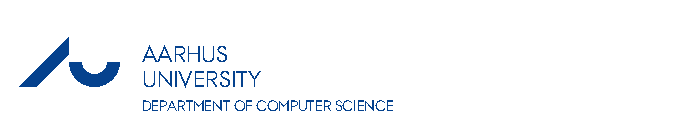
\epsfig{file=logo.eps}\clearpage

%%%%%%%%%%%%%%%%%%%%%%%%%%%%%%%%%%%%%%%%%%%%%%%%%%%%%%%%%%%%%%%%%%%%%%%

\pagestyle{plain}

%%%%%%%%%%%%%%%%%%%%%%%%%%%%%%%%%%%%%%%%%%%%%%%%%%%%%%%%%%%%%%%%%%%%%%%

\chapter*{Abstract}
\addcontentsline{toc}{chapter}{Abstract}

Ensuring correctness of programs is of ever-growing importance as software increasingly handles safety-critical functions. The surge of concurrent programs makes this task significantly more challenging. This thesis focuses on queue algorithms which are commonly used in a concurrent setting.\\
To reason formally about queues, we use the Iris program logic. After giving a brief introduction to the logic, we use it to express three queue specifications. The most general of these is the ``HOCAP-style'' specification, which supports concurrent clients and allows tracking of queue contents. We demonstrate that this specification implies the other, simpler specifications.\\
The project then examines two queue algorithms: the blocking and non-blocking Michael-Scott Queues. We give implementations for these algorithms in the programming language \heaplang{}. Both implementations are proven to satisfy the HOCAP-style specification. The blocking Michael-Scott Queue is verified using an invariant that tracks the contents of the queue and specifies the possible states of the queue data structure. For the non-blocking Michael-Scott Queue, a notion of reachability, borrowed from existing work, is incorporated into its invariant to meet the HOCAP-style specification. All proofs developed in this project have been mechanised in the Coq proof assistant.

%%%%%%%%%%%%%%%%%%%%%%%%%%%%%%%%%%%%%%%%%%%%%%%%%%%%%%%%%%%%%%%%%%%%%%%

\chapter*{Resum\'e}
\addcontentsline{toc}{chapter}{Resum\'e}

I forbindelse med at software overtager flere sikkerheds-kritiske opgaver stiger vigtigheden af verificering af software. Den øgede popularitet af ``parallelprogrammering'' gør denne verificerings-opgave markant mere udfordrende. Dette speciale fokuser på kø-algoritmer, som ofte bruges i parallelprogrammering.\\
Vi bruger program logikken Iris til at ræsonnere formelt omkring køer. Efter en kort introduktion til logikken anvender vi den til at udtrykke tre specifikationer for køer. Den mest generelle af disse er den såkaldte ``HOCAP-style'' specifikation, som tillader køen at blive brugt i parallelle sammenhænge, samt understøtte at klienter kan holde styr på køens indhold. Vi demonstrerer at køer, der overholder HOCAP-style specifikationen, også overholder de to andre specifikationer.\\
Projektet udforsker derefter to specifikke køer: den blokerende og ikke-blokerende Michael-Scott kø. Vi give implementeringer af køerne i programmeringssproget \heaplang{}. Det vises, at begge implementeringer overholder HOCAP-style specifikationen. Verifiseringen af den blokerende Michael-Scott kø fungerer ved brugen af en invariant, som holder styr på køens indhold, og specificerer de mulige tilstande, som køren kan være i. Invarianten for den ikke-blokerende Michael-Scott kø benytter ideen om ``reachability'' fra tidligere arbejde. Alle beviser fremstillet i projektet er blevet maskine-verificeret i bevis assistenten Coq.

%%%%%%%%%%%%%%%%%%%%%%%%%%%%%%%%%%%%%%%%%%%%%%%%%%%%%%%%%%%%%%%%%%%%%%%

\chapter*{Acknowledgments}
\addcontentsline{toc}{chapter}{Acknowledgments}

I would like to thank my advisor, Amin Timany, for giving great guidance and feedback and for being a great teacher in both this and previous projects.\\
A special thanks to my family who has given me support and encouragement throughout my studies.

\vspace{2ex}
\begin{flushright}
  \emph{Mathias Pedersen}\\
  \emph{Aarhus, \today.}
\end{flushright}

%%%%%%%%%%%%%%%%%%%%%%%%%%%%%%%%%%%%%%%%%%%%%%%%%%%%%%%%%%%%%%%%%%%%%%%

\tableofcontents
\cleardoublepage
\pagenumbering{arabic}
\setcounter{secnumdepth}{2}

%%%%%%%%%%%%%%%%%%%%%%%%%%%%%%%%%%%%%%%%%%%%%%%%%%%%%%%%%%%%%%%%%%%%%%%

\chapter{Introduction}
\label{ch:intro}

Correctness of software is of ever-growing importance as more and more safety-critical functions are entrusted to computers. As such, being able to verify the correctness of a piece of software has become highly desirable. With the surge of multiprocessor computing, the complexity of software systems has grown significantly. Reasoning about the correctness of concurrent programs is particularly tricky as one must reason about all possible interactions between participating threads.

A verification technique that gives very strong correctness guarantees is that of using a \textit{program logic}. The idea is to set up a formal system that captures the semantics of a programming language, which one can then use to derive (i.e. prove) formal descriptions of how specific expressions behave: a specification of the program. That is, the logic allows us to write formal program specifications and prove them. One such program logic is \textit{Iris}, a concurrent separation logic that supports reasoning about concurrent programs and how the resources these programs operate on are used by participating threads.

This project focuses on \textit{queues}. Using the aforementioned program logic, we give specifications for queue algorithms in general. These specifications vary in generality and complexity, reflecting the difficulties of reasoning about concurrent programs. The most general queue specification we develop is a so-called \textit{HOCAP-style} specification, which supports concurrent clients, and allows them to track the contents of the queue.

In this project, we study two concrete queue implementations, namely the blocking and non-blocking Michael-Scott Queues (\msq{}s for short). These queues demonstrate two of the most common synchronisation mechanisms: locks, which are blocking, and atomic instructions such as compare-and-swap, which are non-blocking.

Previous work \citep{DBLP:conf/cpp/VindumB21} has shown that the non-blocking \msq{} contextually refines a coarse-grained queue. However, this result does not allow clients of the queue to formally verify their own specifications using the logic.\\
As for the blocking \msq{}, no prior correctness results are known to this author. The original presentation of the queue \citep{DBLP:conf/podc/MichaelS96} gave an argument for its correctness, however, we demonstrate that the argument relies on an incorrect assumption.

This project makes the following contributions.
\begin{itemize}
  \item Giving three different specifications for queues at different levels of generality.
  \item Proving that both \msq{}s meet these specifications.
  \item Demonstrating that the HOCAP-style specification implies the other two specifications.
  \item Mechanising everything presented in this report in the Coq proof assistant.
\end{itemize}

The structure of the report is as follows. We begin in chapter \ref{ch:pre} with an exposition of the programming language used in the project, as well as the program logic, Iris. Following this, in chapter \ref{ch:QueueSpecs} we give the three queue specifications and discuss their capabilities. We further prove that the HOCAP-style specification can derive the other two specifications. Chapter \ref{ch:TLMSQ} discusses the \tlmsq{} and gives an implementation for it in our chosen programming language. We then proceed to prove that the implementation satisfies the three specifications in chapter \ref{ch:TLMSQSPECS}. In a similar way, chapter \ref{ch:LFMSQ} gives our implementation of the \lfmsq{}, and chapter \ref{ch:LFMSQSPECS} shows that it satisfies the HOCAP-style specification.

%%%%%%%%%%%%%%%%%%%%%%%%%%%%%%%%%%%%%%%%%%%%%%%%%%%%%%%%%%%%%%%%%%%%%%%

\chapter{Preliminaries}
\label{ch:pre}

This chapter covers some of the background topics that are required to understand the main parts of the project. Specifically, section \ref{Pre:section:heaplang} covers the basics of the language we use to implement the \msq{}s. Section \ref{Pre:section:iris} gives an overview of the program logic we use to reason about the queues. Finally, section \ref{Pre:section:coq} introduces the files containing the mechanisations of the work presented in this report.

%=====================================================================
\section{\heaplang}
\label{Pre:section:heaplang}

This project uses ``\heaplang'' as the implementation language. The main reason for this choice is that \heaplang is very well supported by the program logic Iris, which we introduce in the next section. However, \heaplang is still a quite suitable language for this project, as it has features to support faithful implementations of the \msq{}s. In particular, \heaplang is an untyped ML-style language and notably supports recursion, references, and concurrency. References are handled with a \textit{heap}, hence the name of the language. Only reference to values can be created. The instruction $\Ref(\val)$ allocates a spot on the heap containing $\val$ and returns the location, $\loc$, of the value. This location can then later be read using $\deref \loc$, or updated using $\loc \gets \val'$.

Concurrency is supported by the $\Fork{\expr}$ instruction. This instruction creates a new thread which executes $\expr$. Multiple threads can communicate through the heap, and to allow for synchronisation, \heaplang supports a compare-and-swap instruction. The instruction $\CAS \ \loc \ \val \ \val'$ atomically reads $\loc$, compares the contents with $\val$, and if similar, stores $\val'$ at $\loc$. If $\loc$ does not contain $\val$, no change occurs.

For the basic constructs, \heaplang supports basic arithmetic on integers, comparisons, conditionals, pairs and projections, and injections and pattern matching. Many of the other usual constructions expected of similar languages are achieve with syntactic sugar. For instance, we define the $\langkw{let}$ construction as $\Let \var = \expr_1 in \expr_2 \eqdef (\lambda{} \var . \expr_2) ~ \expr_1$. Similarly, we can support sequences of instructions by defining $\expr_1 ; \expr_2 \eqdef (\lambda{} \var . \expr_2) ~ \expr_1$, but where $\var$ is fresh.

The full specification of the language can be found in \citet{gentleiris} (section 2 at time of writing).

%=====================================================================
\section{The Iris Program Logic Framework}
\label{Pre:section:iris}

In this section, we give a brief introduction to Iris -- the logic we use to reason about the \msq{}s. Iris is quite expressive and supports a myriad of features and derived rules, many of which have been utilised in this project. As such, it will be impossible to cover all facets of Iris in detail, so we limit ourselves to give an overview of the main aspects of Iris. If the reader wishes a more thorough introduction, or wants to see further details of the topics covered, please consult the Iris Lecture Notes \citep{gentleiris}.

\subsection{Fundamentals of Iris}
Briefly put, Iris is a \enquote{Higher-Order Concurrent Separation Logic Framework}. The framework part means that Iris is not tied to a single programming language; one may instantiate Iris with any programming language one sees fit. The ``concurrent'' part implies that Iris supports reasoning about languages with concurrent features, such as \heaplang. In fact, \heaplang is a sort of ``default'' language which ships with Iris. As such, some of the rules we present in this section will be programming language independent, while others will adhere to the semantics of \heaplang.

A feature that makes Iris very powerful, is that it is a \textit{higher order logic}. This essentially means that we may quantify over propositions and predicates. This feature of Iris is essential to this project -- much of the work done relies on this capability.

As Iris is a separation logic, we can reason about ownership of \textit{resources}. Iris's notion of resources is very general due to \textit{resource algebras}, which we explain in section \ref{Pre:iris:sub:RA}, but a simple example is that of pointers. One may ``own'' a particular pointer which allows one to manipulate it. We capture this with the ``points-to'' predicate; the proposition $\loc \mapsto \val$ denotes ownership over location $\loc$, with the fact that $\loc$ points to $\val$. It guarantees that no other threads can interact with the location. Ownership of $\loc \mapsto \val$ can also be transferred to e.g. other threads, allowing them to interact with $\loc$. In general, propositions in Iris describe the resources that one owns.

Iris has usual connectives such as $\land$, $\lor$, and $\implies$, but with the addition of ownership, we additionally introduce \textit{separating conjunction}, written as: $P \star{} Q$, for propositions $P$ and $Q$. The proposition $P \star{} Q$ describes the resources in $P$ \emph{combined} with the resources in $Q$. Since ownership of a resource can be exclusive, it should not be freely duplicable. Hence, if we own some resources and wish to prove $Q_1 \star{} Q_2$, we must decide which resources we use to prove $Q_1$ and which resources to prove $Q_2$. This is captured by the \ruleref{star-I} rule. This is the main difference between regular conjunction and separating conjunction. We additionally introduce the ``wand'' connective, written $\wand$, which is similar to implication but works with separating conjunction instead. The introduction and elimination rules for wand (\ruleref{wand-I} and \ruleref{wand-E}) are hence similar to those for implication, but it takes the ownership aspect into consideration.
\begin{mathpar}
  \logicstarintrorule
  \and
  \logicwandintrorule
  \and
  \logicwandelimrule
\end{mathpar}

Ownership of resources does not have to be exclusive. For instance, if a location is never updated, then several threads should be allowed to have ownership over the points-to predicate for that location. To this end, Iris has the \textit{persistently modality}, written $\persistently P$ (read as ``persistently $P$''), which states that the resources described by $P$ are allowed to be duplicated (see rule \ruleref{persistently-dup}). Duplicability is an important capability; essential constructions in Iris rely on being duplicable as we explore in the next sections.\\
Propositions are persistent if they satisfy $P \proves \persistently P$. There are many rules which state how to derive and work with persistent propositions, but for the sake of brevity, we highlight here just two important rules: \ruleref{persistently-intro} and \ruleref{persistently-keep}. The first states that any proposition we prove from \emph{only} persistent proposition are themselves persistent, and the second states that we can use resources to prove persistent propositions without ``consuming'' the resources.
\begin{mathpar}
  \persduprule
  \and
  \persintrorule
  \and
  \perskeeprule
\end{mathpar}


\subsection{Hoare Triples and Weakest Pre-Condition}
The logic supports reasoning about programs via \textit{Hoare triples}. A Hoare triple $\hoare{P}{\expr}{\val . \Phi ~ \val}$ states that, if we own the resources described by $P$, then we may safely run $\expr$, and \emph{if} the computation terminates with value $\val$, then the predicate $\Phi$ holds of $\val$. That is, Hoare triples only show partial correctness of programs.

Specifications for functions are usually written in terms of Hoare-triples -- the pre-condition mentions which resources the function require and the post-condition states which resources the callee gets back, if the function returns. Hoare-triples are persistent (see rule \ruleref{persistently-Ht}), which allows clients to apply the same Hoare-triple for multiple invocations of the same function. This is sensible as the Hoare triple implies that the function only needs the resources described by the pre-condition in order to run safely; if we can get those resources multiple times, we can of course also run the function multiple times.

The rules for Hoare triples depend on the language. Figure \ref{Pre:iris:figure:hoare} shows some selected rules for the case of \heaplang{}. Some of the rules, such as \ruleref{Ht-alloc}, \ruleref{Ht-load-temp}, \ruleref{Ht-store-temp}, and \ruleref{Ht-beta} shows Hoare triples for basic constructs of the language. For example, \ruleref{Ht-alloc} states that it is always safe to create a new reference to some value, $u$, and the value returned from the creation is some location which points to $u$.

Other rules such as \ruleref{Ht-bind}, \ruleref{Ht-csq}, and \ruleref{Ht-frame} shows how to prove Hoare triples for more complex expressions. The bind rule allows us to ``focus'' on sub-expressions, as long as they are what will be executed next according to the semantics of the language. We must then prove a Hoare triple for the whole expression assuming that the sub-expression has reduced to some value. Note that the post-condition of the Hoare triple for the sub-expression becomes the pre-condition for Hoare triple of the whole expression.\\
The rule of consequence states that we can strengthen pre-conditions and weaken post-conditions. Indeed, if we can execute an expression with some resources, we can surely also execute it if we have \emph{more} resources available. Similarly, we can also simply decide to mention \emph{fewer} of the resources available after the function invocation.\\
The frame rule essentially states that resources which are not required to run the expression are not changed by it.

\begin{figure}
  \begin{mathpar}
    \pershtrule
    \and
    \htret
    \and
    \htbind
    \and
    \htalloc
    \and
    \htloadtemp
    \and
    \htstoretemp
    \and
    \htbeta
    \and
    \and
    \htcsq
    \and
    \htframe
  \end{mathpar}
  \caption{Selected rules for Hoare triples.}
  \label{Pre:iris:figure:hoare}
\end{figure}

Another way to reason about programs in Iris is \textit{weakest pre-condition}, written $\wpre{\expr}{\val .\Phi ~ \val}$. The main difference between weakest pre-conditions and Hoare triples is that the former does not mention the required resources in a pre-condition -- instead, propositions describing the required resources \emph{implies} the weakest pre-conditions. For instance, if one owns the points-to predicate for some location $\loc$, then one can derive a weakest pre-condition of a load of $\loc$. That is, we have that $\loc \pointsto \val \proves{} \wpre {\deref \loc}{u.u = v \ast \loc \pointsto \val}$.

The rules for weakest pre-conditions are analogous to the rules for Hoare triples shown in \ref{Pre:iris:figure:hoare}, so we do not mention them here. Indeed, we may even define the notions in terms of each other. The reason for having both is that it is usually nicer to write specifications in terms of Hoare triples, whereas proofs of weakest pre-conditions are more streamlined.

\subsection{Later Modality}
\label{Pre:iris:sub:later}

The presentation we have seen thus far does not allow us to tie propositions to steps in the program; we may want to express that some proposition holds after one program step. To achieve this, Iris provides a \textit{later} modality, written $\later P$. The later modality is technically language independent and hence parallel to program steps, but the way that Hoare triples and weakest pre-conditions are defined ties a single $\later$ to a single step in the program. For instance $\later (\loc \mapsto 5)$ asserts that the location $\loc$ will contain the value $5$ after taking one step in the program. In other words, we do not own the resource that $\loc$ points to $5$ now, but we will own it after one step. In this sense, the later modality weakens propositions; owning a resource now is stronger than owning it later (cf. rule \ruleref{Later-weak}).

We update the rules from figure \ref{Pre:iris:figure:hoare} to capture the effect that taking a step removes a later. For instance, \ruleref{Ht-beta-later-later} is similar to \ruleref{Ht-beta}, but it strips away a later in the pre-condition to signify that the program has taken a step (in this case by computing the function application).

The later modality has many uses in Iris, but for our presentation, the Löb induction rule, \ruleref{Loeb}, is the most important. It states that, if we want to prove some proposition $P$, we may assume that we have $P$ later. This rule is really useful when $P$ is a Hoare triple for a recursive function. If $f$ is some recursive function and we want to prove the Hoare triple: $\hoare{Q}{f ~ u}{v. \Phi ~ v}$, then Löb induction gives us an induction hypothesis: $\later (\hoare{Q}{f ~ u}{v. \Phi ~ v})$. As the later modality weakens our proposition, we cannot use it to prove our goal, but after performing the function application using \ruleref{Ht-beta}, the $\later$ in our induction hypothesis is stripped away, and we get to assume $\hoare{Q}{f ~ u}{v. \Phi ~ v}$. Hence, if we reach a recursive call inside $f$, we just have to prove $Q$, and then we can use our induction hypothesis to prove the recursive call.

\begin{mathpar}
  \laterweakrule
  \and
  \latermonorule
  \and
  \lobrule
  \and
  \htbetalater
  \and
  \and
  \htloadlaterrule
  \and
  \htstorelaterrule
\end{mathpar}

\subsection{Resource Algebra}
\label{Pre:iris:sub:RA}

Thus far, the only kind of resource we have seen are the points-to predicate. This is in itself a very useful notion of resource, but many constructions demand other kinds of resources. Iris allows us to create our own notion of a resource by defining a \textit{resource algebra} which specifies what the resources are, and how the resources interact with each other. Indeed, even the points-to predicate is defined via a resource algebra.

Formally, \blockquote[\citet{gentleiris}]{A \emph{resource algebra} is a commutative semigroup $\Ml$ together with a subset $\Vl \subseteq \Ml$ of elements called \emph{valid}, and a \emph{partial} function $\mcore{\cdot} : \Ml \to \Ml$, called the \emph{core}.}

That is, a resource algebra consists of a set of elements (the resources) with an associative and commutative operation, written as $a \mtimes b$. The set of elements is usually called the ``carrier''. Some of the elements are marked as ``valid'' -- only valid resources can be owned in Iris (cf. rule \ruleref{Own-valid}). Ownership of a non-valid element allows for deriving falsehood.\\
The core function ``extracts'' duplicable parts from resources. In particular, if the core of an element $a$ is $a$ itself, i.e. $\mcore{a} = a$, then $a$ is freely duplicable. Hence, ownership of $a$ is persistent.\\
Some resource algebra enjoy the additional property of being \textit{unital}. This essentially means that the carrier contains a unit element $\epsilon$ with respect to `$\mtimes$' which is both valid and duplicable.\\
Finally, we note that we can create a pre-order relation for every resource algebra by defining the extension order: $a \mincl b \iff \exists c, b = a \cdot c$.

Since programs update resources, we will need some way of updating elements in a resource algebra. We write $a \mupd b$ to mean that $a$ can be updated to $b$. Updates of elements should not be able to happen freely; a thread updating its resources should not invalidate the resources that another thread owns. The idea is to ensure that we can only update our resources if we do not make other resources invalid. We call such an update a \textit{frame preserving update}, and define as follows.
\begin{equation*}
  \fpurule
\end{equation*}
This rule is simplified a little, but it suffices of our purposes. It requires that any other resource that is valid with $a$ is also valid with $b$. This ensures us that we do not invalidate other elements as a consequence of the update.

\citet{gentleiris} shows many examples of basic resource algebra. However, it turns out that often, the desired construction can be realised by \emph{composing} different resource algebra, instead of defining them from the ground up. In fact, in this project, the resource algebras used were exclusively constructed from other resource algebra. Chapter \ref{ch:RA} shows the main resource algebras used in this project.\\
In this report, we isolate the difficulties of creating desired constructions by postulating their existence, and only later, in chapter \ref{ch:RA}, showing how to realise these using specific resource algebra.

\subsubsection{Ghost State}
We have until now only discussed resource algebra as an isolated concept. Now we show how resource algebras are tied into the logic of Iris, allowing us to use them in reasoning about programs.

The first component we need is an \textit{update modality}, written $\pvs P$. This modality governs where we are allowed to updated our resources, including the creation of new resources. We present the following three rules for introducing update modalities.
\begin{mathpar}
  \updmonorule
  \and
  \updintrorule
  \and
  \htcsqvsrule
\end{mathpar}
Here, the \textit{view-shift}, $\vs$, is defined as $P \vs Q = \persistently(P \implies \pvs Q)$, and states that, if we own the resources described by $P$, then we can derive the resources described by $Q$ after updating our resources (for instance via a frame preserving update).

Iris supports reasoning about resource algebra via the notion of \textit{ghost state}: for a resource algebra $\Ml$ and an element $a$ in the carrier, the assertion $\ownGhost{\gname}{a}$ denotes ownership over an instance of the resource $a$. Here $\gname$ is a \textit{ghost name} -- it gives a way to refer specific instances of the resource algebra. The following four rules demonstrate how to create, update, and reason about ghost resources in Iris.
\begin{mathpar}
  \ghostallocrule
  \and
  \ghostupdaterule
  \and
  \ownoprule
  \and
  \ownvalidrule
\end{mathpar}


\subsection{Invariants}
The last feature of Iris we need is that of \textit{invariants}. Some resources are required by multiple threads, but those resources may not be persistent, and hence not duplicable. To get around this, one can devise an invariant for said resources -- a proposition $P$, which describes the resources in a way that is always true. Then, one can assert that this proposition is an invariant, written $\knowInv{\Nl}{P}$, and since invariant are persistent, they can be given to multiple threads. The threads may then access the resources inside the invariant by \textit{opening} it. There are three criteria when opening an invariant. Firstly, the invariant can only be open for one program step. This is enforced by making the opening rule for invariants require that the expression in the Hoare triple or weakest pre-condition is ``atomic''. We can usually always satisfy this criteria by applying the \ruleref{Ht-bind} rule.\\
The second criteria is that the invariant can only be opened once, before being closed again. Iris enforces this by attaching masks to many of the constructs presented in the previous sections. The details of masks are not important for our presentation. Masks tell us which invariants we are allowed to open. For instance, the invariant opening rule for weakest pre-conditions, \ruleref{wp-inv-open-namespace}, attaches the mask $\mask\setminus\Nl^\uparrow$ to the weakest pre-condition, signifying that we cannot use invariants in the namespace $\Nl$ to prove the weakest pre-condition.\\
Finally, as \ruleref{wp-inv-open-namespace} also shows, we must prove that the invariant still holds after $\expr$ has taken its one step (this is realised by having $P$ in the post-condition). The reason is that other threads might also rely on the invariant, hence we have to reinstate it immediately.

\begin{mathpar}
  \invalloc
  \and
  \wpinvopen
\end{mathpar}

A technicality of invariants is that we only get the resources \emph{later} when opening them.\footnote{Getting the resources immediately would be unsound.} This is usually not an issue as most of the rules for stepping through programs only require resources later (cf. section \ref{Pre:iris:sub:later}). Hence we will usually assume that we have resources available \emph{now}, when we open invariants. We mention the later explicitly in the few cases where only getting the resources later is important.

\subsection{Locks}\label{Pre:iris:locks}

The \tlmsq{} uses locks, so we discuss these briefly in this section. A lock has three functions: $\newLock$, $\acquire$, and $\release$. In Iris, locks protect resources; when we create a new lock we give it the resources it must protect. When a thread acquires the lock, the thread gets access to the protected resources. Releasing the locks then requires that the resources are transferred back to the lock. In our project, we use the following specification for locks from \citet{gentleiris} (example 8.38 at time of writing).
\begin{align*}
  &\Exists \isLock : \Val \to \Prop \to \textlog{GhostName} \to \Prop.\nonumber\\
  &\Exists \locked : \textlog{GhostName} \to \Prop.\nonumber\\
  &\quad\quad\persistently(\All P, v, \gamma. \isLock(v,P,\gamma) \implies \persistently \isLock(v,P,\gamma))\\
  &\land\quad\persistently(\All \gamma. \locked(\gamma) \ast \locked(\gamma) \implies \FALSE)\\
  &\land\quad\All P.\hoare{P}{\newLock ()}{v.\Exists \gamma.\isLock(v,P,\gamma)}\\
  &\land\quad\All P, v, \gamma.\hoare{\isLock(v,P,\gamma)}{\acquire v}{\_.P \ast \locked(\gamma)}\\
  &\land\quad\All P, v, \gamma.\hoare{\isLock(v,P,\gamma) \ast P \ast \locked(\gamma)}{\release v}{\_.\TRUE}
\end{align*}
The specification assert the existence of two predicates: the lock predicate, ``$\isLock$'' and a lock token, ``$\locked$''. The lock predicate describes that a value represents a lock, and governs which resources the lock protects. The specification for the $\newLock$ function states that if we own the resources described by $P$, we can create a new lock by invoking $\newLock$. The value returned by the function then represents the lock, and it protects the resources described by $P$. The lock predicate is persistent so we can give the lock predicate to multiple threads, allowing them to use the specifications for $\acquire$ and $\release$. The specification for $\acquire$ grants us access to the resources that the lock is protecting as well as a non-duplicable token, $\locked(\gname)$. This token tells us that we are the sole owner of the lock. To release the lock, we must give up the $\locked(\gname)$ token and the resources the lock protects.

%=====================================================================
\section{Formalisation in Coq}
\label{Pre:section:coq}

Iris has been mechanised in the Coq proof assistant\footnote{The mechanisation can be found at \url{https://gitlab.mpi-sws.org/iris/iris/}} -- a tool to machine-check proofs of mathematical assertions. All results in this project have been completely machine-verified in the Iris mechanisation in Coq. Specifications in the Coq formalisation of Iris are usually written in terms of Hoare triples but proved by first converting the Hoare triples to equivalent weakest pre-conditions, as this is usually easier to work with. The proofs presented in this report will follow suit and give specifications using Hoare triples, but prove them assuming they are weakest pre-conditions. The proofs presented in the report thus follow the mechanised proofs very closely, making it possible to ``step-through'' the mechanised proofs in tandem with reading the paper-proofs presented in this report.

One caveat is that there is somewhat of a discrepancy between Iris on paper, and the Iris formalisation in Coq. Working with the latter requires a bit deeper understanding of the model of Iris. \citet{DBLP:journals/jfp/JungKJBBD18} explains the underlying model of an older version of Iris, but many of the concepts discussed are still relevant.\footnote{For an up-to-date presentation, consult the Technical Reference at \url{https://iris-project.org/}}

Table \ref{Pre:files-table} gives an overview of the files developed in the project and how they relate to this report. All files related to the project are available at \url{https://github.com/MatteP1/thesis}.

\begin{table}[h]
\begin{adjustbox}{center}
\begin{tabularx}{\textwidth}{llX}
  \toprule
  \textbf{File Name} & \textbf{Relevant Sections} & \textbf{Description} \\
  \midrule
  \path{queue_specs.v} & Chapter \ref{ch:QueueSpecs} & \multirow{2}{\linewidth}{Queue specifications and derivations, and an example client.} \\
  \path{queue_client.v} & Section \ref{QueueSpecs:section:queueadd} & \\
  \midrule
  \path{MSQ_common.v} & Chapters \ref{ch:TLMSQ} - \ref{ch:LFMSQSPECS} & Common definitions and lemmas. \\
  \midrule
  \path{twoLockMSQ_impl.v} & Chapter \ref{ch:TLMSQ} & \multirow{4}{\linewidth}{\tlmsq{} implementation and proofs of sequential, concurrent, and HOCAP-style specifications.} \\
  \path{twoLockMSQ_sequential_spec.v} & Section \ref{TLMSQSPECS:section:sequential} & \\
  \path{twoLockMSQ_concurrent_spec.v} & Section \ref{TLMSQSPECS:section:concurrent} & \\
  \path{twoLockMSQ_hocap_spec.v} & Section \ref{TLMSQSPECS:section:hocap}& \\
  \midrule
  \path{lockFreeMSQ_impl.v} & Chapter \ref{ch:LFMSQ} & \multirow{2}{\linewidth}{\lfmsq{} implementation and HOCAP-style specification proof.} \\
  \path{lockFreeMSQ_hocap_spec.v} & Chapter \ref{ch:LFMSQSPECS} & \\
  \midrule
  \path{lockAndCCFreeMSQ_impl.v} & Section \ref{LFMSQSPECS:section:discussion} & \multirow{2}{\linewidth}{Consistency-Check-Free version of \lfmsq{}.}\\
  \path{lockAndCCFreeMSQ_hocap_spec.v} & Section \ref{LFMSQSPECS:section:discussion}& \\
  \bottomrule
\end{tabularx}
\end{adjustbox}
\caption{Overview of Coq Files.}
\label{Pre:files-table}
\end{table}

\subsection{Compiling the Project}
Compiling the project requires both Coq and Iris to be installed. Once installed, open a terminal and navigate to the project folder, \path{/thesis}, which contains the \path{_CoqProject} file. Here, run \mintinline{shell-session}{make}. This will both create a Coq Makefile and run it. The project is known to compile with Coq version 8.19.0 and Iris version 4.2.0.

%%%%%%%%%%%%%%%%%%%%%%%%%%%%%%%%%%%%%%%%%%%%%%%%%%%%%%%%%%%%%%%%%%%%%%%

\chapter{Queue Specifications}
\label{ch:QueueSpecs}

%=====================================================================
\section{Specifications for Queues}
\label{QueueSpecs:section:specs}

In this chapter we discuss some possible specifications for queue data structures in general. As such, we need to make some basic assumption about what we expect from a queue. Firstly, we adopt the convention that a queue consists of three functions: $\initialise$, $\enqueue$, and $\dequeue$. Exactly what these functions do depends on the specific implementation of the queue, but we give some general pointers to what we expect of them.\\
The $\initialise$ function should create a queue which is initially empty. The functions $\enqueue$ and $\dequeue$ can then be invoked subsequently on said queue.\\
In addition to being parametrised on the queue, the $\enqueue$ function should also take a value as input. When invoking $\enqueue$ with such a value, the function should add this value to the end of the queue.\\
The $\dequeue$ function attempts to dequeue an element from the queue. Since queues are allowed to be empty, the $\dequeue$ function is assumed to return an option value. If the queue is empty, then $\dequeue$ should return $\None$, and otherwise it should remove an element from the front of the queue, and return this wrapped in a $\Some$.

Working in a concurrent setting often gets quite complicated quite fast, and proving that ones queue satisfies the above desirables can become quite tricky. In fact, even defining those qualities formally can become non-trivial. As such, we give three different specifications for queues. In section \ref{QueueSpecs:section:seq} we give a specification that assumes the queue is run in a sequential setting. Next, in section \ref{QueueSpecs:section:conc}, we give a specification that \textit{does} allow for concurrency but gives up on some of the above qualities. Primarily, it does not track the contents of the queue; invoking $\enqueue$ on a value does not guarantee that the value is added to the queue. Finally, in section \ref{QueueSpecs:section:hocap} we give a specification that allows for both concurrency \textit{and} tracking of the contents of the queue.

%=====================================================================
\section{Defining a Sequential Specification}
\label{QueueSpecs:section:seq}

Let us first consider a specification in the simple case where we do not allow for concurrency. In this case, we know that only a single thread will interact with the queue at any given point in a sequential manner. The specification we give will track the exact contents of the queue. To this end, we shall define the \textit{abstract state} of the queue, denoted $\absvalueList$ as a list of \heaplang values. That is, $\absvalueList : \List ~ \Val$. We adopt the convention that enqueueing an element is done by adding it to the front of the list, and dequeueing removes the last element of the list (if such an element exists). The reason for this choice is purely technical.

To allow queues to use whichever ghost names they like, we introduce the type ``$\SeqQgnames$'' whose purpose is to keep track of the ghost names used for a specific queue. One may think of $\SeqQgnames$ as set of fixed-length tuples of ghost names.

With this, we give our definition of a sequential specification for a queue.
\begin{definition}[Sequential Specification]\label{QueueSpecs:spec:seq}
\begin{align*}
  &\Exists \isqueueseq : \Val \to \List ~ \Val \to \SeqQgnames \to \Prop.\\
  &\quad\quad\seqspecinit\\
  &\land{}\quad\seqspecenq\\
  &\land{}\quad\seqspecdeq
\end{align*}
\end{definition}

The proposition $\isqueueseq(\vq, \absvalueList, \Qg)$ captures that the value $\vq$ is a queue, whose contents matches that of our abstract representation $\absvalueList$, and the queue uses the ghost names described by $\Qg$. Clients of a queue satisfying this specification can then apply the three Hoare triples at invocations for $\initialise$, $\enqueue$, and $\dequeue$, which tells them how the queue changes as a result of the invocation.\\
Note that the $\isqueueseq$ predicate is not required to be persistent, hence it cannot be duplicated and given to multiple threads. Since this predicate is required to apply the Hoare triples, then only a single thread can use the specification at a time. This is the sense in which the specification is sequential.

%=====================================================================
\section{Defining a Concurrent Specification}
\label{QueueSpecs:section:conc}

As discussed in the previous section, a concurrent specification will need the queue predicate to be duplicable to allow multiple threads to use the specification concurrently. For this specification, we denote the queue predicate by $\isqueueconc$.

To achieve duplicability of $\isqueueconc$, we shall give up on tracking the abstract state of the queue. The reason for doing so is the following. Consider the case where we own the queue predicate and it states that the abstract state of queue is $\absvalueList$. We spawn two threads and give them both the queue predicate stating that the abstract value is $\absvalueList$. Now they both invoke $\enqueue$, one with value $\absvalue$ and the other with $\absvalue'$. This makes one thread conclude that the abstract state of the queue is $\absvalue \catenate \absvalueList$, and the other that it is $\absvalue' \catenate \absvalueList$, whereas in reality, the queue contains both $\absvalue$ and $\absvalue'$. This is of course not desirable, and it is not immediately obvious how to solve this issue.

We \textit{can} however make the queue guarantee that a given property holds of all the values in the queue. We do this by parametrising $\isqueueconc$ with a predicate, $\Psi$, which it will maintain holds for all elements in the queue. In this way, when dequeueing, we at least know that if we get some value, then $\Psi$ holds of this value. The specification we wish to prove is as follows.
\begin{definition}[Concurrent Specification]\label{QueueSpecs:spec:conc}
\begin{align*}
  &\Exists \isqueueconc : (\Val \to \Prop) \to \Val \to \ConcQgnames \to \Prop.\\
  &\All \Psi : \Val \to \Prop.\\
  &\quad\quad \All \vq, \Qg . \isqueueconc(\Psi, \vq, \Qg) \implies \persistently \isqueueconc(\Psi, \vq, \Qg)\\
  &\land{}\quad\concspecinit{\Psi}\\
  &\land{}\quad\concspecenq{\Psi}\\
  &\land{}\quad\concspecdeq{\Psi}
\end{align*}
\end{definition}
This specification additionally requires that $\isqueueconc$ is persistent, which means that it can be duplicated and given to multiple threads. We again use a collection of ghost names, which we here denote $\ConcQgnames$.

%=====================================================================
\section{Defining a HOCAP-style Specification}
\label{QueueSpecs:section:hocap}

In this section we explore our most general specification: one that allows for both concurrency and tracking of the contents of the queue. We refer to this specification as a HOCAP-style specification -- Higher Order Concurrent Abstract Predicate -- since it is concurrent and parametrised by abstract predicates. This specification is more general than both the sequential and concurrent specifications in the sense that they are derivable from the HOCAP-style specification. We prove this in section \ref{QueueSpecs:section:deriving-seq-and-conc}.

As with the concurrent specification, we cannot simply parametrise the queue predicate (now denoted $\isqueue$) with the abstract state of the queue. So to allow clients to keep track of the contents of the queue, we ``split'' the abstract state into two parts; the authoritative view and the fragmental view. The clients will then own the fragmental view, allowing them to keep track of the contents of the queue, whereas the $\isqueue$ predicate will own the authoritative view. We will in particular make sure that, if one has both the fragmental and authoritative views, then these agree on the abstract state of the queue. Further, it is only possible to update the abstract state of the queue if one possess both the authoritative and fragmental views. Hence, clients will have to supply the fragmental view to be able to apply the specifications for $\enqueue$ and $\dequeue$.

For an abstract state $\absvalueList$ and a ghost name $\gname$, we shall use the notation $\abstractstateauth{\gname}{\absvalueList}$ to mean that the authoritative view of the abstract state associated with $\gname$ is $\absvalueList$. Similarly we write $\abstractstatefullfrag{\gname}{\absvalueList}$ to mean that the fragmental view associated with $\gname$ is $\absvalueList$.

We introduce three lemmas to help working with these predicates. These are proved in section \ref{RA:sections:abstract-state}. The first lemma shows that we can create fresh authoritative and fragmental views for any abstract state. Although, the abstract state is usually empty when allocating.
\begin{restatable}[Abstract State Alloc]{lemma}{abstalloc}\label{lemma:abst:alloc}
  For any abstract state $\absvalueList$, we have
  \begin{equation*}
    \proves \pvs \Exists \gname . \abstractstateauth{\gname}{\absvalueList} \star{} \abstractstatefullfrag{\gname}{\absvalueList}
  \end{equation*}
\end{restatable}

The second shows that the authoritative and fragmental views of the abstract state agree.
\begin{restatable}[Abstract State Agree]{lemma}{abstagree}\label{lemma:abst:agree}
  For a ghost name $\gname$ and abstract states $\absvalueList$ and $\absvalueList'$, we have
  \begin{equation*}
    \abstractstateauth{\gname}{\absvalueList'} \star{}
    \abstractstatefullfrag{\gname}{\absvalueList} \proves
    \absvalueList = \absvalueList'
  \end{equation*}
\end{restatable}

The final lemma shows that, if we own both the authoritative and fragmental views, we are allowed to update the abstract state to whatever we like.
\begin{restatable}[Abstract State Update]{lemma}{abstupdate}\label{lemma:abst:update}
  For any ghost name $\gname$, and abstract values $\absvalueList$, $\absvalueList'$, and $\absvalueList''$, we have
  \begin{equation*}
    \abstractstateauth{\gname}{\absvalueList'} \star{}
    \abstractstatefullfrag{\gname}{\absvalueList} \vs
    \abstractstateauth{\gname}{\absvalueList''} \star{}
    \abstractstatefullfrag{\gname}{\absvalueList''}
  \end{equation*}
\end{restatable}

The collection of ghost names is now denoted $\Qgnames$, but as all queues have to deal with the ghost name keeping track of the abstract state as describe above, we require that any $\Qgnames$ contains a ghost name used for this purpose. We shall refer to this ghost name as $\gabst$.

With this, we now give the HOCAP-style specification, and explain the intricacies of it afterwards.
\begin{definition}[HOCAP Specification]\label{QueueSpecs:spec:hocap}
\begin{align*}
  &\Exists \isqueue : \Val \to \Qgnames \to \Prop.\\
  &\quad\quad \All \vq, \Qg . \isqueue(\vq, \Qg) \implies \persistently \isqueue(\vq, \Qg)\\
  &\land{}\quad\hocapspecinit\\
  &\land{}\quad\hocapspecenq\\
  &\land{}\quad\hocapspecdeq
\end{align*}
\end{definition}
As for the concurrent specification, we require that the queue predicate, $\isqueue$, is persistent, giving us support for concurrent clients.

Next, the specification for $\initialise$ gives clients an additional resource in the post-condition: the ownership of the fragmental view of the empty list, $\abstractstatefullfrag{\Qg.\gabst}{[]}$. As discussed above, this allows them to keep track of the contents of the queue.

The specifications for $\enqueue$ and $\dequeue$ have now been parametrised by two predicates: $P$ and $Q$. The clients get to pick $P$ and $Q$, and the choice depends on what the client wishes to prove; $P$ describes those resources that the client has before $\enqueue$ or $\dequeue$, and $Q$ the resources it will have after. Hence $P$ is in the pre-condition and $Q$ in the post-condition of the associated Hoare triples. However, before the client gets access to the Hoare triple for $\enqueue$ or $\dequeue$ they must prove a view-shift. This view-shift states how the abstract state of the queue will change as a result of running $\enqueue$ or $\dequeue$, and further shows that $P$ can be updated to $Q$. Note that the consequent of the view-shift contains a $\later$. This signifies that the update in the abstract state is tied to a step in the code. The mask on the view-shift further disallows opening of invariants in the namespace $\Nl.i$. This is to allow queues that use invariants to apply the view-shifts while their invariants are open (their invariants must of course be within the namespace $\Nl.i$).

It might seem a bit strange that the client has to prove that the abstract state can be updated, but remember that the client owns the fragmental view, and that both this and the authoritative view, which is owned by the queue, is needed to update the abstract state. When proving the view-shift, clients are not updating the abstract state of the queue, they are merely showing that they can supply the fragmental view, allowing the abstract state to be updated. This then enables the queue to update the authoritative view of the abstract state (using the proved view-shift) in conjunction with updating the concrete view.

Exactly how client supply the fragmental view depends on what the client wants to achieve. We will see two options, when we derive the sequential and concurrent specifications from this HOCAP-style specification in the next section.

%=====================================================================
\section{Deriving Sequential and Concurrent Specifications}
\label{QueueSpecs:section:deriving-seq-and-conc}

It is technically possible to derive the sequential and concurrent specifications from the HOCAP-style specification without having proven the HOCAP-style specification for a specific queue. However, it might be beneficial for the reader to first see how we can prove each specification \textit{directly} for a specific queue, which we show in chapter \ref{ch:TLMSQSPECS}, and then return to this section.


In this section we show that we can derive the sequential and concurrent specifications from sections \ref{QueueSpecs:section:seq} and \ref{QueueSpecs:section:conc} from the HOCAP-style specification we saw in the previous chapter. These derivations are implementation independent, so we assume that we have some functions $\initialise$, $\enqueue$, and $\dequeue$ which satisfy the HOCAP-style specification of definition \ref{QueueSpecs:spec:hocap}, and we wish to prove that they also satisfy the sequential and concurrent specifications of definitions \ref{QueueSpecs:spec:seq} and \ref{QueueSpecs:spec:conc}. That is, we assume that we have a collection of ghost names, $\Qgnames$, a persistent queue predicate, $\isqueue$, and the three HOCAP-style specifications for $\initialise$, $\enqueue$, and $\dequeue$. Both derivations simply use $\Qgnames$ as the collection of ghost names. So we let $\SeqQgnames$ and $\ConcQgnames$ be $\Qgnames$ in the following.

\subsection{Deriving the Sequential Specification}
Recall the sequential specification specified in definition \ref{QueueSpecs:spec:seq}. It demands a queue predicate, $\isqueueseq$. We here choose to define it as follows.
\begin{definition}[$\isqueueseq$ Predicate (Derive)]\label{QueueSpecs:spec:seq:isqueueseq_derive}
\begin{align*}
  \isqueueseq(\vq, \absvalueList, \Qg) \eqdef
    &\isqueue(\vq, \Qg) \star{}\\
    &\abstractstatefullfrag{\Qg.\gabst}{\absvalueList}
\end{align*}
\end{definition}
We proceed to prove the sequential specifications for the three queue functions.

\subsubsection{Sequential Initialise Specification}
Recall the sequential specification for initialise:
\begin{equation*}
  \seqspecinit
\end{equation*}
Unfolding $\isqueueseq$, this Hoare triple follows directly from the HOCAP-style initialise specification (cf. lemma \ref{QueueSpecs:spec:hocap}).

\subsubsection{Sequential Enqueue Specification}
The specification for $\enqueue$ states:
\begin{equation*}
  \seqspecenq
\end{equation*}
So assume some $\vq$, $\absvalue$, $\absvalueList$, and $\Qg$. Unfolding $\isqueueseq$, our goal becomes:
\begin{equation*}
  \hoare{\isqueue(\vq, \Qg) \star{} \abstractstatefullfrag{\Qg.\gabst}{\absvalueList}}{\enqueue \ \vq \ \absvalue}{\valB . \isqueue(\vq, \Qg) \star{} \abstractstatefullfrag{\Qg.\gabst}{(\absvalue :: \absvalueList)}}
\end{equation*}
To prove the Hoare triple, we shall use the HOCAP-style specification for enqueue. This however requires us to pick $P$ and $Q$, and prove the resulting view-shift.
We choose
\begin{align*}
  &P \eqdef \abstractstatefullfrag{\Qg.\gabst}{\absvalueList}&
  &Q \eqdef \abstractstatefullfrag{\Qg.\gabst}{(\absvalue :: \absvalueList)}
\end{align*}
and assume some $\absvalueList'$. We must then prove the view-shift:
\begin{equation*}
  \hocapspecenqVS{\absvalue}{\Qg}{\abstractstatefullfrag{\Qg.\gabst}{\absvalueList}}{\abstractstatefullfrag{\Qg.\gabst}{(\absvalue :: \absvalueList)}}{\absvalueList'}
\end{equation*}
Assume $\abstractstateauth{\Qg.\gabst}{\absvalueList'}$ and $\abstractstatefullfrag{\Qg.\gabst}{\absvalueList}$. By lemma \ref{lemma:abst:agree}, $\absvalueList = \absvalueList'$, hence, we can apply lemma \ref{lemma:abst:update} to update the authoritative and fragmental views to $(\absvalue :: \absvalueList)$, which exactly proves the consequent of the view-shift.\footnote{The consequent technically has a $\later$, but proving something \emph{now} is stronger than proving it \emph{later}.}

With this, we now get access to the following Hoare triple:
\begin{equation}
  \hocapspecenqHT{\vq}{\absvalue}{\Qg}{\abstractstatefullfrag{\Qg.\gabst}{\absvalueList}}{\abstractstatefullfrag{\Qg.\gabst}{(\absvalue :: \absvalueList)}}\label{QueueSpecs:spec:der:seq:proof:enq:hocap}
\end{equation}
The pre-condition already matches our goal, so we just have to get the post-condition to match. To do this, we must get $\isqueue(\vq, \Qg)$ in the post-condition of \ref{QueueSpecs:spec:der:seq:proof:enq:hocap}, but since $\isqueue(\vq, \Qg)$ is persistent and we have it in the pre-condition, we may also assume it in post-condition.

\subsubsection{Sequential Dequeue Specification}
We use a similar approach to above to prove the sequential dequeue specification:
\begin{equation*}
  \seqspecdeq
\end{equation*}
So we assume some $\vq$, $\absvalueList$, $\Qg$. We now instantiate the HOCAP-style dequeue specification with the following choices:
\begin{align*}
  P &\eqdef \abstractstatefullfrag{\Qg.\gabst}{\absvalueList}\\
  Q(\nodeval) &\eqdef \begin{array}{l}(\absvalueList = [] \star{} \nodeval = \None \star{} \abstractstatefullfrag{\Qg.\gabst}{\absvalueList}) \lor{}\\ (\Exists \absvalue, \absvalueList'. \absvalueList = \absvalueList' \catenate [\absvalue] \star{} \nodeval = \Some{\absvalue} \star{} \abstractstatefullfrag{\Qg.\gabst}{\absvalueList'})\end{array}
\end{align*}
We must now prove the resulting view-shift to get the Hoare triple (note that we have not substituted in $Q$ for the sake of readability). So assume some $\absvalueList'$. We must show:
\begin{equation*}
\hocapspecdeqVS{\Qg}{\abstractstatefullfrag{\Qg.\gabst}{\absvalueList}}{Q}{\absvalueList'}
\end{equation*}
By lemma \ref{lemma:abst:agree}, $\absvalueList'$ must be equal to $\absvalueList$. We do a case analysis on $\absvalueList$. If $\absvalueList$ is empty, we prove the left disjunct in the consequent of the view-shift, \emph{without} updating the authoritative and fragmental views. If $\absvalueList$ is non-empty, i.e. $\absvalueList = \absvalueList'' \catenate [\absvalue]$ for some $\absvalueList''$ and $\absvalue$, then we prove the right-side of the consequent in the view-shift by using lemma \ref{lemma:abst:update} to update the authoritative and fragmental views to the new abstract state, $\absvalueList''$.

With this, we get access to the Hoare triple (now with $Q$ substituted in):
\begin{equation}
  \hoareV[t]{\isqueue(\vq, \Qg) \star{} \abstractstatefullfrag{\Qg.\gabst}{\absvalueList}}{\dequeue \ \vq}{\nodeval . \begin{array}{l}(\absvalueList = [] \star{} \nodeval = \None \star{} \abstractstatefullfrag{\Qg.\gabst}{\absvalueList}) \lor{}\\ (\Exists \absvalue, \absvalueList'. \absvalueList = \absvalueList' \catenate [\absvalue] \star{} \nodeval = \Some{\absvalue} \star{} \abstractstatefullfrag{\Qg.\gabst}{\absvalueList'})\end{array}}\label{QueueSpecs:spec:der:seq:proof:deq:hocap}
\end{equation}
As before, the only difference between this Hoare triple and the one we must prove is that we are missing $\isqueue(\vq, \Qg)$ in the post-condition. We can again get this from the fact that the queue predicate is persistent.

\subsection{Deriving the Concurrent Specification}
We prove the concurrent specification of definition \ref{QueueSpecs:spec:conc}. Remember that we need the $\isqueueconc$ predicate to be persistent, hence we cannot simply assert $\abstractstatefullfrag{\Qg.\gabst}{\absvalueList}$ as we did for $\isqueueseq$.\footnote{As we explain in section \ref{RA:sections:abstract-state}, no elements of the abstract state resource algebra are persistent.} Instead, we put it into an invariant. The queue predicate we use thus looks as follows.
\begin{definition}[$\isqueueconc$ Predicate (Derive)]\label{QueueSpecs:spec:conc:isqueueconc_derive}
\begin{align*}
  \isqueueconc(\Psi, \vq, \Qg) \eqdef
  &\isqueue(\vq, \Qg) \star{}\\
  &\knowInv{\Nl.c}{\Exists \absvalueList. \abstractstatefullfrag{\Qg.\gabst}{\absvalueList} \star{} \AllP(\absvalueList, \Psi)}
\end{align*}
\end{definition}
Persistency of $\isqueueconc$ follows by the persistency of $\isqueue$ and the fact that invariants are persistent.

\subsubsection{Concurrent Initialise Specification}
We have to derive the specification:
\begin{equation*}
  \concspecinit{\Psi}
\end{equation*}
As before, this specification only differs from the HOCAP-style specification for initialise in the post-condition. We use the \emph{generalised} rule of consequence \ruleref{Ht-csq-vs} and show that the post-condition of the HOCAP-style specification, i.e. $\Exists \Qg . \isqueue(\vq, \Qg) \star{} \abstractstatefullfrag{\Qg.\gabst}{[]}$, implies the post-condition above but with an update modality, $\pvs$, in front. Both mention the queue predicates, $\isqueue(\vq, \Qg)$, so it suffices to prove the invariant:
\begin{equation*}
  \pvs \knowInv{\Nl.c}{\Exists \absvalueList. \abstractstatefullfrag{\Qg.\gabst}{\absvalueList} \star{} \AllP(\absvalueList, \Psi)}
\end{equation*}
We have $\abstractstatefullfrag{\Qg.\gabst}{[]}$ from the HOCAP-style post-condition, and $\AllP([], \Psi)$ is equivalent to $\TRUE$. Hence, we can deduce $\Exists \absvalueList. \abstractstatefullfrag{\Qg.\gabst}{\absvalueList} \star{} \AllP(\absvalueList, \Psi)$. The rule \ruleref{Inv-alloc} shows us that we can turn this into the above invariant, so we are done.


\subsubsection{Concurrent Enqueue Specification}
We must derive:
\begin{equation*}
  \concspecenqGen{\Psi}{\vq}{\absvalue}{\Qg}
\end{equation*}
Assume some $\vq$, $\absvalue$, $\Qg$, and the invariant $\knowInv{\Nl.c}{\Exists \absvalueList. \abstractstatefullfrag{\Qg.\gabst}{\absvalueList}}$. Our goal becomes the following Hoare triple:
\begin{equation*}
  \hoare{\isqueue(\vq, \Qg) \star{} \Psi(\absvalue)}{\enqueue \ \vq \ \absvalue}{\valB . \TRUE}
\end{equation*}

We specialise the HOCAP-style enqueue specification with $P \eqdef \Psi(\absvalue)$ and $Q \eqdef \TRUE$. With this choice, the Hoare triple we get after proving the view-shift exactly matches our goal. Hence, we are done if we can prove the view-shift.

We assume $\absvalueList'$, and prove the view-shift:
\begin{equation*}
  \hocapspecenqVS{\absvalue}{\Qg}{\Psi(\absvalue)}{\TRUE}{\absvalueList'}
\end{equation*}
So assume $\abstractstateauth{\Qg.\gabst}{\absvalueList'}$ and $\Psi(\absvalue)$. We open the invariant giving us $\abstractstatefullfrag{\Qg.\gabst}{\absvalueList}$ and $\AllP(\absvalueList, \Psi)$ for some $\absvalueList$. By lemma \ref{lemma:abst:agree} we know that $\absvalueList = \absvalueList'$. We now update the abstract state to $(\absvalue :: \absvalueList)$ using lemma \ref{lemma:abst:update}, obtaining $\abstractstateauth{\Qg.\gabst}{(\absvalue :: \absvalueList)}$ and $\abstractstatefullfrag{\Qg.\gabst}{(\absvalue :: \absvalueList)}$. We use the first to prove the consequent of the view-shift. Before we are done, we must close the invariant. We use the fragmental part together with $\AllP(\absvalueList, \Psi)$ and $\Psi(\absvalue)$ to do this.

\subsubsection{Concurrent Dequeue Specification}
Finally, we derive the concurrent specification for $\dequeue$.
\begin{equation*}
  \concspecdeqGen{\Psi}{\vq}{\Qg}
\end{equation*}
So we assume some $\vq$, $\Qg$, $\Qg$, and the invariant. Our goal is now:
\begin{equation*}
  \hoare{\isqueue(\vq, \Qg)}{\dequeue \ \vq}{\nodeval . \nodeval = \None \lor{} (\Exists \absvalue. \nodeval = \Some \absvalue \star{} \Psi(\absvalue))}
\end{equation*}
We make the following choices for $P$ and $Q$ when instantiating the specification for $\dequeue$:
\begin{align*}
  &P \eqdef \TRUE&
  &Q(\nodeval) \eqdef \nodeval = \None \lor{} (\Exists \absvalue . \nodeval = \Some \absvalue \star{} \Psi(\absvalue))
\end{align*}
Again, with this choice, the Hoare triple we get after proving the view-shift exactly matches our goal.

We assume some $\absvalueList'$, and prove the view-shift (again, without substituting in $Q$):
\begin{equation*}
  \hocapspecdeqVS{\Qg}{\TRUE}{Q}{\absvalueList'}
\end{equation*}
Assume $\abstractstateauth{\Qg.\gabst}{\absvalueList'}$. Opening the invariant, we get $\AllP(\absvalueList, \Psi)$ and the fragmental part, $\abstractstatefullfrag{\Qg.\gabst}{\absvalueList}$, for some $\absvalueList$, which by lemma \ref{lemma:abst:agree} we know is equal to $\absvalueList'$. We proceed by case analysis on $\absvalueList$. If it is empty, we simply close the invariant again, and proceed to prove the first disjunct of the consequent. If it is not empty, then we have $\absvalueList = \absvalueList'' \catenate [\absvalue]$ for some $\absvalueList''$ and $\absvalue$. We use lemma \ref{lemma:abst:update} to update the abstract state to $\absvalueList''$, and split $\AllP(\absvalueList, \Psi)$ into $\Psi(\absvalue)$ and $\AllP(\absvalueList'', \Psi)$. Using this and the fragmental part, we close the invariant again. To finish, we prove the right disjunct of the consequent using the authoritative part and $\Psi(\absvalue)$.\footnote{Note here the importance of the $\later$ in the consequent. From the invariant, we technically only have $\later\Psi(\absvalue)$. If we did not have the later in the consequent, we would have to prove $\Psi(\absvalue)$ from $\later\Psi(\absvalue)$ which is not possible.}

%=====================================================================
\section{QueueAdd: An Example Queue Client}
\label{QueueSpecs:section:queueadd}
In this section, we look at an example queue client, named ``QueueAdd''. The example is somewhat contrived but illustrates the capabilities of the HOCAP-style specification and the limitations of the concurrent and sequential specifications.

The program is quite simple: it takes two integers $a$ and $b$ as input, and creates two threads that run in parallel. One thread enqueues $a$ and dequeues some element which is returned. The other thread does the same, except it enqueues $b$. The result of $\queueAdd$ is then the sum of the values dequeued by the threads: $a + b$. Figure \ref{QueueSpecs:queueadd:code} shows the program. Here, $e_1 \parcomp e_2$ is a construct for \textit{parallel composition}. It is syntactic sugar for an expression that runs $e_1$ and $e_2$ concurrently, waits for both computations to finish, and returns the results in a pair.

\begin{figure}
\begin{minted}[linenos=true, escapeinside=||, mathescape=true, bgcolor=codebg, frame=lines]{ocaml}
|$\label{UNW:def}$|  |$ \unwrap \ w \eqdef \langkw{match}\spac w \spac\langkw{with}\spac \None \Ra \TT \ \TT \mid \Some v \Ra v \spac\langkw{end} $|

|$\label{EDQ:def}$|  |$ \enqdeq \ \vq \ c \eqdef \enqueue \ \vq \ c; \unwrap (\dequeue \ \vq)$|

|$\label{QAD:def}$|  |$ \queueAdd \ a \ b \eqdef $|
|$\label{QAD:que}$|    |$ \Let \vq = \initialise \ \TT in $|
|$\label{QAD:spw}$|    |$ \Let p = (\enqdeq \ \vq \ a) \parcomp (\enqdeq \ \vq \ b) in $|
|$\label{QAD:add}$|    |$ \Fst p + \Snd p $|
\end{minted}
\caption{Implementation of $\queueAdd$.}
\label{QueueSpecs:queueadd:code}
\end{figure}

The specification for $\queueAdd$ essentially says that the return value is the sum of the inputs.
\begin{definition}[QueueAdd Specification]\label{QueueSpecs:spec:queueadd}
  \begin{equation*}
    \All a, b \in \mathbb{Z} . \hoare{\TRUE}{\queueAdd \ a \ b}{v . v = a + b}
  \end{equation*}
\end{definition}
\noindent This also implies that the program does not crash; the first case in the $\unwrap$ function never occurs.

Note first that, if we had not used parallel composition, and simply executed $\enqdeq$ twice in sequence, then the sequential specification would have sufficed in proving the specification. We would always have the $\isqueueseq$ predicate at hand to step through the $\enqueue$ and $\dequeue$ in the $\enqdeq$ function, and this would allow us to track the exact contents, which means that we could deduce that we never invoke $\dequeue$ when the queue is empty, and the dequeued values are exactly $a$ and $b$.\\
However, since $\isqueueseq$ is not persistent, it is not strong enough for the version using parallel composition. The specification for parallel composition, \ruleref{Ht-par}, states that we must decide which resources we give to each thread. We can not give both threads $\isqueueseq$ as it is not duplicable, but both threads will need the predicate in order to apply the specifications for $\enqueue$ and $\dequeue$.
\begin{mathpar}
  \Htpar
\end{mathpar}

The concurrent specification does not have this issue, as its queue predicate, $\isqueueconc$, \textit{is} persistent. However, the concurrent specification is not strong enough as it does not track the state of the queue. It is paramount for correctness that the $\dequeue$ in $\enqdeq$ does not result in $\None$; the $\unwrap$ crashes if it does. However, the concurrent specification only tells us that the $\dequeue$ is either $\None$ or $\Some \val$, for some value $\val$. We have no way of proving that it must be the latter case, as we do not track the contents of the queue.

We thus use the HOCAP-style specification, which allows us to track the contents of the queue, enabling us to exclude the cases where the dequeues result in $\None$. Further, we can argue about the actual values that are dequeued; it must be either a or b. The way we realise this, is by creating an invariant that captures the \textit{five} possible states of the queue, expressed by the fragmental view of the abstract state. The invariant looks as follows.\footnote{The variable $\QAg$ is a collection of ghost names used in proving the $\queueAdd$ specification. It contains four ghost names used for the four tokens.}
\begin{definition}[Invariant for QueueAdd]\label{QueueSpecs:queueadd:invariant}
  \begin{align*}
    \QueueAddInvariant(\Qg, \QAg, a, b) \eqdef~
    &\abstractstatefullfrag{\Qg.\gabst}{[]}~\star~\TokDoQAg~\star~\TokDtQAg~\lor\\
    &\abstractstatefullfrag{\Qg.\gabst}{[a]}~\star~\TokAQAg~\star~(\TokDoQAg~\lor~\TokDtQAg)~\lor\\
    &\abstractstatefullfrag{\Qg.\gabst}{[b]}~\star~\TokBQAg~\star~(\TokDoQAg~\lor~\TokDtQAg)~\lor\\
    &\abstractstatefullfrag{\Qg.\gabst}{[a; b]}~\star~\TokAQAg~\star~\TokBQAg~\lor\\
    &\abstractstatefullfrag{\Qg.\gabst}{[b; a]}~\star~\TokBQAg~\star~\TokAQAg~\lor
  \end{align*}
\end{definition}
Since invariants are persistent, we can give both the invariant and the HOCAP-style queue predicate to both threads, which gives the threads sufficient resources to use the HOCAP-style specifications for $\enqueue$ and $\dequeue$ when stepping through $\enqdeq$. The invariant also mentions four \textit{tokens}, $\TokDoQAg$, $\TokDtQAg$, $\TokAQAg$, and $\TokBQAg$. We discuss tokens further in section \ref{TLMSQSPECS:concurrent:sub:conc-queue-pred} and give the formal definition in section \ref{RA:sections:tokens}, but for this section it suffices to know that new tokens can always be created, and ownership of a token is \textit{exclusive}.\\
The idea is then that after applying the $\initialise$ specification on line \ref{QAD:que}, we create the four tokens and allocate invariant $\QueueAddInvariant$ in the first state, giving up $\TokDoQAg$ and $\TokDtQAg$, but keeping $\TokAQAg$ and $\TokBQAg$. When applying \ruleref{Ht-par}, we then give $\TokAQAg$ to the thread enqueueing $a$ and $\TokBQAg$ to the thread enqueueing $b$. When the threads prove the view-shift of the enqueue specification, they open the invariant in a state that does not mention their token. They then use lemma \ref{lemma:abst:update} to update the fragmental view so as to include the value they are enqueueing. When closing the invariant they give up the token associated with their value in exchange for a dequeue token: either $\TokDoQAg$ or $\TokDtQAg$. Thus, when they open the invariant to prove the view-shift of the $\dequeue$ specification, they will know that the queue is not empty, as that state mentions both dequeue tokens. Hence, they can perform the $\dequeue$, resulting in either $\Some a$ or $\Some b$, and obtain the associated token ($\TokAQAg$ or $\TokBQAg$). The unwrap hence does not crash, and we can use their tokens to conclude that one thread must have dequeued $a$ and the other $b$, hence proving the post-condition of the $\queueAdd$ specification.\\
We omit further details of the proof, and refer the interested reader to the formal proof in \path{queue_client.v}.

%%%%%%%%%%%%%%%%%%%%%%%%%%%%%%%%%%%%%%%%%%%%%%%%%%%%%%%%%%%%%%%%%%%%%%%

\chapter{The Two-Lock Michael-Scott Queue}
\label{ch:TLMSQ}

In this chapter, we give an implementation of the blocking version of the \msq{}, the \tlmsq{}, in \heaplang. This implementation differs slightly from the original, presented in \citet{DBLP:conf/podc/MichaelS96}, but most changes simply reflect the differences in the two languages.

%=====================================================================
\section{Introduction}
\label{TLMSQ:section:introduction}

This queue uses two locks to allow for enqueues and dequeues to happen concurrently; one lock protects the enqueue function, and another lock protects the dequeue function. The idea is to exploit the fact that removing elements through dequeue and adding elements through enqueue are largely orthogonal operations that do not clash with each other. Further, dequeues happen in one end of the queue and enqueues in the other, so they often operate on separate resources. When the queue is empty and they operate on the same resources, it becomes less trivial as to why this approach is safe. We shall explore this case in detail later.

The underlying data structure making up the queue is a singly-linked list. The linked-list always contains at least one element, called the \emph{head} node, marking the beginning of the queue. Note that the head node is itself not part of the queue, but all nodes following it are. The queue keeps a head pointer ($\lochead$) which always points to the head node, and a tail pointer ($\loctail$) which points to some node in the linked list, denoted the tail node.

In my implementation, a node is a triple $(\locinM{i}, \nodevalM{i}, \locoutM{i})$ satisfying that location $\locinM{i}$ points to the pair $(\nodevalM{i}, \locoutM{i})$. Here, $\nodevalM{i}$ either contains the value of the node $\absvalue_i$ wrapped in a $\Some$ (i.e. $\nodevalM{i} = \Some \absvalue_i$) or it is $\None$. The location $\locoutM{i}$ either points to $\None$ which represents the null pointer, or to the next node in the linked list. When we say that a location $\loc$ points to a node $(\locinM{i}, \nodevalM{i}, \locoutM{i})$, we mean that $\loc \mapsto \locinM{i}$. Hence, if we have two adjacent nodes $(\locinM{i}, \nodevalM{i}, \locoutM{i})$, $(\locinM{i+1}, \nodevalM{i+1}, \locoutM{i+1})$ in the linked list, then we have the following structure: $\locinM{i} \mapsto (\nodevalM{i}, \locoutM{i})$, $\locoutM{i} \mapsto \locinM{i+1}$, and $\locinM{i+1} \mapsto \nodevalM{i+1}, \locoutM{i+1}$.
For a given triple $\node = (\locin, \nodeval, \locout)$, we introduce the following notation:
\begin{align*}
  &\nIn{\node} = \locin& &\nVal{\node} = \nodeval& &\nOut{\node} = \locout
\end{align*}
This way of defining nodes essentially means that the ``in'' pointer becomes a sort of \textit{identifier} for the node. That is, if we have two nodes $\node$, $\node'$, and they agree on the ``in'' pointer, $\nIn{\node} = \nIn{\node'}$, then they are in fact the same node, $\node = \node'$. We capture this property formally in lemma \ref{lemma:nIn-equal}, which can be found in the appendix.

The reader may wonder why there is an extra, intermediary ``in'' pointer, between the pairs of the linked list, and why the ``out'' pointer could not point directly to the next pair. This comes down to difference between \heaplang and the C-like language used in the original implementation \citep{DBLP:conf/podc/MichaelS96}. Variables in the C-like language are technically just locations, and the assignment operator for variables simply corresponds to a store operation. In \heaplang, variables are modelled directly as locations which gives us an apparent extra pointer indirection compared to the original implementation.

%=====================================================================
\section{Implementation}
\label{TLMSQ:section:implementation}

The queue consists of 3 functions: $\initialise$, $\enqueue$, and $\dequeue$. Their implementation is shown in figure \ref{TLMSQ:impl:code}. As the name of the data structure suggests, the functions rely on two locks. To this end, we assume that we have some lock implementation given. In the accompanying Coq mechanisation, a ``spin-lock'' is used, but the only part we really care about is its specification which we discussed in section \ref{Pre:iris:locks}.

\subsection{Initialise}
\label{TLMSQ:implementation:sub:initialise}

The $\initialise$ function first creates a single node -- the head node -- marking the start of the linked list. It then creates two locks: the head lock, denoted $\Hlock$, protecting the head pointer, and the tail lock, denoted $\Tlock$, protecting the tail pointer. Finally, it creates the head and tail pointers, both pointing to the head node. The queue is then a pointer to a structure containing the head and tail pointers, and the two locks.

Figure \ref{TLMSQ:impl:figure:init} illustrates the structure of the queue after initialisation. Note that one of the pointers is decorated with a square. This represents a \emph{persistent} pointer; a pointer that will never be updated again. All ``in'' pointers $\locinM{i}$, are persistent, meaning that, once created, they will only ever point to $(\nodevalM{i}, \locoutM{i})$. We use the notation $\loc \mapsto^{\persistently} \val$ (introduced in \citet{DBLP:conf/cpp/VindumB21}) to mean that $\loc$ points to $\val$ persistently.

Note that in the original specification, a queue is a pointer to a 4-tuple $(\lochead, \loctail, \Hlock, \Tlock)$. Since \heaplang does not support 4-tuples, we instead represent the queue as a pointer to a pair of pairs: $\left((\lochead, \loctail), (\Hlock, \Tlock)\right)$.

\begin{figure}
  \centering
  \begin{adjustbox}{center}
  \begin{tikzpicture}[
    pair/.style = {
      on chain,
      rectangle split,
      rectangle split horizontal,
      rectangle split parts=2,
      draw,
      anchor=center,
      text height=1.5ex,
    },
    perspointer/.style = {
      on chain,
      rectangle,
      draw,
      anchor=center,
      text height=1.5ex,
    },
    pointer/.style = {
      rectangle,
      draw,
      anchor=center,
      text height=1.5ex,
    },
    start chain=going right,
    decoration={
      markings,
      mark=at position .5 with {\arrow{Square[length=5pt,sep=-2.5pt]}}
    },
  ]

  % Linked List
  \node (l'1) [join={by ->}, perspointer,on chain] {$\locinM{1}$};
  \node (l1pair) [join={by ->, draw=blue, postaction={decorate}}, pair,on chain] {$\None$ \nodepart{two} $\locoutM{1}$};
  \node (null) [join={by ->, draw=black}, rectangle,on chain] {$\None$};

  % Head and tail
  \node (head) [pointer, above left=of l'1] {$\lochead$};
  \node (tail) [pointer, above right=of l'1] {$\loctail$};
  \draw[->] (head) -- (l'1);
  \draw[->] (tail) -- (l'1);

  \end{tikzpicture}
  \end{adjustbox}
  \caption{Queue after initialisation.}
  \label{TLMSQ:impl:figure:init}
\end{figure}

\subsection{Enqueue}
\label{TLMSQ:implementation:sub:enqueue}

To enqueue a value, we create a new node, append it to the underlying linked-list, and swing the tail pointer to this new node. These three operations are depicted in figure \ref{TLMSQ:impl:figure:enqueue}.

The $\enqueue$ function takes as argument the value to be enqueued and creates a new node containing this value (corresponding to figure \ref{TLMSQ:impl:figure:enqueue:a}). This creation does not interact with the underlying queue data-structure, hence why we do not acquire $\Tlock$ first. After creating the new node, we must make the last node in the linked list point to it. Since this operation interacts with the queue, we first acquire $\Tlock$. Once we obtain the lock, we make the last node in the linked list point to our new node (figure \ref{TLMSQ:impl:figure:enqueue:b}). Following this, we swing $\loctail$ to the newly inserted node (figure \ref{TLMSQ:impl:figure:enqueue:c}).

Figure \ref{TLMSQ:impl:figure:enqueue} also illustrates when pointers become persistent; once the previous last node is updated to point to the newly inserted node, that pointer will never be updated again, hence becoming persistent.

\begin{figure}
  \centering
  \begin{subfigure}{\textwidth}
    \begin{adjustbox}{center}
    \begin{tikzpicture}[
      pair/.style = {
        on chain,
        rectangle split,
        rectangle split horizontal,
        rectangle split parts=2,
        draw,
        anchor=center,
        text height=1.5ex,
      },
      perspointer/.style = {
        on chain,
        rectangle,
        draw,
        anchor=center,
        text height=1.5ex,
      },
      pointer/.style = {
        rectangle,
        draw,
        anchor=center,
        text height=1.5ex,
      },
      start chain=going right,
      decoration={
        markings,
        mark=at position .5 with {\arrow{Square[length=5pt,sep=-2.5pt]}}
      },
    ]

    % Linked List
    \node (l'1) [join={by ->}, perspointer,on chain] {$\locinM{1}$};
    \node (l1pair) [join={by ->, draw=blue, postaction={decorate}}, pair,on chain] {$\nodevalM{1}$ \nodepart{two} $\locoutM{1}$};
    \node (l'2) [join={by ->, draw=blue, postaction={decorate}}, perspointer,on chain] {$\locinM{2}$};
    \node (l2pair) [join={by ->, draw=blue, postaction={decorate}}, pair,on chain] {$\nodevalM{2}$ \nodepart{two} $\locoutM{2}$};
    \node (null) [join={by ->, draw=black}, rectangle,on chain] {$\None$};

    \node (l'3) [perspointer, above right=of l2pair] {$\locinM{3}$};
    \node (l3pair) [join={by ->, draw=blue, postaction={decorate}}, pair,on chain] {$\nodevalM{3}$ \nodepart{two} $\locoutM{3}$};
    \node (null) [join={by ->, draw=black}, rectangle,on chain] {$\None$};

    % Head and tail
    \node (head) [pointer, above=of l'1] {$\lochead$};
    \node (tail) [pointer, above=of l'2] {$\loctail$};
    \draw[->] (head) -- (l'1);
    \draw[->] (tail) -- (l'2);

    \end{tikzpicture}
    \end{adjustbox}
    \caption{Queue after creating the new node $(\locinM{3}, \nodevalM{3}, \locoutM{3})$ to be added to the queue.}
    \label{TLMSQ:impl:figure:enqueue:a}
    \vspace{2em}
  \end{subfigure}
  \begin{subfigure}{\textwidth}
    \begin{adjustbox}{center}
    \begin{tikzpicture}[
      pair/.style = {
        on chain,
        rectangle split,
        rectangle split horizontal,
        rectangle split parts=2,
        draw,
        anchor=center,
        text height=1.5ex,
      },
      perspointer/.style = {
        on chain,
        rectangle,
        draw,
        anchor=center,
        text height=1.5ex,
      },
      pointer/.style = {
        rectangle,
        draw,
        anchor=center,
        text height=1.5ex,
      },
      start chain=going right,
      decoration={
        markings,
        mark=at position .5 with {\arrow{Square[length=5pt,sep=-2.5pt]}}
      },
    ]

    % Linked List
    \node (l'1) [join={by ->}, perspointer,on chain] {$\locinM{1}$};
    \node (l1pair) [join={by ->, draw=blue, postaction={decorate}}, pair,on chain] {$\nodevalM{1}$ \nodepart{two} $\locoutM{1}$};
    \node (l'2) [join={by ->, draw=blue, postaction={decorate}}, perspointer,on chain] {$\locinM{2}$};
    \node (l2pair) [join={by ->, draw=blue, postaction={decorate}}, pair,on chain] {$\nodevalM{2}$ \nodepart{two} $\locoutM{2}$};
    \node (null) [join={by ->, dotted, draw=black}, rectangle,on chain] {\textcolor{gray}{$\None$}};

    \node (l'3) [perspointer, above right=of l2pair] {$\locinM{3}$};
    \node (l3pair) [join={by ->, draw=blue, postaction={decorate}}, pair,on chain] {$\nodevalM{3}$ \nodepart{two} $\locoutM{3}$};
    \node (null) [join={by ->, draw=black}, rectangle,on chain] {$\None$};
    \draw[->, draw=blue, postaction={decorate}] (l2pair) -- (l'3);

    % Head and tail
    \node (head) [pointer, above=of l'1] {$\lochead$};
    \node (tail) [pointer, above=of l'2] {$\loctail$};
    \draw[->] (head) -- (l'1);
    \draw[->] (tail) -- (l'2);

    \end{tikzpicture}
    \end{adjustbox}
    \caption{Queue after adding the new node to linked list.}
    \label{TLMSQ:impl:figure:enqueue:b}
    \vspace{2em}
  \end{subfigure}
  \begin{subfigure}{\textwidth}
    \begin{adjustbox}{center}
    \begin{tikzpicture}[
      pair/.style = {
        on chain,
        rectangle split,
        rectangle split horizontal,
        rectangle split parts=2,
        draw,
        anchor=center,
        text height=1.5ex,
      },
      perspointer/.style = {
        on chain,
        rectangle,
        draw,
        anchor=center,
        text height=1.5ex,
      },
      pointer/.style = {
        rectangle,
        draw,
        anchor=center,
        text height=1.5ex,
      },
      start chain=going right,
      decoration={
        markings,
        mark=at position .5 with {\arrow{Square[length=5pt,sep=-2.5pt]}}
      },
    ]

    % Linked List
    \node (l'1) [join={by ->}, perspointer,on chain] {$\locinM{1}$};
    \node (l1pair) [join={by ->, draw=blue, postaction={decorate}}, pair,on chain] {$\nodevalM{1}$ \nodepart{two} $\locoutM{1}$};
    \node (l'2) [join={by ->, draw=blue, postaction={decorate}}, perspointer,on chain] {$\locinM{2}$};
    \node (l2pair) [join={by ->, draw=blue, postaction={decorate}}, pair,on chain] {$\nodevalM{2}$ \nodepart{two} $\locoutM{2}$};
    \node (null) [join={by ->, dotted, draw=black}, rectangle,on chain] {\textcolor{gray}{$\None$}};

    \node (l'3) [perspointer, above right=of l2pair] {$\locinM{3}$};
    \node (l3pair) [join={by ->, draw=blue, postaction={decorate}}, pair,on chain] {$\nodevalM{3}$ \nodepart{two} $\locoutM{3}$};
    \node (null) [join={by ->, draw=black}, rectangle,on chain] {$\None$};
    \draw[->, draw=blue, postaction={decorate}] (l2pair) -- (l'3);

    % Head and tail
    \node (head) [pointer, above=of l'1] {$\lochead$};
    \node (tail) [pointer, above=of l'2] {$\loctail$};
    \draw[->] (head) -- (l'1);
    \draw[->, dotted] (tail) -- (l'2);
    \draw[->] (tail) -- (l'3);

    \end{tikzpicture}
    \end{adjustbox}
    \caption{Queue after swinging tail pointer to the new node.}
    \label{TLMSQ:impl:figure:enqueue:c}
  \end{subfigure}
  \caption{Enqueuing an element to a queue with one element. The illustrations assume that no dequeue is happening, hence $\lochead$ stays the same.}
  \label{TLMSQ:impl:figure:enqueue}
\end{figure}

\subsection{Dequeue}
\label{TLMSQ:implementation:sub:dequeue}

It is of course only possible to dequeue an element from the queue if the queue contains at least one element. Hence, the first thing $\dequeue$ does is check if the queue is empty. We can detect an empty queue by checking if the head node is the last node in the linked list. Being the last node in the linked list corresponds to having the ``out'' node be $\None$. If this is the case, then the queue is empty and the function returns $\None$. Otherwise, there is a node just after the head node, which is the first node of the queue. To dequeue it, we first read the associated value, and next we swing the head pointer to it, making it the new head node. Finally, we return the value we read. Since all of these operations interact with the queue, we shall only perform them after having acquired $\Hlock$.

Figure \ref{TLMSQ:impl:figure:dequeue} illustrates running dequeue on a non-empty queue. Note that the only change is that the head pointer is swung to the next node in the linked list; the old head node is not deleted, it just becomes unreachable from the head pointer. In this way, the linked list only ever grows.

\begin{figure}
  \centering
  \begin{adjustbox}{center}
  \begin{tikzpicture}[
    pair/.style = {
      on chain,
      rectangle split,
      rectangle split horizontal,
      rectangle split parts=2,
      draw,
      anchor=center,
      text height=1.5ex,
    },
    perspointer/.style = {
      on chain,
      rectangle,
      draw,
      anchor=center,
      text height=1.5ex,
    },
    pointer/.style = {
      rectangle,
      draw,
      anchor=center,
      text height=1.5ex,
    },
    start chain=going right,
    decoration={
      markings,
      mark=at position .5 with {\arrow{Square[length=5pt,sep=-2.5pt]}}
    },
  ]

  % Linked List
  \node (l1in) [join={by ->}, perspointer,on chain] {$\locinM{1}$};
  \node (l1pair) [join={by ->, draw=blue, postaction={decorate}}, pair,on chain] {$\nodevalM{1}$ \nodepart{two} $\locoutM{1}$};
  \node (l2in) [join={by ->, draw=blue, postaction={decorate}}, perspointer,on chain] {$\locinM{2}$};
  \node (l2pair) [join={by ->, draw=blue, postaction={decorate}}, pair,on chain] {$\nodevalM{2}$ \nodepart{two} $\locoutM{2}$};
  \node (l3in) [join={by ->, draw=blue, postaction={decorate}}, perspointer,on chain] {$\locinM{3}$};
  \node (l3pair) [join={by ->, draw=blue, postaction={decorate}}, pair,on chain] {$\nodevalM{3}$ \nodepart{two} $\locoutM{3}$};
  \node (null) [join={by ->, draw=black}, rectangle,on chain] {$\None$};

  % Head and tail
  \node (head) [pointer, above=of l1pair] {$\lochead$};
  \node (tail) [pointer, above=of l3in] {$\loctail$};
  \draw[->, dotted] (head) -- (l1in);
  \draw[->, dashed] (head) -- (l2in);
  \draw[->] (tail) -- (l3in);

  \end{tikzpicture}
  \end{adjustbox}
  \caption{Dequeueing an element ($\nodevalM{2}$) from a queue with two elements ($\nodevalM{2}$, $\nodevalM{3}$). The dotted line represents the state before the dequeue, and the dashed line is the state after dequeuing.}
  \label{TLMSQ:impl:figure:dequeue}
\end{figure}

\begin{figure}
\begin{minted}[linenos=true, escapeinside=||, mathescape=true, bgcolor=codebg, frame=lines]{ocaml}
|$\label{TLI:fun}$|  |$ \initialise \eqdef $|
|$\label{TLI:nod}$|    |$ \Let node = \Ref(\None, \Ref(\None)) in $|
|$\label{TLI:hlo}$|    |$ \Let \Hlockvar = \newLock \TT in $|
|$\label{TLI:tlo}$|    |$ \Let \Tlockvar = \newLock \TT in $|
|$\label{TLI:que}$|    |$ \Ref((\Ref(node), \Ref(node)), (\Hlockvar, \Tlockvar)) $|

|$\label{TLE:fun}$|  |$ \enqueue \ Q \ value \eqdef $|
|$\label{TLE:nod}$|    |$ \Let node = \Ref(\Some value, \Ref(\None)) in $|
|$\label{TLE:acq}$|    |$ \acquire (\Snd (\Snd (\deref Q))); $|
|$\label{TLE:add}$|    |$ \Snd (\deref(\deref(\Snd (\Fst(\deref Q))))) \gets node; $|
|$\label{TLE:sts}$|    |$ \Snd (\Fst (\deref Q)) \gets node; $|
|$\label{TLE:rel}$|    |$ \release (\Snd (\Snd (\deref Q))) $|

|$\label{TLD:fun}$|  |$ \dequeue \ Q \eqdef $|
|$\label{TLD:acq}$|    |$ \acquire (\Fst (\Snd (\deref Q))); $|
|$\label{TLD:nod}$|    |$ \Let node = \deref (\Fst (\Fst (\deref Q))) in $|
|$\label{TLD:new}$|    |$ \Let new\_head = \deref (\Snd(\deref node)) in $|
|$\label{TLD:ifn}$|    |$ \If new\_head = \None then $|
|$\label{TLD:re1}$|      |$ \release (\Fst (\Snd(\deref Q))); $|
|$\label{TLD:non}$|      |$ \None $|
|$\label{TLD:els}$|    |$ \Else $|
|$\label{TLD:vde}$|      |$ \Let value = \Fst (\deref new\_head) in $|
|$\label{TLD:shs}$|      |$ \Fst (\Fst (\deref Q)) \gets new\_head; $|
|$\label{TLD:re2}$|      |$ \release (\Fst (\Snd (\deref Q))); $|
|$\label{TLD:val}$|      |$ value $|
\end{minted}
\caption{Implementation of \tlmsq{} in \heaplang.}
\label{TLMSQ:impl:code}
\end{figure}

\subsection{Observations on the Two-Lock Michael-Scott Queue}
\label{TLMSQ:implementation:sub:observations}

Now that we have seen the implementation, we point out the following noteworthy observations about the behaviour of the queue.
\begin{enumerate}
  \item\label{TLMSQ:insights:tail} The tail node is always either the last or second last node in the linked list.
  \item\label{TLMSQ:insights:persistent} All but the last pointer in the linked list (the pointer to $\None$) never change.
  \item\label{TLMSQ:insights:oldnodes} Nodes in the linked list are never deleted. Hence, the linked list only ever grows.
  \item\label{TLMSQ:insights:lag} The tail can lag one node behind the head.
  \item\label{TLMSQ:insights:states} At any given time, the queue is in one of four states:
    \begin{enumerate}
      \item\label{TLMSQ:insights:state:static} No threads are interacting with the queue (\StaticState)
      \item\label{TLMSQ:insights:state:enqueue} A thread is enqueueing (\EnqueueState)
      \item\label{TLMSQ:insights:state:dequeue} A thread is dequeuing (\DequeueState)
      \item\label{TLMSQ:insights:state:both} A thread is enqueueing and a thread is dequeuing (\BothState)
    \end{enumerate}
\end{enumerate}

Observation \ref{TLMSQ:insights:tail} captures the fact that, while enqueueing, a new node is first added to the linked list, and then later the tail pointer is updated to point to the newly added node. Since only one thread can enqueue a node at a time (due to the lock), then the tail pointer will only ever point to the last or second last node. In a sequential setting, the tail will always appear to point to the last node, as no one can inspect the queue while the tail points to the second last.

Insight \ref{TLMSQ:insights:persistent} means that we can mark all pointers in the queue, except the pointer to $\None$, as persistent.

In the original implementation \citep{DBLP:conf/podc/MichaelS96}, nodes are freed after being dequeued. However, since our language, \heaplang, is a garbage-collected language, we do not explicitly free the nodes. This then leads to observation \ref{TLMSQ:insights:oldnodes}. From our perspective, the linked list only grows.

Observation \ref{TLMSQ:insights:lag} might seem a little surprising, and indeed it stands in contrast to property 5 in \citet{DBLP:conf/podc/MichaelS96}, which states \enquote{Tail always points to a node in the linked list, because it never lags behind Head, so it can never point to a deleted node.}. I also did not realise this possibility until a proof attempt using a model that ``forgot'' old nodes lead to an unprovable case (see section \ref{TLMSQ:Discussion:xs_old}). The situation can occur when the queue is empty, and a thread performs an incomplete enqueue; it attaches the new node to the end, but before it can swing the tail to this new node, another thread performs a dequeue, which dequeues this new node, swinging the head to it. Now the tail is lagging one node behind the head. Figure \ref{TLMSQ:impl:figure:lag} illustrates such a program trace.

It is not possible for the tail to point more than one node behind the head, as in order for this to happen, more nodes must be enqueued, but this cannot happen before the current enqueue finishes, which will update the tail and bring it up to speed with the head.

Fortunately, this is not an issue for safety, but a consequence of this possibility is that when modelling the queue in the next chapter, we must remember at least one ``old'' node (i.e. a dequeued node), as the tail might be pointing to this node. For the sake of simplicity in the model, the choice is made to remember an arbitrary amount of old nodes, which is represented by the list $\xsold$.

Observation \ref{TLMSQ:insights:states} is a simple consequence of the implementation using two locks.

\begin{figure}
  \centering
  \begin{subfigure}{\textwidth}
    \begin{adjustbox}{center}
    \begin{tikzpicture}[
      pair/.style = {
        on chain,
        rectangle split,
        rectangle split horizontal,
        rectangle split parts=2,
        draw,
        anchor=center,
        text height=1.5ex,
      },
      perspointer/.style = {
        on chain,
        rectangle,
        draw,
        anchor=center,
        text height=1.5ex,
      },
      pointer/.style = {
        rectangle,
        draw,
        anchor=center,
        text height=1.5ex,
      },
      start chain=going right,
      decoration={
        markings,
        mark=at position .5 with {\arrow{Square[length=5pt,sep=-2.5pt]}}
      },
    ]

    % Linked List
    \node (l'1) [join={by ->}, perspointer,on chain] {$\locinM{1}$};
    \node (l1pair) [join={by ->, draw=blue, postaction={decorate}}, pair,on chain] {$\nodevalM{1}$ \nodepart{two} $\locoutM{1}$};
    \node (null) [join={by ->, draw=black}, rectangle,on chain] {$\None$};

    \node (l'2) [perspointer, above right=of l1pair] {$\locinM{2}$};
    \node (l2pair) [join={by ->, draw=blue, postaction={decorate}}, pair,on chain] {$\nodevalM{2}$ \nodepart{two} $\locoutM{2}$};
    \node (null) [join={by ->, draw=black}, rectangle,on chain] {$\None$};

    % Head and tail
    \node (head) [pointer, above left=of l'1] {$\lochead$};
    \node (tail) [pointer, above right=of l'1] {$\loctail$};
    \draw[->] (head) -- (l'1);
    \draw[->] (tail) -- (l'1);

    \end{tikzpicture}
    \end{adjustbox}
    \caption{The queue is initially empty, and an enqueueing thread has created a node $(\locinM{2}, \nodevalM{2}, \locoutM{2})$ that it wishes to append to the linked list.}
    \label{TLMSQ:impl:figure:lag:a}
    \vspace{2em}
  \end{subfigure}
  \begin{subfigure}{\textwidth}
    \begin{adjustbox}{center}
    \begin{tikzpicture}[
      pair/.style = {
        on chain,
        rectangle split,
        rectangle split horizontal,
        rectangle split parts=2,
        draw,
        anchor=center,
        text height=1.5ex,
      },
      perspointer/.style = {
        on chain,
        rectangle,
        draw,
        anchor=center,
        text height=1.5ex,
      },
      pointer/.style = {
        rectangle,
        draw,
        anchor=center,
        text height=1.5ex,
      },
      start chain=going right,
      decoration={
        markings,
        mark=at position .5 with {\arrow{Square[length=5pt,sep=-2.5pt]}}
      },
    ]

    % Linked List
    \node (l'1) [join={by ->}, perspointer,on chain] {$\locinM{1}$};
    \node (l1pair) [join={by ->, draw=blue, postaction={decorate}}, pair,on chain] {$\nodevalM{1}$ \nodepart{two} $\locoutM{1}$};
    \node (null) [join={by ->, dotted, draw=black}, rectangle,on chain] {\textcolor{gray}{$\None$}};

    \node (l'2) [perspointer, above right=of l1pair] {$\locinM{2}$};
    \node (l2pair) [join={by ->, draw=blue, postaction={decorate}}, pair,on chain] {$\nodevalM{3}$ \nodepart{two} $\locoutM{2}$};
    \node (null) [join={by ->, draw=black}, rectangle,on chain] {$\None$};
    \draw[->, draw=blue, postaction={decorate}] (l1pair) -- (l'2);

    % Head and tail
    \node (head) [pointer, above left=of l'1] {$\lochead$};
    \node (tail) [pointer, above right=of l'1] {$\loctail$};
    \draw[->] (head) -- (l'1);
    \draw[->] (tail) -- (l'1);

    \end{tikzpicture}
    \end{adjustbox}
    \caption{The thread executes line \ref{TLE:add} which adds the created node to the linked list.}
    \label{TLMSQ:impl:figure:lag:b}
    \vspace{2em}
  \end{subfigure}
  \begin{subfigure}{\textwidth}
    \begin{adjustbox}{center}
    \begin{tikzpicture}[
      pair/.style = {
        on chain,
        rectangle split,
        rectangle split horizontal,
        rectangle split parts=2,
        draw,
        anchor=center,
        text height=1.5ex,
      },
      perspointer/.style = {
        on chain,
        rectangle,
        draw,
        anchor=center,
        text height=1.5ex,
      },
      pointer/.style = {
        rectangle,
        draw,
        anchor=center,
        text height=1.5ex,
      },
      start chain=going right,
      decoration={
        markings,
        mark=at position .5 with {\arrow{Square[length=5pt,sep=-2.5pt]}}
      },
    ]

    % Linked List
    \node (l'1) [join={by ->}, perspointer,on chain] {$\locinM{1}$};
    \node (l1pair) [join={by ->, draw=blue, postaction={decorate}}, pair,on chain] {$\nodevalM{1}$ \nodepart{two} $\locoutM{1}$};
    \node (null) [join={by ->, dotted, draw=black}, rectangle,on chain] {\textcolor{gray}{$\None$}};

    \node (l'2) [perspointer, above right=of l1pair] {$\locinM{2}$};
    \node (l2pair) [join={by ->, draw=blue, postaction={decorate}}, pair,on chain] {$\nodevalM{2}$ \nodepart{two} $\locoutM{2}$};
    \node (null) [join={by ->, draw=black}, rectangle,on chain] {$\None$};
    \draw[->, draw=blue, postaction={decorate}] (l1pair) -- (l'2);

    % Head and tail
    \node (head) [pointer, above left=of l'1] {$\lochead$};
    \node (tail) [pointer, above right=of l'1] {$\loctail$};
    \draw[->, dotted] (head) -- (l'1);
    \draw[->] (head) to [out=15, in=165] (l'2);
    \draw[->] (tail) -- (l'1);

    \end{tikzpicture}
    \end{adjustbox}
    \caption{Before the thread executes line \ref{TLE:sts} to swing the tail pointer $\loctail$, another thread dequeues the node that was just enqueued, which swings the head pointer, $\lochead$ to it. The tail is now lagging behind.}
    \label{TLMSQ:impl:figure:lag:c}
  \end{subfigure}
  \caption{Illustrations of a scenario that makes the head lag behind the tail.}
  \label{TLMSQ:impl:figure:lag}
\end{figure}

%%%%%%%%%%%%%%%%%%%%%%%%%%%%%%%%%%%%%%%%%%%%%%%%%%%%%%%%%%%%%%%%%%%%%%%

\chapter{Proving Specifications for the Two-Lock Michael-Scott Queue}
\label{ch:TLMSQSPECS}

%=====================================================================
\section{Introduction}
\label{TLMSQSPECS:section:introduction}

In this chapter we show that the \tlmsq{} satisfies the three queue specifications introduced in chapter \ref{ch:QueueSpecs}. Section \ref{QueueSpecs:section:deriving-seq-and-conc} of said chapter showed us that we get the sequential and concurrent specifications essentially for free, granted we can prove that \tlmsq{} satisfies the HOCAP-style specification. However, for instructive purposes, we will in this chapter give the sequential and concurrent specifications directly, as the proof of the HOCAP-style specification can get somewhat overwhelming.

In section \ref{TLMSQSPECS:section:sequential} we prove that the \tlmsq{} satisfies the sequential specification. This also introduces some of the basic predicates we use for the queue. Next, in section \ref{TLMSQSPECS:section:concurrent}, we prove the concurrent specification, which introduces some more complexities, such as an invariant, and shows us how we can work with concurrent programs. Finally, section \ref{TLMSQSPECS:section:hocap} shows how to modify the proof of the concurrent specification to prove the HOCAP-style specification.

%=====================================================================
\section{Sequential Specification}
\label{TLMSQSPECS:section:sequential}

\subsection{Sequential Queue Predicate}
\label{TLMSQSPECS:sequential:sub:seq-queue-pred}

Since the queue uses two locks, we need to keep track of two ghost names; one for each lock (cf. section \ref{Pre:iris:locks}). We thus let $\SeqQgnames$ be the set of pairs containing ghost names. For an element $\Qg \in \SeqQgnames$, the first element of the pair, written $\Qg.\ghlock$, contains the ghost name for the head lock, and the second element, $\Qg.\gtlock$, the ghost name for the tail lock.

To prove the specification, we must give a specific $\isqueueseq$ predicate. With the points we discussed in section \ref{TLMSQ:implementation:sub:observations} in mind, we give our definition of the queue predicate for the sequential specification and explain it afterwards.
\begin{definition}[\tlmsq{} - $\isqueueseq$ Predicate]\label{TLMSQ:spec:seq:isqueueseq}
\begin{align*}
  \isqueueseq(\vq, \absvalueList, \Qg) \eqdef
  &\Exists \locqueue, \lochead, \loctail \in \Loc . \Exists \Hlock, \Tlock \in \Val . \\
  &\vq = \locqueue \star{} \locqueue \mapsto^{\persistently} ((\lochead, \loctail), (\Hlock, \Tlock)) \star{}\\
  &\Exists \xsqueue \in \List ~ (\Loc \times \Val \times \Loc) . \Exists \nodehead, \nodetail \in (\Loc \times \Val \times \Loc) .\\
	&\projval(\xsqueue) = \wrapsome(\absvalueList) \star{}\\
	&\isLL (\xsqueue \catenate [\nodehead]) \star{}\\
	&\lochead \mapsto \nIn{\nodehead} \star{}\\
	&\loctail \mapsto \nIn{\nodetail} \star{} \isLast(\nodetail, (\xsqueue \catenate [\nodehead])) \star{}\\
	&\isLock(\Qg.\ghlock, \Hlock, \TRUE) \star{}\\
	&\isLock(\Qg.\gtlock, \Tlock, \TRUE)
\end{align*}
\end{definition}

This $\isqueueseq$ predicate states that the value $\vq$ is a location, which persistently points to the structure containing the head and tail pointers, and the two locks. It also relates the abstract state $\absvalueList$ to the concrete state by stating that if you strip away the locations in $\xsqueue$ (using $\projval$; see appendix \ref{COMMON:Def:val-proj}) and wrap the values in the abstract state $\absvalueList$ in $\Some$ (using $\wrapsome$; see appendix \ref{COMMON:Def:wrap-some}), then the lists become equal.

Next, the predicate specifies the concrete state. There is some head node $\nodehead$, which the head pointer points to. This head node and the nodes in $\xsqueue$ form the underlying linked list (specified using the $\isLL$ predicate below). There is also a tail node, which is the last node in the linked list, and the tail points to this node. The proposition $\isLast(\node, \xsc)$ simply asserts the existence of some $\xsc'$, so that $\xsc = \node :: \xsc'$ (defined formally in Appendix \ref{COMMON:Def:last-q}).

Next, we have the $\isLock$ predicate for our two locks. Since we are in a sequential setting, the locks are superfluous, hence they simply protect $\TRUE$.

The $\isLL$ predicate essentially creates the structure seen in the examples of section \ref{TLMSQ:section:implementation}. It is defined in two steps. Firstly, we create all the persistent pointers in the linked list using the $\isLLchain$ predicate. Note that this in effect makes $\isLLchain(\xsc)$ persistent for all $\xsc$.
\begin{definition}[Linked List Chain Predicate]
  \begin{align*}
    \isLLchain([]) \equiv& \TRUE\\
    \isLLchain([\node]) \equiv& \isNode{\node}\\
    \isLLchain(\node :: \node' :: \xsc) \equiv& \isNode{\node} \star{} \nOut{\node'} \mapsto^{\persistently} \nIn{\node} \star{} \isLLchain(\node' :: \xsc)
  \end{align*}
\end{definition}

Then, to define $\isLL$, we add that the last node in the linked list points to $\None$.
\begin{definition}[Linked List Predicate]
  \begin{align*}
    \isLL([]) \equiv& \TRUE\\
    \isLL(\node :: \xsc) \equiv& \nOut{\node} \mapsto \None \star{} \isLLchain(\node :: \xsc)
  \end{align*}
\end{definition}

For instance, if we wanted to capture the linked list in figure \ref{TLMSQ:impl:figure:enqueue:c}, we would use the following list: $\xsc = [(\locinM{3}, \nodevalM{3}, \locoutM{3}); (\locinM{2}, \nodevalM{2}, \locoutM{2});  (\locinM{1}, \nodevalM{1}, \locoutM{1})]$. The proposition $\isLL(\xsc)$ then expands to $\locoutM{3} \mapsto \None \star{} \isLLchain(\xsc)$, and $\isLLchain(\xsc)$ expands to
\begin{align*}
  &\locinM{3} \mapsto^{\persistently} (\nodevalM{3}, \locoutM{3}) \star{} \locoutM{2}	\mapsto^{\persistently} \locinM{3}\star{}\\
  &\locinM{2} \mapsto^{\persistently} (\nodevalM{2}, \locoutM{2}) \star{} \locoutM{1}\mapsto^{\persistently} \locinM{2} \star{}\\
  &\locinM{1} \mapsto^{\persistently} (\nodevalM{1}, \locoutM{1})
\end{align*}
Note how this matches the structure of the linked list in figure \ref{TLMSQ:impl:figure:enqueue:c}.

The $\isLL$ predicate turns out to be quite fundamental in describing both the \tlmsq{} and the \lfmsq{}, and we shall generally have such a predicate for both of these when we prove that they satisfy the specifications. These proofs require us to manipulate specific $\isLL$ propositions quite a bit in conjunction with the queue changing -- appendix \ref{appendix:common:section:isll} shows the specific lemmas we use, but the proof outlines do not mention the lemmas explicitly.

\subsection{Proof Outline}
\label{TLMSQSPECS:sequential:sub:proof-outline}

\subsubsection{Initialise}
\begin{lemma}[\tlmsq{} Sequential Specification - Initialise]\label{TLMSQ:spec:seq:init}
  \begin{equation*}
    \seqspecinit
  \end{equation*}
\end{lemma}
\begin{proof}
Proving the initialise specification amounts to stepping through the code, giving us the required resources, and then using these to create an instance of $\isqueueseq$ with the obtained resources. To begin with, we step through line \ref{TLI:nod} which creates the first node $\nodeM{1} = (\locinM{1}, \None, \locoutM{1})$ with $\locoutM{1} \mapsto \None$ and $\locinM{1} \mapsto (\None, \locoutM{1})$. We can then update the latter points-to proposition to become persistent, giving us $\locinM{1} \mapsto^{\persistently} (\None, \locoutM{1})$. Next, on lines \ref{TLI:hlo} and \ref{TLI:tlo}, we create the two locks. We use the specification for $\newLock$ for each of its invocations. Both times, we specify that the lock should protect $\TRUE$. This gives us two ghost names, $\ghlock$, $\gtlock$, which we collect in a $\SeqQgnames$ pair, $\Qg$.
Finally, we step through the allocations of the head, tail, and queue pointers on line \ref{TLI:que}. This gives us locations $\lochead$, $\loctail$, $\locqueue$, such that both $\lochead$ and $\loctail$ point to node $\nodeM{1}$, and such that $\locqueue$ points to the structure containing the head and tail pointers, and the two locks. This last points-to predicate we update to become persistent.
With this, we now have all the resources needed to prove the post-condition. Proving this consists of a sequence of framing away the resources we obtained and instantiating existentials with the values we got above. Most noteworthy, we pick the empty list for $\xsqueue$, and node $\nodeM{1}$ for $\nodehead$ and $\nodetail$.
\end{proof}

\subsubsection{Enqueue}
\begin{lemma}[\tlmsq{} Sequential Specification - Enqueue]\label{TLMSQ:spec:seq:enqueue}
  \begin{equation*}
    \seqspecenq
  \end{equation*}
\end{lemma}
\begin{proof}
We assume the pre-condition $\isqueueseq(\vq, \absvalueList, \Qg)$ which tells us that $\vq$ is some location $\locqueue$, and in particular, we have following:
\begin{align}
  &\locqueue \mapsto^{\persistently} ((\lochead, \loctail), (\Hlock, \Tlock))\label{TLMSQ:spec:seq:proof:enq:queue}\\
  &\projval(\xsqueue) = \wrapsome(\absvalueList)\label{TLMSQ:spec:seq:proof:enq:rel}\\
  &\nodetail \mapsto \None \star{} \isLLchain (\xsqueue \catenate [\nodehead])\label{TLMSQ:spec:seq:proof:enq:isLL}\\
  &\loctail \mapsto \nIn{\nodetail} \star{} \isLast(\nodetail, (\xsqueue \catenate [\nodehead]))\label{TLMSQ:spec:seq:proof:enq:tail}\\
  &\isLock(\Qg.\gtlock, \Tlock, \TRUE)\label{TLMSQ:spec:seq:proof:enq:tlock}
\end{align}
We proceed to step into the enqueue function. Firstly, on line \ref{TLE:nod}, we create a new node $\nodenew$, with $\nVal{\nodenew} = \Some \absvalue$. Next, on line \ref{TLE:acq} we acquire the tail lock. We step through the dereference and the projections using \ref{TLMSQ:spec:seq:proof:enq:queue}. To acquire the lock we use the $\acquire$ specification with \ref{TLMSQ:spec:seq:proof:enq:tlock}. This gives us $\locked(Qg.\gtlock)$ and $\TRUE$.

Line \ref{TLE:add} adds node $\nodenew$ to the linked list. We first use \ref{TLMSQ:spec:seq:proof:enq:queue} to step to the dereference of $\loctail$. From \ref{TLMSQ:spec:seq:proof:enq:tail}, we know the dereference results in $\nIn{\nodetail}$. Because $\nodetail$ is in the linked list, we can use \ref{TLMSQ:spec:seq:proof:enq:isLL} to conclude that $\nodetail$ is a node, and hence we can perform the load and the projection to get to the final store operation: $\nOut{\nodetail} \gets \nIn{\nodenew}$. Using the points-to proposition from \ref{TLMSQ:spec:seq:proof:enq:isLL}, we perform the store, which in turn gives us $\nOut{\nodetail} \mapsto \nIn{\nodenew}$. We make this persistent and combine it with the $\isLLchain$ proposition from \ref{TLMSQ:spec:seq:proof:enq:isLL} to conclude $\isLL(\nodenew :: \xsqueue \catenate [\nodehead])$.

The next line (line \ref{TLE:sts}) swings the tail pointer to $\nodenew$. The propositions in \ref{TLMSQ:spec:seq:proof:enq:queue} and \ref{TLMSQ:spec:seq:proof:enq:tail} give us all the required resources to step through the code and perform the store. Afterwards, we get $\loctail \mapsto \nIn{\nodenew}$.

Finally, we get to line \ref{TLE:rel} which releases the lock. We use the specification for $\release$, giving up $\locked(Qg.\gtlock)$. The only thing left is to prove the post-condition: $\isqueueseq(\vq, (\absvalue :: \absvalueList), \Qg)$. For the existentials, we pick $\nodenew :: \xsqueue$ as the queue, and as the tail node, we choose $\nodenew$. The remaining choices are similar to those we got from the pre-condition. With these choices, the remaining proof obligations become straightforward; we already have the required pointers and the $\isLL$ proposition. The relationship between the abstract and concrete states follows from $\nVal{\nodenew} = \Some \absvalue$ and \ref{TLMSQ:spec:seq:proof:enq:rel}.
\end{proof}

\subsubsection{Dequeue}
\begin{lemma}[\tlmsq{} Sequential Specification - Dequeue]\label{TLMSQ:spec:seq:dequeue}
  \begin{equation*}
    \seqspecdeq
  \end{equation*}
\end{lemma}
\begin{proof}
We assume the pre-condition $\isqueueseq(\vq, \absvalueList, \Qg)$ which gives us that $\vq$ is some location $\locqueue$, and the following propositions.
\begin{align}
  &\locqueue \mapsto^{\persistently} ((\lochead, \loctail), (\Hlock, \Tlock))\label{TLMSQ:spec:seq:proof:deq:queue}\\
  &\projval(\xsqueue) = \wrapsome(\absvalueList)\label{TLMSQ:spec:seq:proof:deq:rel}\\
  &\nodetail \mapsto \None \star{} \isLLchain (\xsqueue \catenate [\nodehead])\label{TLMSQ:spec:seq:proof:deq:isLL}\\
  &\lochead \mapsto \nIn{\nodehead} \star{}\label{TLMSQ:spec:seq:proof:deq:head}\\
  &\isLock(\Qg.\ghlock, \Hlock, \TRUE)\label{TLMSQ:spec:seq:proof:deq:hlock}
\end{align}
We perform the function application and step into the function. We first do the superfluous acquire on line \ref{TLD:acq} using the acquire specification and \ref{TLMSQ:spec:seq:proof:deq:hlock}. This gives us $\locked(\Qg.\ghlock)$.\\
Next we step to line \ref{TLD:nod} which dereferences the head node. We perform the loads and projections using \ref{TLMSQ:spec:seq:proof:deq:queue} and \ref*{TLMSQ:spec:seq:proof:deq:head}, which tells us that the $node$ variable becomes $\nIn{\nodehead}$. From \ref{TLMSQ:spec:seq:proof:deq:isLL}, we know that $\nodehead$ is in the linked list, hence it must be a node.\\
We step to line \ref{TLD:new} which finds out what $\nodehead$ points to. As $\nodehead$ is a node, we can step to the load: $\deref (\nOut{\nodehead})$. The result of this load is either $\None$ or another node $\nodeheadnext$, depending on whether or not $\xsqueue$ is empty. So we consider both cases.
\begin{itemize}
  \item[\textbf{Case}] \textbf{$\xsqueue$ is empty}:
  In this case, \ref{TLMSQ:spec:seq:proof:deq:isLL} simply asserts $\isLL [\nodehead]$, which by definition tells us that $\nodehead \mapsto \None$. Hence, the ``if'' on line \ref{TLD:ifn} takes the ``then'' branch, so we step to line \ref{TLD:re1}. Here we release the lock, giving up $\locked(\Qg.\ghlock)$, and return $\None$ on the next line. What remains is to prove the post-condition with $\nodeval = \None$. We can easily do this by proving the first disjunction. From \ref{TLMSQ:spec:seq:proof:deq:rel} with the fact that $\xsqueue = []$ we can conclude that $\absvalueList$ is empty, and since we have not modified the queue, we can prove $\isqueueseq(\vq, \absvalueList, \Qg)$ using the same resources we got from the pre-condition.

  \item[\textbf{Case}] \textbf{$\xsqueue$ is not empty}:
  In this case, we can conclude that there must be some node $\nodeheadnext$, which is the first node in $\xsqueue$. That is,
  \begin{equation}
    \xsqueue = \xsqueue' \catenate [\nodeheadnext]\label{TLMSQ:spec:seq:proof:deq:xsqueue}
  \end{equation}
  We can thus use the $\isLL$ predicate to conclude that $\nodehead$ must point to $\nodeheadnext$. Hence the ``else'' branch is taken, so we step to line \ref{TLD:vde}. Since $\nodeheadnext$ is part of the linked list, it must be a node, allowing us to extract its value $\nVal{\nodeheadnext}$ in the first line of the else branch.\\
  We step to line \ref{TLD:shs} which swings the head pointer, $\lochead$ to $\nodeheadnext$. We perform these steps using \ref{TLMSQ:spec:seq:proof:deq:queue} and \ref{TLMSQ:spec:seq:proof:deq:head}, which then gives us $\lochead \mapsto \nIn{\nodeheadnext}$.\\
  Finally, we release the lock on line \ref{TLD:re2}, giving up $\locked(\Qg.\ghlock)$ and return the value: $\nVal{\nodeheadnext}$.\\
  We must now prove the post-condition with $\nodeval = \nVal{\nodeheadnext}$, and this time we prove the second disjunct. From \ref{TLMSQ:spec:seq:proof:deq:rel} and \ref{TLMSQ:spec:seq:proof:deq:xsqueue} we can deduce
  \begin{align}
    &\absvalueList = \absvalueList' \catenate [\absvalue]\label{TLMSQ:spec:seq:proof:deq:absval}\\
    &\projval(\xsqueue') = \wrapsome(\absvalueList')\label{TLMSQ:spec:seq:proof:deq:rel'}\\
    &\nVal{\nodeheadnext} = \Some{\absvalue}\label{TLMSQ:spec:seq:proof:deq:val}
  \end{align}
  The equalities of \ref{TLMSQ:spec:seq:proof:deq:absval} and \ref{TLMSQ:spec:seq:proof:deq:val} proves the first part of the post-condition. What remains is to show $\isqueueseq(\vq, \absvalueList', \Qg)$. For the existentials, we pick $\xsqueue'$ as the queue and $\nodeheadnext$ as the head node. The rest are similar to the variables we got from the pre-condition. With these choices, we can prove the predicate using the resources we have established.
\end{itemize}
\end{proof}

%=====================================================================
\section{Concurrent Specification}
\label{TLMSQSPECS:section:concurrent}

\subsection{Concurrent Queue Predicate}
\label{TLMSQSPECS:concurrent:sub:conc-queue-pred}

For the concurrent specification, we need to allow for multiple threads to access the queue resources to perform the queue operations, as showcased in the sequential case. The concurrent specification enforces this possibility by asserting that the queue predicate, $\isqueueconc$, is persistent, hence duplicable. The resources needed by the queue, however, are not persistent. The solution is to collect the required resources in an \textit{invariant} which \emph{is} persistent and can hence be given to multiple threads. The invariant we define here additionally describes the concrete state of the queue. In the proofs of the queue functions, we shall then access the required resources through the invariant. We now present the invariant and explain it afterwards.
\begin{definition}[\tlmsq{} Concurrent Invariant]\label{TLMSQ:spec:conc:invariant}
  \begin{align*}
    &\TLQueueInvariantConc(\Psi, \lochead, \loctail, \Qg) \eqdef\\
    &\Exists \absvalueList. \AllP(\absvalueList, \Psi) \star{} &&\text{(abstract state)}\\
    &\Exists \xsc, \xsqueue, \xsold, \nodehead, \nodetail . &&\text{(concrete state)}\\
    &\xsc = \xsqueue \catenate [\nodehead] \catenate \xsold \star{}\\
    &\isLL(\xsc) \star{}\\
    &\projval(\xsqueue) = \wrapsome(\absvalueList) \star{}\\
    &(\\
    &\quad\quad\lochead \mapsto \nIn{\nodehead} \star{} \loctail \mapsto \nIn{\nodetail} \star{} \isLast(\nodetail, \xsc) \star{} &&\text{(\StaticState)}\\
    &\quad\quad \TokNEQg \star{} \TokNDQg \star{} \TokUpdatedQg\\
    &\quad\lor{}\\
    &\quad\quad\lochead \mapsto \nIn{\nodehead} \star{} \loctail \mapsto^{\frac{1}{2}} \nIn{\nodetail} \star{} &&\text{(\EnqueueState)}\\
    &\quad\quad (\isLast(\nodetail, \xsc) \star{} \TokBeforeQg \lor{} \isSndLast(\nodetail, \xsc) \star{} \TokAfterQg) \star{}\\
    &\quad\quad \TokEQg \star{} \TokNDQg\\
    &\quad\lor{}\\
    &\quad\quad\lochead \mapsto^{\frac{1}{2}} \nIn{\nodehead} \star{} \loctail \mapsto \nIn{\nodetail} \star{} \isLast(\nodetail, \xsc) \star{} &&\text{(\DequeueState)}\\
    &\quad\quad \TokNEQg \star{} \TokDQg \star{} \TokUpdatedQg\\
    &\quad\lor{}\\
    &\quad\quad\lochead \mapsto^{\frac{1}{2}} \nIn{\nodehead} \star{} \loctail \mapsto^{\frac{1}{2}} \nIn{\nodetail} \star{} &&\text{(\BothState)}\\
    &\quad\quad (\isLast(\nodetail, \xsc) \star{} \TokBeforeQg \lor{} \isSndLast(\nodetail, \xsc) \star{} \TokAfterQg) \star{} \\
    &\quad\quad \TokEQg \star{} \TokDQg\\
    &)
  \end{align*}
\end{definition}
In contrast to the sequential specification, the abstract state is now existentially quantified, hence the exact contents of the queue are not tracked. Instead, we have added the proposition $\AllP(\absvalueList, \Psi)$, which states that all values in $\absvalueList$ (i.e. the values currently in the queue) satisfy the predicate $\Psi$ (see appendix \ref{COMMON:Def:All} for formal definition). This will allow us to conclude that dequeued values satisfy $\Psi$.\\
The concrete state of the queue is still reflected in the abstract state through projecting out the values of the nodes (via $\projval$), and wrapping the values in the queue in $\Some$ (via $\wrapsome$). Another difference is that we now also keep track of an arbitrary number of ``old'' nodes; nodes that are behind the head node, $\nodehead$. This inclusion is due to observation \ref{TLMSQ:insights:lag} from the previous chapter.\\
As before, we also assert that the concrete state forms a linked list, as described by the $\isLL$ predicate.\\
The final part of the invariant describes the four possible states of the queue, as described in observation \ref{TLMSQ:insights:states}. Since the resources used by the queue are inside an invariant, and enqueueing/dequeueing threads need to access the resources of the queue multiple times (as shown in the sequential specification), then we will have to open and close the invariant multiple times. Each time we open the invariant, the existentially quantified variables will not be the same as those from early accesses of the invariant (as they are existentially quantified). Thus, the threads must be able to ``match up'' variables from previous accesses to later accesses. The way we achieve this is by allowing threads to keep a \textit{fraction} of the points-to predicate that it is using. For instance, an enqueuing thread will have to access the points-to predicate concerning $\loctail$ multiple times, and in between accesses of the invariant, it can get to keep half of the points-to predicate. Thus, when it opens the invariant later, it will have $\loctail \mapsto^{\frac{1}{2}} \nIn{\nodetail}$ from an earlier access, and it will obtain the existence of some new $\nodetail'$, such that $\loctail \mapsto^{\frac{1}{2}} \nIn{\nodetail'}$. Combining the two points-to predicates allows us to conclude that $\nIn{\nodetail} = \nIn{\nodetail'}$ and using lemma \ref{lemma:nIn-equal} we can further conclude $\nodetail = \nodetail'$. In this way, we can match up variables from earlier accesses to variables in later accesses.\\
In the \StaticState state where no thread is interacting with the queue, the queue owns all of the points-to predicates concerning the head and tail.\\
In the \EnqueueState state, the enqueueing thread owns half of the tail pointer, and we distinguish between two cases, as discussed in observation \ref{TLMSQ:insights:tail}: either the enqueueing thread has yet to add the new node to the linked list and $\nodetail$ is still the last node, or the new node has been added, but the tail pointer has not been updated, meaning that $\nodetail$ is the second last node ($\isSndLast$ is defined similarly to $\isLast$; see appendix \ref{COMMON:Def:sndlast-q}).\\
In the \DequeueState state, the dequeueing thread owns half of the head pointer, and the tail is as in the \StaticState state.\\
Finally, the \BothState state is essentially a combination of the \EnqueueState and \DequeueState states.

To track which state the queue is in, we use \textit{tokens}. Importantly, tokens are non-duplicable and owning two of the same token allows us to deduce $\FALSE$. Thus, if we own a particular token, then, upon opening the invariant, we can rule out certain states simply because they mention the token we own. To distinguish between different tokens, we use ghost names. Each token is associated with a ghost name, $\gname$, and we write $\Token{\gname}$ for said token. We refer to section \ref{RA:sections:tokens} for a presentation of the resource algebra used to define tokens. The following two lemmas shows us that we can create new tokens and that they are exclusive, as explained above.

\begin{restatable}[Token Alloc]{lemma}{tokalloc}\label{lemma:token:alloc}
  $\proves \pvs \Exists \gname . \Token{\gname}$
\end{restatable}

\begin{restatable}[Token Exclusive]{lemma}{tokexclusive}\label{lemma:token:exclusive}
  For any ghost name $\gname$, owning $\Token{\gname}$ twice proves $\FALSE$. Formally,
  \begin{equation*}
    \Token{\gname} \star{} \Token{\gname} \proves \FALSE
  \end{equation*}
\end{restatable}

We use several tokens, each associated with their own ghost name. We collect all these new ghost names in $\ConcQgnames$, which then contains the ghost names for the two locks and the ghost names for the tokens.\\
We introduce some notation to refer to specific tokens related to a tuple $\Qg$. For example, if we wish to refer to the token associate with $\Qg.\gname_E$, we write $\TokEQg$, which projects out $\gname_E$, and asserts ownership of the token associated with it. That is, $\TokEQg = \Token{\Qg.\gname_E}$. We proceed to explain the meaning of each of the tokens used in the invariant.
\begin{itemize}
  \item $\TokNEQg$ represents that no threads are enqueueing.
  \item $\TokEQg$ represents that a thread is enqueueing.
  \item $\TokNDQg$ represents that no threads are dequeueing.
  \item $\TokDQg$ represents that a thread is dequeueing.
  \item $\TokBeforeQg$ represents that an enqueueing thread has not yet added the new node to the linked list.
  \item $\TokAfterQg$ represents that an enqueueing thread has added the new node to the linked list, but not yet swung the tail.
  \item $\TokUpdatedQg$ is defined as $\TokBeforeQg \star{} \TokAfterQg$, and represents that the queue is up to date.
\end{itemize}


We note that the concurrent specification for the \tlmsq{} \textit{can} be proven using queue invariant \ref{TLMSQ:spec:conc:invariant} directly, and the proof outline below also uses this. However, a simpler (but arguably less intuitive) queue invariant was discovered. This simpler invariant is equivalent to \ref{TLMSQ:spec:conc:invariant} and has the benefit of being easier to work with in the mechanised proofs. Thus, in the mechanised proofs, we always rewrite to the simpler invariant when opening the invariant. We define it as follows.
\begin{definition}[Simplified \tlmsq{} Invariant]\label{TLMSQ:spec:conc:invariant:simple}
  \begin{align*}
    &\TLQueueInvariantConcSimpl(\Psi, \lochead, \loctail, \Qg) \eqdef\\
    &\Exists \absvalueList. \AllP(\absvalueList, \Psi) \star{} &&\text{(abstract state)}\\
    &\Exists \xsc, \xsqueue, \xsold, \nodehead, \nodetail . &&\text{(concrete state)}\\
    &\xsc = \xsqueue \catenate [\nodehead] \catenate \xsold \star{}\\
    &\isLL(\xsc) \star{}\\
    &\projval(\xsqueue) = \wrapsome(\absvalueList) \star{}\\
    &((\lochead \mapsto \nIn{\nodehead} \star{} \TokNDQg) \lor{} (\lochead \mapsto^{\frac{1}{2}} \nIn{\nodehead} \star{} \TokDQg)) \star{}\\
    &(\\
    &\quad(\loctail \mapsto \nIn{\nodetail} \star{} \isLast(\nodetail, \xsc) \star{} \TokNEQg \star{} \TokUpdatedQg) \lor{} \\
    &\quad(\\
    &\quad\quad \loctail \mapsto^{\frac{1}{2}} \nIn{\nodetail} \star{} \TokEQg \star{}\\
    &\quad\quad\left((\isLast(\nodetail, \xsc) \star{} \TokBeforeQg) \lor{} (\isSndLast(\nodetail, \xsc) \star{} \TokAfterQg)\right)\\
    &\quad)\\
    &)
  \end{align*}
\end{definition}
As is evident, it contains the same propositions as the original invariant, but simply in a different structure. This structure allows for more linear reasoning; the common propositions between the different queue states are now ``grouped'' together.

With this, we now give our definition of the queue predicate, $\isqueueconc$. In the below, we let $\Nl$ be some namespace.
\begin{definition}[\tlmsq{} - $\isqueueconc$ Predicate]\label{TLMSQ:spec:conc:isqueueconc}
\begin{align*}
  \isqueueconc(\Psi, \vq, \Qg) \eqdef
  &\Exists \locqueue, \lochead, \loctail \in \Loc . \Exists \Hlock, \Tlock \in \Val . \\
  &\vq = \locqueue \star{} \locqueue \mapsto^{\persistently} ((\lochead, \loctail), (\Hlock, \Tlock)) \star{}\\
	&\knowInv{\Nl.queue}{\TLQueueInvariantConc(\Psi, \lochead, \loctail, \Qg)} \star{}\\
	&\isLock(\Qg.\ghlock, \Hlock, \TokDQg) \star{}\\
	&\isLock(\Qg.\gtlock, \Tlock, \TokEQg).
\end{align*}
\end{definition}

In contrast to our definition of $\isqueueseq$, the locks now protect $\TokEQg$ and $\TokDQg$. The idea is that, when an enqueueing thread obtains $\Tlock$, they will obtain the $\TokEQg$ token, which allows them to conclude that the queue state is either \StaticState or \DequeueState. Similarly for a dequeueing thread.

\subsection{Linearisation Points}
\label{TLMSQSPECS:concurrent:sub:lin-points}
An important notion for concurrent algorithms is \textit{linearisability} \citep{DBLP:journals/toplas/HerlihyW90}. Linearisability is a non-blocking property\footnote{Other properties, such as serialisability, inherently require implementations to be blocking. Linearisability does not require this, but linearisable algorithms can of course still be blocking.} that helps reason about which behaviours are possible. Both versions of the \msq{} are linearisable, which rules out undesired behaviours.

One way to characterise linearisability is through the concept of \textit{linearisation points}. We say that a function (such as $\enqueue$ or $\dequeue$) is linearisable, if for all invocations of the function, there is a specific point in time between the invocation and the response where the effect of the function appears to takes place; before that point, the effect has not taken place, and nothing needs to be done afterwards to complete the effect. We call such a point a linearisation point.

For example, $\enqueue$ has a single linearisation point at the instruction that appends the newly created node to the linked list (the store on line \ref{TLE:add}). At exactly that point, the effect of the enqueue takes place. The $\dequeue$ function is slightly more complicated as it has multiple linearisation points. If the queue is empty when we read the head node's out pointer on line \ref{TLD:new}, then at that read, the $\dequeue$ function is guaranteed to return $\None$, interpreting the queue as empty. In this case the $\dequeue$ does not change the queue but merely observes it, and the observation happens exactly at the read of the head node's out pointer, making it the linearisation point.\\
On the hand, if the queue was not empty at that point, then the linearisation point is at line \ref{TLD:shs}, when we swing the head pointer. At that very store operation, the effect of $\dequeue$ occurs.

Linearisation points are closely tied to updates of the abstract state of the queue. The abstract state of the queue changes only at linearisation points. This is consistent with the notion that the effects of the function takes effect at the linearisation points -- updates to the abstract state happen atomically as we would intuitively want it to. This link to the abstract state becomes even more prevalent when we prove HOCAP-style specifications in sections \ref{TLMSQSPECS:section:hocap} and section \ref{LFMSQSPECS:section:proof-outline}.

\subsection{Proof Outline}
\label{TLMSQSPECS:concurrent:sub:proof-outline}
Firstly, we must show that $\isqueueconc$ is persistent. This however follows from the fact that invariants are persistent, the $\isLock$ predicates are persistent, persistent points-to predicates are persistent, and persistency is preserved by $\star{}$ and quantifications.

The proofs of the three specifications largely have the same structure as the sequential counterparts. The major difference is that we do not have access to the resources all the time; we must get them from the invariant. Further we also have to keep track of which state we are in. For the proof outlines below, these points are the main focus.

\subsubsection{Initialise}
\begin{lemma}[\tlmsq{} Concurrent Specification - Initialise]\label{TLMSQ:spec:conc:init}
  \begin{equation*}
    \concspecinit{\Psi}
  \end{equation*}
\end{lemma}
\begin{proof}
We first step through line \ref{TLI:nod} which gives us the head node of the linked list. Following this, we must create the two locks. As the locks had to protect tokens, we must first create these. To create the two tokens, we use lemma \ref{lemma:token:alloc} twice, which gives us two ghost names, one for each of the tokens. We put the ghost names into a tuple $\Qg$, and write $\TokEQg$ and $\TokDQg$ for the two ghost resources created by the lemma. We then use the $\newLock$ specification to step through the code and create the locks, giving up the two tokens. Next, we step to line \ref{TLI:que} and create the $\locqueue$, $\lochead$, and $\loctail$ pointers with $\locqueue \mapsto ((\lochead, \loctail), (\Hlock, \Tlock))$. We make this persistent.\\
All that remains then is to prove the post-condition; the $\isqueueconc$ predicate. We have both the points-to predicate of $\locqueue$ and the two $\isLock$ predicates (from the $\newLock$ specification). So all that remains is the invariant.\\
We create $\TLQueueInvariantConc$ in the \StaticState state, most of which is analogous to the sequential specification. However, we also need to supply the tokens required by the \StaticState state. Thus, we allocate the four tokens $\TokNEQg$, $\TokNDQg$, $\TokBeforeQg$, and $\TokAfterQg$, again using lemma \ref{lemma:token:alloc}. We combine $\TokBeforeQg$ and $\TokAfterQg$ to get $\TokUpdatedQg$, and we now have all the tokens we need to create $\TLQueueInvariantConc$ in the \StaticState state. To create the invariant from $\TLQueueInvariantConc$, we use the \ruleref{Inv-alloc} rule.
\end{proof}

\subsubsection{Enqueue}
\begin{lemma}[\tlmsq{} Concurrent Specification - Enqueue]\label{TLMSQ:spec:conc:enqueue}
  \begin{equation*}
    \concspecenq{\Psi}
  \end{equation*}
\end{lemma}
\begin{proof}
We assume the pre-condition, which tells us that $\vq$ is a location $\locqueue$, and we have:
\begin{align}
  &\Psi(\absvalue)\label{TLMSQ:spec:conc:proof:enq:phiv}\\
  &\locqueue \mapsto^{\persistently} ((\lochead, \loctail), (\Hlock, \Tlock))\label{TLMSQ:spec:conc:proof:enq:queue}\\
  &\knowInv{\Nl.queue}{\TLQueueInvariantConc(\Psi, \lochead, \loctail, \Qg)}\label{TLMSQ:spec:conc:proof:enq:inv}\\
	&\isLock(\Qg.\gtlock, \Tlock, \TokEQg)\label{TLMSQ:spec:conc:proof:enq:tlock}
\end{align}
We perform the function application and step into $\enqueue$ to line \ref{TLE:nod}. We create the new node as before, giving us $\nodenew$, with $\nVal{\nodenew} = \Some \absvalue$.\\
On line \ref{TLE:acq} we then use the $\acquire$ specification with \ref{TLMSQ:spec:conc:proof:enq:tlock} to acquire $\locked(\Qg.\gtlock)$ and $\TokEQg$.

Following this, we step to line \ref{TLE:add}. Using \ref{TLMSQ:spec:conc:proof:enq:queue} we can step to the load of $\loctail$. This is where we meet our first challenge; in order to perform the store, we must open the invariant to access the points-to predicate regarding $\loctail$.\\
As invariants can only be opened if the expression being considered is atomic, we use a bind rule (similar to \ruleref{Ht-bind}) to ``focus'' on the load of $\loctail$. We proceed to open the invariant, and since we have $\TokEQg$, we know that the queue is in state \StaticState or \DequeueState. In any case, we get that $\loctail \mapsto \nIn{\nodetail}$, for some $\nodetail$ which is the last node in the linked list. As $\nodetail$ is in the linked list, we further deduce that it is a node.\\
We can now perform the load of $\loctail$ which results in $\nIn{\nodetail}$. We must now close the invariant. We split up the points-to predicate $\loctail \mapsto \nIn{\nodetail}$ in two, which leaves us with two of $\loctail \mapsto^{\frac{1}{2}} \nIn{\nodetail}$. We keep one of them, and use the other to close the invariant in the before case of state \EnqueueState or \BothState, depending on which state we opened the invariant into. By doing this, we give up $\TokEQg$, but we gain $\TokNEQg$ and $\TokAfterQg$.\\
As $\nodetail$ was a node we can step to $\nOut{\nodetail} \gets \nIn{\nodenew}$. However, the points-to predicate concerning $\nOut{\nodetail}$ is not persistent, and is hence inside the invariant. We thus have to open the invariant again. Since we have $\TokNEQg$ and $\TokAfterQg$, we know that we are in the before case of either state \EnqueueState or \BothState.\\
The invariant hence gives us $\loctail \mapsto^{\frac{1}{2}} \nIn{\nodetail'}$ for some $\nodetail'$. However, since we kept $\loctail \mapsto^{\frac{1}{2}} \nIn{\nodetail}$, we can combine these, allowing us to conclude that $\nIn{\nodetail} = \nIn{\nodetail'}$. As both $\nodetail$ and $\nodetail$ are nodes, we apply lemma \ref{lemma:nIn-equal} to conclude $\nodetail = \nodetail'$. This now gives us that $\nOut{\nodetail} \mapsto \None$, allowing us to perform the store. Thus, $\nodenew$ is added to the linked list, and this is a linearisation point. As such we must update the abstract state to reflect the change. We do this by closing the invariant with $(\absvalue :: \absvalueList)$ as the abstract state, where $\absvalueList$ is the abstract state we got when we opened the invariant. Note that we have $\Psi(\absvalue)$ (from \ref{TLMSQ:spec:conc:proof:enq:phiv}), hence we are able to conclude $\AllP((\absvalue :: \absvalueList), \Psi)$. For the concrete state, we pick $\nodenew :: \xsc$, where $\xsc$ is the concrete state we got when we opened the invariant. We close the invariant in the after case of either state \EnqueueState or \BothState, giving up $\TokAfterQg$, and obtaining $\TokBeforeQg$.

We step to line \ref{TLE:sts}, which swings the tail pointer to $\nodenew$. Using \ref{TLMSQ:spec:conc:proof:enq:queue} we step to $\loctail \gets \nIn{\nodenew}$. However, to perform this store we must first know that $\loctail$ points to something. This resource is inside the invariant, so we open the invariant one last time. Due to having $\TokNEQg$ and $\TokBeforeQg$, we know that we are in the after case of state \EnqueueState or \BothState. This time we get $\loctail \mapsto^{\frac{1}{2}} \nodetail''$ for some $\nodetail''$, where $\nodetail''$ is the \textit{second} last node in the linked list. Hence there is some other node $\nodenew'$, which is the last node, with $\nodetail''$ pointing to it. As before, we use our half of the points-to predicate of $\loctail$ (i.e. $\loctail \mapsto^{\frac{1}{2}} \nIn{\nodetail}$) to get that $\nodetail'' = \nodetail$. Since $\nodetail$ points to $\nodenew$, and $\nodetail''$ points to $\nodenew'$, we can further conclude that $\nodenew = \nodenew'$. Thus, we can perform the store, which now gives us that $\loctail$ points to $\nodenew$; the last node in the linked list. With this, we can close the invariant in state \StaticState or \DequeueState, giving up $\TokNEQg$ and $\TokUpdatedQg$, and getting $\TokEQg$.\\
Finally, on line \ref{TLE:rel}, we release the lock which we can do since we have $\TokEQg$ and $\locked(\Qg.\gtlock)$. The post-condition merely asserts $\TRUE$, so there is nothing left to prove.
\end{proof}

\subsubsection{Dequeue}
\begin{lemma}[\tlmsq{} Concurrent Specification - Dequeue]\label{TLMSQ:spec:conc:dequeue}
  \begin{equation*}
    \concspecdeq{\Psi}
  \end{equation*}
\end{lemma}
\begin{proof}
As usual, we assume the pre-condition giving us that $\vq$ is a location $\locqueue$ with
\begin{align}
  &\locqueue \mapsto^{\persistently} ((\lochead, \loctail), (\Hlock, \Tlock))\label{TLMSQ:spec:conc:proof:deq:queue}\\
  &\knowInv{\Nl.queue}{\TLQueueInvariantConc(\Psi, \lochead, \loctail, \Qg)}\label{TLMSQ:spec:conc:proof:deq:inv}\\
  &\isLock(\Qg.\ghlock, \Hlock, \TRUE)\label{TLMSQ:spec:conc:proof:deq:hlock}
\end{align}
We do the function application and step into $\dequeue$. First, on line \ref{TLD:acq}, we acquire the lock, which gives us $\locked(\Qg.\ghlock)$ and $\TokDQg$.

Next, we step to line \ref{TLD:nod} and using \ref{TLMSQ:spec:conc:proof:deq:queue} we get to $\deref(\lochead)$. To perform this load, we must open the invariant. We open it in state \StaticState or \EnqueueState (as we have $\TokDQg$), which gives us $\lochead \mapsto \nIn{\nodehead}$ for some $\nodehead$. The $\isLL$ predicate further tells us that $\nodehead$ is a node: $\isNode{\nodehead}$. We perform the load, and take half of the points-to predicate: $\lochead \mapsto^{\frac{1}{2}} \nIn{\nodehead}$. We use the other half to close the invariant in state \DequeueState or \BothState, giving up $\TokDQg$, but obtaining $\TokNDQg$.

We proceed to line \ref{TLD:new}, which finds out what $\nodehead$ is pointing to. As $\nodehead$ is a node we can step to $\deref (\nOut{\nodehead})$. To perform this dereference, we must open the invariant. As we own $\TokNDQg$, the queue must be in state \DequeueState or \BothState. In any case, we get that there is some $\nodehead'$ with $\lochead \mapsto^{\frac{1}{2}} \nodehead'$. Using the fractional points-to predicate we kept from earlier and lemma \ref{lemma:nIn-equal}, we can conclude that $\nodehead' = \nodehead$. We now perform a case analysis on the contents of the queue: $\xsqueue$, similarly to the sequential proof.
\begin{itemize}
  \item[\textbf{Case}] \textbf{$\xsqueue$ is empty}:
  In this case, we use the $\isLL$ predicate to conclude $\nOut{\nodehead} \mapsto \None$. The expression $\deref (\nOut{\nodehead})$ hence resolves to $\None$. At this point, we know $\dequeue$ will decide that the queue is empty, so this is a linearisation point. We close the invariant in state \StaticState or \EnqueueState, giving up $\TokNDQg$ and obtaining $\TokDQg$.\\
  As $new\_head$ was set to $\None$, the ``if'' on line \ref{TLD:ifn} takes the ``then'' branch, so we step to line \ref{TLD:re1}. We release the lock, giving up $\TokDQg$ and $\locked(\Qg.\ghlock)$, and return $\None$. We must now prove the post-condition with $\nodeval = \None$. We easily prove the first disjunct.

  \item[\textbf{Case}] \textbf{$\xsqueue$ is not empty}:
  As in the sequential proof, we conclude that $\nodehead$ points to $\nodeheadnext$ for some $\nodeheadnext$. That is, we have the following:
  \begin{align}
    &\nOut{\nodehead} \mapsto^{\persistently} \nIn{\nodeheadnext}\label{TLMSQ:spec:conc:proof:deq:headtonext}\\
    &\isNode{\nodeheadnext}\label{TLMSQ:spec:conc:proof:deq:headnextnode}
  \end{align}
  We perform the dereference, which resolves to $\nIn{\nodeheadnext}$. We close the invariant in \DequeueState or \BothState, meaning we still have $\TokNDQg$ and $\lochead \mapsto^{\frac{1}{2}} \nIn{\nodehead}$.

  This time, the ``if'' takes the else branch, so we step to line \ref{TLD:vde}. Using \ref{TLMSQ:spec:conc:proof:deq:headnextnode}, we conclude that the return value is $\nVal{\nodeheadnext}$.\\
  Next, we step to line \ref{TLD:shs}, which swings the head pointer to $\nodeheadnext$. Using \ref{TLMSQ:spec:conc:proof:deq:queue}, we step to $\lochead \gets \nIn{\nodeheadnext}$. Performing this store requires a points-to proposition for $\lochead$. Hence, we open the invariant in state \DequeueState or \BothState (since we have $\TokNDQg$), which gives us the following:
  \begin{align}
    &\AllP(\absvalueList, \Psi)\label{TLMSQ:spec:conc:proof:deq:allP}\\
    &\xsc = \xsqueue \catenate [\nodehead''] \catenate \xsold\label{TLMSQ:spec:conc:proof:deq:xsrel}\\
    &\isLL(\xsc)\label{TLMSQ:spec:conc:proof:deq:isLL}\\
    &\projval(\xsqueue) = \wrapsome(\absvalueList)\label{TLMSQ:spec:conc:proof:deq:rel}\\
    &\lochead \mapsto^{\frac{1}{2}} \nIn{\nodehead''}\label{TLMSQ:spec:conc:proof:deq:nhhalf}
  \end{align}
  for some $\xsc$, $\xsqueue$, $\nodehead''$,  $\xsold$, and $\absvalueList$. We combine \ref{TLMSQ:spec:conc:proof:deq:nhhalf} with our half of the points-to predicate to conclude $\lochead \mapsto \nIn{\nodehead}$ and use lemma \ref{lemma:nIn-equal} to conclude $\nodehead'' = \nodehead$.\\
  We can now perform the store, swinging the head pointer to $\nodeheadnext$, which gives us $\lochead \mapsto \nIn{\nodeheadnext}$. This is a linearisation point, so we must update the abstract state $\absvalueList$, which we got from the invariant opening.\\
  From \ref{TLMSQ:spec:conc:proof:deq:headtonext} and \ref{TLMSQ:spec:conc:proof:deq:isLL}, we can deduce that $\xsqueue$ is not empty (as otherwise, we would have $\nodehead \mapsto \None$ which contradicts with \ref{TLMSQ:spec:conc:proof:deq:headtonext}), and in fact, its first element must be $\nodeheadnext$. That is,
  \begin{align}
    &\xsqueue = \xsqueue' \catenate [\nodeheadnext]\label{TLMSQ:spec:conc:proof:deq:xsqueue}
  \end{align}
  Combining this with \ref{TLMSQ:spec:conc:proof:deq:rel} allows us to give a similar conclusion to the sequential proof: there exists $\absvalueList'$ and $\absvalue$ such that
  \begin{align}
    &\absvalueList = \absvalueList' \catenate [\absvalue]\label{TLMSQ:spec:conc:proof:deq:absval}\\
    &\projval(\xsqueue') = \wrapsome(\absvalueList')\label{TLMSQ:spec:conc:proof:deq:rel'}\\
    &\nVal{\nodeheadnext} = \Some{\absvalue}\label{TLMSQ:spec:conc:proof:deq:val}
  \end{align}
  By \ref{TLMSQ:spec:conc:proof:deq:allP} and \ref{TLMSQ:spec:conc:proof:deq:absval}, we deduce $\AllP(\absvalueList', \Psi)$ and $\Psi(\absvalue)$. We are now finally ready to close the invariant. We use $\absvalueList'$ for the abstract state, giving up $\AllP(\absvalueList', \Psi)$, but allowing us to keep $\Psi(\absvalue)$. For the concrete state, we use the same $\xsc$. Note that by combining \ref{TLMSQ:spec:conc:proof:deq:xsrel} and \ref{TLMSQ:spec:conc:proof:deq:xsqueue}, we have that $\xsc = \xsqueue' \catenate [\nodeheadnext] \catenate (\nodehead :: \xsold)$, which allows us to pick $\xsqueue'$ as as the queue, $\nodeheadnext$ as the head node, and $(\nodehead :: \xsold)$ as the old nodes. Since $\xsc$ has not changed, we prove the $\isLL$ predicate using \ref{TLMSQ:spec:conc:proof:deq:isLL}, and the relationship between $\absvalueList'$ and $\xsqueue'$ follows from \ref{TLMSQ:spec:conc:proof:deq:rel'}.\\
  Finally, we set the state of the queue to \StaticState or \EnqueueState, giving up $\TokNDQg$ and $\lochead \mapsto \nIn{\nodeheadnext}$, and obtaining $\TokDQg$.

  We step to line \ref{TLD:re2} and release the lock by giving up $\TokDQg$ and $\locked(\Qg.\ghlock)$. Lastly, we return the dequeued value: $\nVal{\nodeheadnext}$, meaning we must prove the post-condition with $\nodeval = \nVal{\nodeheadnext}$. Recall that we got to keep $\Psi(\absvalue)$, so using \ref{TLMSQ:spec:conc:proof:deq:val}, we can prove the right disjunct.
\end{itemize}
\end{proof}

\subsection{Discussing the need for Old Nodes}\label{TLMSQ:Discussion:xs_old}

As mentioned in the observations, it is possible for the tail to lag one node behind the head. This insight lead to including the old nodes of the queue in the queue invariant: $\xsold$. This addition manifests in the end of the proof of dequeue. When we open the invariant to swing $\lochead$ to $\nodeheadnext$, we get that the entire linked list is $\xsc$. After performing the store, we can then close the invariant with the \emph{same} $\xsc$ that we opened the queue to, just written differently to signify that $\nodehead$ is now ``old'', and $\nodeheadnext$ is the new head node. Because of this, we can supply the same predicate concerning the location of the $\nodetail$ in the linked list that we got when we opened the invariant to prove either the \StaticState state or the \EnqueueState state.

Had we not included $\xsold$ and essentially just ``forgotten'' old nodes, we could not have done this. Say we defined $\xsc$ as $\xsc = \xsqueue \catenate [\nodehead]$ instead. Then, once we have to close the invariant, we cannot supply $\xsc$, which we got when we opened the invariant. Our only choice (due to the fact that $\lochead$ must point to $\nodeheadnext$) is to close the invariant with $\xsc' = \xsqueue = \xsqueue' \catenate [\nodeheadnext]$. However, clearly $\xsc' \neq \xsc$, so we cannot supply the same predicate concerning the location of $\nodetail$ that we got when opening the invariant, since this predicate talks about $\xsc$, not $\xsc'$. Now, if we opened the invariant in the state \DequeueState, then we could conclude $\isLast(\nodetail, \xsc')$ from $\isLast(\nodetail, \xsc)$, due to the relationship between $\xsc$ and $\xsc'$, and still be able close the invariant. However, if we opened the invariant in state \BothState, then we would need to assert $\isSndLast(\nodetail, \xsc')$ from $\isSndLast(\nodetail, \xsc)$. This is however not provable, since $\isSndLast(\nodetail, \xsc)$ allows for the case where $\xsqueue'$ is empty. In this case $\xsc' = [\nodeheadnext]$ which makes it impossible to prove $\isSndLast(\nodetail, \xsc')$, as it is impossible to the be the second last element in a list of size one.

%=====================================================================
\section{HOCAP-Style Specification}
\label{TLMSQSPECS:section:hocap}

\subsection{Introduction}
When proving the concurrent specification in the previous section, we were quite careful with tracking the state of the queue, and to some extent, even its contents. The contents may have been existentially quantified, but through saving half a pointer, we could match up the contents of the queue between invariant openings. Given this precision in the proof, it should be no surprise that proving the HOCAP-style specification will be very similar. This section hence focuses on the parts where the proof of the HOCAP-style specification differs from that of the concurrent specification.


\subsection{HOCAP-Style Queue Predicate}
\label{TLMSQSPECS:hocap:sub:hocap-queue-pred}
Our definition of the queue predicate, $\isqueue$, is \emph{almost} the same as $\isqueueconc$. First and foremost, the collection of ghost names, $\Qgnames$, now contains the additional ghost name: $\gabst$, as required. For the queue invariant, the differences are that we no longer take the predicate $\Psi$, and we assert $\abstractstateauth{\Qg.\gabst}{\absvalueList}$ instead of $\AllP(\absvalueList, \Psi)$. That is, our queue invariant for the HOCAP-style specification now looks as follows.
\begin{definition}[\tlmsq{} HOCAP Invariant]\label{TLMSQ:spec:hocap:invariant}
  \begin{align*}
    &\TLQueueInvariantHocap(\lochead, \loctail, \Qg) \eqdef\\
    &\Exists \absvalueList. \abstractstateauth{\Qg.\gabst}{\absvalueList} \star{} &&\text{(abstract state)}\\
    &\Exists \xsc, \xsqueue, \xsold, \nodehead, \nodetail . &&\text{(concrete state)}\\
    &\xsc = \xsqueue \catenate [\nodehead] \catenate \xsold \star{}\\
    &\isLL(\xsc) \star{}\\
    &\projval(\xsqueue) = \wrapsome(\absvalueList) \star{}\\
    &(\\
    &\quad\quad\lochead \mapsto \nIn{\nodehead} \star{} \loctail \mapsto \nIn{\nodetail} \star{} \isLast(\nodetail, \xsc) \star{} &&\text{(\StaticState)}\\
    &\quad\quad \TokNEQg \star{} \TokNDQg \star{} \TokUpdatedQg\\
    &\quad\lor{}\\
    &\quad\quad\lochead \mapsto \nIn{\nodehead} \star{} \loctail \mapsto^{\frac{1}{2}} \nIn{\nodetail} \star{} &&\text{(\EnqueueState)}\\
    &\quad\quad (\isLast(\nodetail, \xsc) \star{} \TokBeforeQg \lor{} \isSndLast(\nodetail, \xsc) \star{} \TokAfterQg) \star{}\\
    &\quad\quad \TokEQg \star{} \TokNDQg\\
    &\quad\lor{}\\
    &\quad\quad\lochead \mapsto^{\frac{1}{2}} \nIn{\nodehead} \star{} \loctail \mapsto \nIn{\nodetail} \star{} \isLast(\nodetail, \xsc) \star{} &&\text{(\DequeueState)}\\
    &\quad\quad \TokNEQg \star{} \TokDQg \star{} \TokUpdatedQg\\
    &\quad\lor{}\\
    &\quad\quad\lochead \mapsto^{\frac{1}{2}} \nIn{\nodehead} \star{} \loctail \mapsto^{\frac{1}{2}} \nIn{\nodetail} \star{} &&\text{(\BothState)}\\
    &\quad\quad (\isLast(\nodetail, \xsc) \star{} \TokBeforeQg \lor{} \isSndLast(\nodetail, \xsc) \star{} \TokAfterQg) \star{} \\
    &\quad\quad \TokEQg \star{} \TokDQg\\
    &)
  \end{align*}
\end{definition}

For the queue predicate, the only real difference is that we no longer take the predicate $\Psi$. That is, our queue predicate is the following.
\begin{definition}[\tlmsq{} - $\isqueue$ Predicate (HOCAP)]\label{TLMSQ:spec:hocap:isqueue}
  \begin{align*}
    \isqueue(\vq, \Qg) \eqdef
    &\Exists \locqueue, \lochead, \loctail \in \Loc . \Exists \Hlock, \Tlock \in \Val . \\
    &\vq = \locqueue \star{} \locqueue \mapsto^{\persistently} ((\lochead, \loctail), (\Hlock, \Tlock)) \star{}\\
    &\knowInv{\Nl.queue}{\TLQueueInvariantHocap(\lochead, \loctail, \Qg)} \star{}\\
    &\isLock(\Qg.\ghlock, \Hlock, \TokDQg) \star{}\\
    &\isLock(\Qg.\gtlock, \Tlock, \TokEQg).
  \end{align*}
  \end{definition}


\subsection{Proof Sketch}
\label{TLMSQSPECS:hocap:sub:proof-Sketch}
The HOCAP-style proofs are largely similar their concurrent counterparts. However, instead of having to handle the $\Psi$ predicate, we must now work with the authoritative and fragmental views of the abstract state. For initialise, we must additionally get ownership of the authoritative and fragmental view of the empty abstract state, and for enqueue and dequeue, the only real changes happen at the linearisation points. We sketch these challenges below.

\subsubsection{Initialise}
\begin{lemma}[\tlmsq{} HOCAP Specification - Initialise]\label{TLMSQ:spec:hocap:initialise}
  \begin{equation*}
    \hocapspecinit
  \end{equation*}
\end{lemma}
As discussed, we must obtain $\abstractstateauth{\Qg.\gabst}{[]} \star{} \abstractstatefullfrag{\Qg.\gabst}{[]}$, for some ghost name $\Qg.\gabst$. We achieve this by applying lemma \ref{lemma:abst:alloc} instantiated with the empty state: $[]$. We use $\abstractstateauth{\Qg.\gabst}{[]}$ to establish the queue invariant, and $\abstractstatefullfrag{\Qg.\gabst}{[]}$ to prove the post-condition.


\subsubsection{Enqueue}
\begin{lemma}[\tlmsq{} HOCAP Specification - Enqueue]\label{TLMSQ:spec:hocap:enqueue}
  \begin{equation*}
    \hocapspecenq
  \end{equation*}
\end{lemma}
We start by assuming the view-shift which allows us to update $P$ to $Q$ and $\abstractstateauth{\Qg.\gabst}{\absvalueList}$ to $\abstractstateauth{\Qg.\gabst}{(\absvalue :: \absvalueList)}$, for any $\absvalueList$. The only real change from the previous proof happens the second time we open the invariant; the first and third times, the abstract state does not change, hence we simply frame away the newly added authoritative fragment, and continue as we did before. The second time we open the invariant is on line \ref{TLE:add}, around the expression that adds the newly created node, $\nodenew$, to the linked list. When opening the invariant, we now get $\abstractstateauth{\Qg.\gabst}{\absvalueList}$. And as before, we also get all the resources to match up variables and step through the code, updating the concrete state. To close the invariant, we must make the same choice of abstract state as we did previously: $(\absvalue :: \absvalueList)$. This, however, requires us to obtain $\abstractstateauth{\Qg.\gabst}{(\absvalue :: \absvalueList)}$. However, since we have $\abstractstateauth{\Qg.\gabst}{\absvalueList}$ and $P$ (from the pre-condition), we can apply the view-shift to obtain it, along with $Q$. This then allows us to close the invariant, and the proof proceeds as previously. At the end, we must now additionally prove the post-condition $Q$, but this is no issue as we obtained that from the view-shift.

\subsubsection{Dequeue}
\begin{lemma}[\tlmsq{} HOCAP Specification - Dequeue]\label{TLMSQ:spec:hocap:dequeue}
  \begin{equation*}
    \hocapspecdeq
  \end{equation*}
\end{lemma}
We assume the view-shift and proceed as in the concurrent proof until we get to the second invariant opening. This invariant opening is on line \ref{TLD:new} around the expression that reads the head node's out pointer. It is here that we figure out whether or not the queue is empty by doing case analysis on $\xsqueue$. We open the invariant and do the same case analysis here.
\begin{itemize}
  \item[\textbf{Case}] \textbf{$\xsqueue$ is empty}:
  In the case that the queue is empty, the abstract state of the queue does not change. We thus apply the view-shift (we have $P$ from the pre-condition and $\abstractstateauth{\Qg.\gabst}{\absvalueList}$ from the invariant), which gives us the consequent of the view-shift. The right disjunct states that the abstract state, $\absvalueList$, is non-empty, but since the abstract state is reflected in $\xsqueue$, which \emph{is} empty, then we know that the right disjunct is impossible. Hence we may assume the left disjunct. That is, $\absvalueList = [] \star{} \abstractstateauth{\Qg.\gabst}{\absvalueList} \star{} Q(\None)$. We now proceed as before, this time giving up $\abstractstateauth{\Qg.\gabst}{\absvalueList}$ to close the invariant. After stepping through the code, we are left with proving the post-condition: $Q(\None)$, which we got from the view-shift.

  \item[\textbf{Case}] \textbf{$\xsqueue$ is not empty}:
  If the queue is not empty, then we do not apply the view-shift (as the abstract state does not change within this invariant opening), and simply continue as we did previously. The next time we open the invariant is on line \ref{TLD:shs}, around the expression that swings $\lochead$ to $\nodeheadnext$. It is this store operation that updates the abstract state of the queue, so it is within this invariant opening that we apply the view-shift (again, we have $P$ from the pre-condition and $\abstractstateauth{\Qg.\gabst}{\absvalueList}$ from the invariant). As we did previously, we deduce that the current $\xsqueue$ is non-empty, and since $\absvalueList$ is reflected in $\xsqueue$, then we can conclude that the first disjunct is impossible, so the view-shift gives us $\Exists \absvalue, \absvalueList' . \absvalueList = \absvalueList' \catenate [\absvalue] \star{} \abstractstateauth{\Qg.\gabst}{\absvalueList'} \star{} Q(\Some{\absvalue})$. As before, we conclude that $\Some{\absvalue}$ is the return value (through the reflection between $\xsqueue$ and $\absvalueList$), and proceed to close the invariant, this time giving up $\abstractstateauth{\Qg.\gabst}{\absvalueList'}$. Stepping through the code, we end up having to prove the post-condition $Q(\Some{\absvalue})$, which we got from the view-shift.
\end{itemize}

%%%%%%%%%%%%%%%%%%%%%%%%%%%%%%%%%%%%%%%%%%%%%%%%%%%%%%%%%%%%%%%%%%%%%%%

\chapter{The Lock-Free Michael-Scott Queue}
\label{ch:LFMSQ}

%=====================================================================
\section{Introduction}
\label{LFMSQ:section:introduction}

In this chapter we study the non-blocking version of the \msq{}, the \lfmsq{}. As with the two-lock version, the original implementation can be found in \citet{DBLP:conf/podc/MichaelS96}. As the name ``Lock-Free'' suggests, the implementation does not rely on locks to achieve correct behaviour. Instead, it uses the atomic operation: $\CAS$ which we discussed in section \ref{Pre:section:heaplang}.

%=====================================================================
\section{Implementation}
\label{LFMSQ:section:implementation}

The implementation shares many commonalities with the two-lock variant, most importantly, the underlying queue is still a linked list. The major differences are how we manipulate the linked list and the head and tail pointers.

\subsection{Initialise}
As the implementation does not use locks, the queue data structure is now just a pointer to a pair consisting of the head and tail pointers.

\subsection{Enqueue}
Enqueueing a node consists of the same two steps as before: add the newly created node to the linked list, and swing the tail pointer. In this way, figures \ref{TLMSQ:impl:figure:enqueue:a}, \ref{TLMSQ:impl:figure:enqueue:b}, and \ref{TLMSQ:impl:figure:enqueue:c} still accurately reflect the state changes that the queue goes through during an enqueue. However, one big difference is that swinging the tail pointer to the newly inserted node is not necessarily done by the thread that enqueued it. We discuss this below.\\
Since other threads can work on the linked list at the same time, we must do some extra checks when enqueueing a new node. Firstly, we must ensure that the tail pointer is actually pointing to the last node. We ensure this on line \ref{LFE:nen}. If it is not, that means that another enqueueing thread has added a new node to the linked list, but has yet to swing the tail pointer. So instead of waiting for it, we \textit{help} it by trying to swing the tail pointer for it. Afterwards, we try to enqueue our node again.\\
Secondly, before we can add the node, we must ensure that no thread has performed an enqueue while we have been working, so that we do not overwrite another threads enqueue. This is ensured with the $\CAS$ instruction on line \ref{LFE:add} -- it adds the new node to the linked list only if our tail node is still the last, and hence points to $\None$. After adding the node, we attempt to swing the tail pointer to it. This may fail, but that simply means that another thread has already swung it for us.
Finally, we have an additional \textit{consistency check} on line \ref{LFE:cct}. We discuss the purpose of this extra check in section \ref{LFMSQSPECS:section:discussion}.

\subsection{Dequeue}
Fundamentally, a dequeue operation still consists of swinging the head pointer to the next node in the linked list. The original authors decided that the tail pointer should not lag behind the head pointer, hence $\dequeue$ also accesses the tail node and ensures it will not lag behind as result of the dequeue. On line \ref{LFD:hte}, we check whether the head and tail nodes are the same. If this is the case, then the queue is either empty or the tail pointer is lagging behind. We distinguish between these two cases on line \ref{LFD:nen}. If the tail node is indeed lagging behind, then some thread has enqueued a node, but not yet swung the tail pointer, so we help it out by swinging the pointer.\\
If the head and tail nodes are not the same, then it must be safe to dequeue, which we attempt in the else block on line \ref{LFD:el2}.

\subsection{Prophecies}
Notice that the load on line \ref{LFD:nex} is a possible linearisation point -- if the load resolves to $\None$ (i.e. the queue is empty) and the consistency check on the next line passes, the dequeue will conclude the queue is empty and return $\None$. That is, the point where we ``read'' the state of the queue is the load on line \ref{LFD:nex}, but we only conclude that the queue is empty if the consistency check on the next line succeeds. So when we are at the load, we need to know whether or not the consistency check passes; if it does, we should apply the view-shift, and if it does not, we should not apply it. This is somewhat of a conundrum, as this requires us to reason about a future computation.

To solve this issue, we use a \textit{prophecy variable}. Prophecies are a part of Iris \citep{DBLP:journals/pacmpl/JungLPRTDJ20} and allow us to reason about the result of future expressions. They are only used in the logic and do not alter the semantics of the code. On line \ref{LFD:pro} in $\dequeue$, we create one such prophecy variable, which is then ``resolved'' on line \ref{LFD:cch}. The prophecy variable allows us to reason about the result of the expression inside the $\langkw{Resolve}$ statement. In other words, we can reason about the consistency check already at the load on line \ref{LFD:nex}, allowing us to make the correct choice. We will see exactly how this works when we prove the specification for the \lfmsq{} in chapter \ref{ch:LFMSQSPECS}.

\begin{figure}
\begin{minted}[linenos=true, escapeinside=||, mathescape=true, bgcolor=codebg, frame=lines]{ocaml}
|$\label{LFI:fun}$|  |$ \initialise \eqdef $|
|$\label{LFI:nod}$|    |$ \Let node = \Ref(\None, \Ref(\None)) in $|
|$\label{LFI:que}$|    |$ \Ref(\Ref(node), \Ref(node)) $|

|$\label{LFE:fun}$|  |$ \enqueue \ Q \ value \eqdef $|
|$\label{LFE:nod}$|    |$ \Let node = \Ref(\Some value, \Ref(\None)) in $|
|$\label{LFE:lop}$|    |$ (\Rec {loop} \_ = $|
|$\label{LFE:tal}$|      |$ \Let tail = \deref (\Snd (\deref Q)) in$|
|$\label{LFE:nex}$|      |$ \Let next = \deref (\Snd (\deref tail)) in $|
|$\label{LFE:cct}$|      |$ \If tail = \deref (\Snd (\deref Q)) then $|
|$\label{LFE:nen}$|        |$ \If next = \None then $|
|$\label{LFE:add}$|          |$ \If \CAS \ (\Snd (\deref tail)) \ next \ node then $|
|$\label{LFE:sts}$|            |$ \CAS \ (\Snd (\deref Q)) \ tail \ node $|
|$\label{LFE:re1}$|          |$ \Else loop \ \TT $|
|$\label{LFE:stl}$|        |$ \Else \CAS \ (\Snd (\deref Q)) \ tail \ next; loop \ \TT $|
|$\label{LFE:re2}$|      |$ \Else loop \ \TT $|
|$\label{LFE:app}$|    |$ ) \ \TT $|

|$\label{LFD:fun}$|  |$ \dequeue \ Q \eqdef $|
|$\label{LFD:lop}$|    |$ (\Rec {loop} \_ = $|
|$\label{LFD:hed}$|      |$ \Let head = \deref (\Fst (\deref Q)) in $|
|$\label{LFD:tal}$|      |$ \Let tail = \deref (\Snd (\deref Q)) in $|
|$\label{LFD:pro}$|      |$ \Let \prophid = \NewProph in $|
|$\label{LFD:nex}$|      |$ \Let next = \deref (\Snd (\deref head)) in $|
|$\label{LFD:cch}$|      |$ \If head = \langkw{Resolve} (\deref(\Fst (\deref Q)), \prophid, \TT) then $|
|$\label{LFD:hte}$|        |$ \If head = tail then $|
|$\label{LFD:nen}$|          |$ \If next = \None then $|
|$\label{LFD:non}$|            |$ \None $|
|$\label{LFD:el1}$|          |$ \Else $|
|$\label{LFD:stl}$|            |$ \CAS (\Snd (\deref Q)) \ tail \ next; loop \ \TT $|
|$\label{LFD:el2}$|        |$ \Else $|
|$\label{LFD:vde}$|          |$ \Let value = \Fst (\deref next) in $|
|$\label{LFD:shs}$|          |$ \If \CAS \ (\Fst (\deref Q)) \ head \ next then $|
|$\label{LFD:val}$|            |$ value $|
|$\label{LFD:re1}$|          |$ \Else loop \ \TT $|
|$\label{LFD:re2}$|      |$ \Else loop \ \TT $|
|$\label{LFD:app}$|      |$ ) \TT $|
\end{minted}
\caption{Implementation of \lfmsq{} in \heaplang.}
\end{figure}

%%%%%%%%%%%%%%%%%%%%%%%%%%%%%%%%%%%%%%%%%%%%%%%%%%%%%%%%%%%%%%%%%%%%%%%

\chapter{Proving HOCAP-style Specification for the Lock-Free Michael-Scott Queue}
\label{ch:LFMSQSPECS}

%=====================================================================
\section{Introduction}
\label{LFMSQSPECS:section:introduction}

In this chapter we prove that the \lfmsq{} satisfies the HOCAP-style specification given in section \ref{QueueSpecs:section:hocap}. As we showed in section \ref{QueueSpecs:section:deriving-seq-and-conc}, the sequential and concurrent specifications can be derived from the HOCAP-style specification \emph{without} referring to the actual implementation. Thus, in this chapter we focus only on proving the HOCAP-style specification, and rely on the derivations to prove the concurrent and sequential specifications.

Section \ref{LFMSQSPECS:section:reachability} introduces the notion of \textit{Reachability} which we use in the proofs. In sections \ref{LFMSQSPECS:section:hocap-queue-pred} and \ref{LFMSQSPECS:section:proof-outline} we prove that the \lfmsq{} satisfies the HOCAP-style specification. Finally, in section \ref{LFMSQSPECS:section:discussion}, we discuss a simplification to the \lfmsq{} algorithm and its implications.

%=====================================================================
\section{Reachability}
\label{LFMSQSPECS:section:reachability}

An important aspect in the correctness of the \lfmsq{} is which nodes a particular node is able to \textit{reach} through the linked list (i.e. by following the chain of pointers), and how the head and tail pointers change during the lifetime of the queue.

Firstly, the underlying linked list still only ever grows, and it does so only at the end. Hence, the set of nodes that a given node can reach only ever grows. Further, all nodes can always reach the last node in the linked list.

Secondly, similarly to the two-lock variant, the correctness of the queue relies on the fact that the head and tail pointers are only ever swung towards the end of the linked list. That is, if a node can reach, say, the tail node at one point during the program, then it can reach any future tail nodes.

Thirdly, whereas it was possible for the tail node to lag behind the head node in the two-lock version, it is not possible in the lock-free version. Indeed, if such a scenario could happen, $\dequeue$ could crash! Consider the scenario where the head node is the last node in the linked list (hence the queue is empty), and the tail is lagging behind the head. If someone invokes $\dequeue$, the check on line \ref{LFD:hte}, which is supposed to detect an empty queue or a lagging tail results in $\False$, and hence, incorrectly, take the ``else'' branch, which assumes that there is something to dequeue. But since the queue is empty, then $next$ -- the node after head -- is $\None$, and when we try to dereference $next$ on line \ref{LFD:vde}, we will crash. Therefore, our invariant must ensure that the tail never lags behind the head.

To capture these properties, we introduce two notions of reachability: concrete reachability and abstract reachability, which we introduce in the following sections. This way of modelling the queue was originally introduced in \citet{DBLP:conf/cpp/VindumB21}. The presentation here borrows the same ideas, but differs in the sense that it is node-oriented instead of location-oriented. Moreover, we prove some additional properties of reachability which allows us to simplify the queue invariant slightly.

\subsection{Concrete Reachability}
We say that a node $\nodeM{n}$ in a linked list can concretely reach a node $\nodeM{m}$ when, if we start traversing succeeding nodes (by following the out and in pointers starting from $\nodeM{n}$), we will eventually get to $\nodeM{m}$. If this is the case, we write $\reach{\nodeM{n}}{\nodeM{m}}$. We allow for traversing zero nodes to reach $\nodeM{m}$, which essentially means that all nodes can reach themselves. Formally, we define concrete reachability as an inductive predicate.
\begin{definition}[Concrete Reachability]
  Given two nodes, $\nodeM{n}$ and $\nodeM{m}$, we say that $\nodeM{n}$ concretely reaches $\nodeM{m}$, if they satisfy the following inductive predicate.
  \begin{equation*}
    \reach{\nodeM{n}}{\nodeM{m}} \eqdef \isNode{\nodeM{n}} \star{} (\nodeM{n} = \nodeM{m} \lor{} \Exists \nodeM{p} . \nOut{\nodeM{n}} \mapsto^{\persistently} \nIn{\nodeM{p}} \star{} \reach{\nodeM{p}}{\nodeM{m}})
  \end{equation*}
\end{definition}
This definition firstly states that $\nodeM{n}$ is a node: $\isNode{\nodeM{n}}$. Secondly, $\nodeM{n}$ is either the node to be reached, $\nodeM{m}$, or it has a succeeding node $\nodeM{p}$, which can reach $\nodeM{m}$.
Note that the points-to propositions are all persistent, which mimics the fact that the linked list is only ever changed by appending new nodes to the end. This in turn makes concrete reachability a persistent predicate.

We proceed to prove some useful lemmas about concrete reachability.
\begin{lemma}[Reach Reflexive]\label{lemma:reach-reflexive}
  For a node $\nodeM{n}$, we have: $\reach{\nodeM{n}}{\nodeM{n}} \wandIff \isNode{\nodeM{n}}$.
\end{lemma}
\begin{proof}
  The $\wand$ direction follows directly by the definition. To prove the $\wandby$ direction, it suffices to show $(\nodeM{n} = \nodeM{n} \lor{} \Exists \nodeM{p} . \nOut{\nodeM{n}} \mapsto^{\persistently} \nIn{\nodeM{p}} \star{} \reach{\nodeM{p}}{\nodeM{n}})$. Clearly, this follows as the left disjunction holds.
\end{proof}

\begin{lemma}[Reach Transitive]\label{lemma:reach-transitive}
  For nodes $\nodeM{n}$, $\nodeM{m}$, and $\nodeM{o}$, we have: $\reach{\nodeM{n}}{\nodeM{m}} \wand \reach{\nodeM{m}}{\nodeM{o}} \wand \reach{\nodeM{n}}{\nodeM{o}}$.
\end{lemma}
\begin{proof}
  We proceed by induction in $\reach{\nodeM{n}}{\nodeM{m}}$.
  \begin{itemize}
    \item[B.C.] In the base case, $\nodeM{n} = \nodeM{m}$. We get to assume that $\reach{\nodeM{m}}{\nodeM{o}}$, and must prove $\reach{\nodeM{n}}{\nodeM{o}}$. Since $\nodeM{n} = \nodeM{m}$, we are done.
    \item[I.C.] In the inductive case, we assume that $\nodeM{n}$ is a node that points to some $\nodeM{p}$, which satisfies $\reach{\nodeM{m}}{\nodeM{o}} \wand \reach{\nodeM{p}}{\nodeM{o}}$. Assuming $\reach{\nodeM{m}}{\nodeM{o}}$, we must prove $\reach{\nodeM{n}}{\nodeM{o}}$.\\
    To prove $\reach{\nodeM{n}}{\nodeM{o}}$ we must first show that $\nodeM{n}$ is a node, which we have already established. Next, we must show that either $\nodeM{n} = \nodeM{o}$, or $\nodeM{n}$ steps to some $\nodeM{p}'$ which can reach $\nodeM{o}$. We prove the second case by choosing our $\nodeM{p}$ for $\nodeM{p}'$. Thus, we have to show $\reach{\nodeM{p}}{\nodeM{o}}$. This then follow by the induction hypothesis together with our assumption that $\reach{\nodeM{m}}{\nodeM{o}}$.
  \end{itemize}
\end{proof}

\begin{lemma}[Reach From is Node]\label{lemma:reach-from-is-node}
  For any $\nodeM{n}$ and $\nodeM{m}$, if $\reach{\nodeM{n}}{\nodeM{m}}$, then $\nodeM{n}$ is a node. That is, it satisfies: $\isNode{\nodeM{n}}$.
\end{lemma}
\begin{proof}
  This follow immediately from the definition or concrete reachability.
\end{proof}

\begin{lemma}[Reach To is Node]\label{lemma:reach-to-is-node}
  Similarly, for any $\nodeM{n}$ and $\nodeM{m}$, if 
  $\reach{\nodeM{n}}{\nodeM{m}}$ then $\nodeM{m}$ is a node: $\isNode{\nodeM{m}}$.
\end{lemma}
\begin{proof}
  We proceed by induction in $\reach{\nodeM{n}}{\nodeM{m}}$. The base case follows by lemma \ref{lemma:reach-from-is-node} above. In the inductive case, we assume that $\nodeM{n}$ points to some $\nodeM{p}$, which reaches $\nodeM{m}$. Our induction hypothesis is $\isNode{\nodeM{m}}$, which is also our proof obligation, so we are done.
\end{proof}

\begin{lemma}[Reach Last]\label{lemma:reach-last}
  For any nodes $\nodeM{n}$ and $\nodeM{m}$ we have the following.
  \begin{equation*}
    \reach{\nodeM{n}}{\nodeM{m}} \wand \nOut{\nodeM{n}} \mapsto \None \wand \nodeM{n} = \nodeM{m} \star{} \nOut{\nodeM{n}} \mapsto \None
  \end{equation*}
\end{lemma}
\begin{proof}
  Assuming $\reach{\nodeM{n}}{\nodeM{m}}$ and $\nOut{\nodeM{n}} \mapsto \None$, we must prove that $\nodeM{n} = \nodeM{m}$ and $\nOut{\nodeM{n}} \mapsto \None$.
  By $\reach{\nodeM{n}}{\nodeM{m}}$, we know that either $\nodeM{n} = \nodeM{m}$, or $\nodeM{n}$ points to some $\nodeM{p}$ and $\reach{\nodeM{p}}{\nodeM{m}}$. The first case immediately gives us everything we need to prove both goals. If we are in the second case, then we know that $\nOut{\nodeM{n}} \mapsto^{\persistently} \nIn{\nodeM{p}}$. But by our initial assumption, $\nOut{\nodeM{n}} \mapsto \None$. Since $\nIn{\nodeM{p}}$ is a location, then this is clearly a contradiction.
\end{proof}


\subsection{Abstract Reachability}

As discussed, we wish to capture that if a node can reach either the head or tail node at one point during the program, then it can reach any future head or tail nodes. To this end, we introduce the notion of abstract reachability. The idea is to introduce ghost variables that can ``point'' to nodes in the linked list, just as the head and tail pointers do. We shall write $\ap{\gname}{x}$ to mean that the ghost variable $\gname$ \emph{abstractly points} to the node $x$. We shall construct the abstract points-to predicate so that we can update $\ap{\gname}{x}$ to $\ap{\gname}{y}$ only if $x$ can concretely reach $y$, i.e. $\reach{x}{y}$. This additional restriction compared to the normal points-to predicate is what allows us to capture the property described above. We write $\ar{x}{\gname}$ to mean that the node $x$ can \emph{abstractly reach} the ghost variable $\gname$. The idea is that, if we have established $\ar{x}{\gname}$, then no matter what node $\gname$ abstractly points to, for instance $\ap{\gname}{y}$, we can conclude $\reach{x}{y}$. This means that if we update $\ap{\gname}{y}$ in the future to, say $\ap{\gname}{z}$, then we can conclude that $\reach{x}{z}$.

We refer to section \ref{RA:sections:abstract-reach} for the definition of the resource algebra we use to formally define abstract points-to and abstract reachability. For our purposes, we only need to know the following four lemmas to work with the predicates in the proofs. These lemmas are proved in section \ref{RA:sections:abstract-reach}.

Firstly, if we have a node, we may allocate some ghost variable $\gname$ which points to it and assert that the node can reach $\gname$.
\begin{restatable}[Abs Reach Alloc]{lemma}{absreachalloc}\label{lemma:abs-reach-alloc}
  For all nodes $\node$, we have
  \begin{equation*}
    \reach{\node}{\node} \vs (\Exists \gname . \ap{\gname}{\node} \star{} \ar{\node}{\gname})
  \end{equation*}
\end{restatable}

The second lemma allows us to get a \textit{concrete} reachability predicate out of an abstract one. If a ghost name $\gname_m$ currently points abstractly to some node $\nodeM{m}$, then any node that can abstractly reach $\gname$, can also \textit{concretely} reach $\nodeM{m}$.
\begin{restatable}[Abs Reach Concr]{lemma}{absreachconcr}\label{lemma:abs-reach-concr}
  For nodes $\nodeM{n}$ and $\nodeM{m}$, and ghost names $\gname_m$, we have
  \begin{equation*}
    \ar{\nodeM{n}}{\gname_m} \star{}
    \ap{\gname_m}{\nodeM{m}} \wand
    \reach{\nodeM{n}}{\nodeM{m}} \star{} \ap{\gname_m}{\nodeM{m}}
  \end{equation*}
\end{restatable}

We can also go the other way, and get an abstract reachability predicate out of a concrete one. If a ghost variable $\gname_m$ points abstractly to some node $\nodeM{m}$, and a node $\nodeM{n}$ can \textit{concretely} reach $\nodeM{m}$, then we may deduce that $\nodeM{n}$ can \textit{abstractly} reach $\gname_m$, meaning that $\nodeM{n}$ can reach any node that $\gname_m$ will ever point to in the future.
\begin{restatable}[Abs Reach Abs]{lemma}{absreachabs}\label{lemma:abs-reach-abs}
  For nodes $\nodeM{n}$ and $\nodeM{m}$, and ghost names $\gname_m$, we have
  \begin{equation*}
    \reach{\nodeM{n}}{\nodeM{m}} \star{}
    \ap{\gname_m}{\nodeM{m}} \vs
    \ar{\nodeM{n}}{\gname_m} \star{} \ap{\gname_m}{\nodeM{m}}
  \end{equation*}
\end{restatable}

The final lemma allows us to update abstract pointers. As discussed above, we require that whatever node we update the pointer to is a successor of the current node. That is, if a ghost variable $\gname_m$ currently points to $\nodeM{m}$, then we must show that $\nodeM{m}$ can reach $\nodeM{o}$, before we can update $\gname$ to point abstractly to $\nodeM{o}$. After the update we additionally get that $\nodeM{o}$ can abstractly reach $\gname$.
\begin{restatable}[Abs Reach Advance]{lemma}{absreachadvance}\label{lemma:abs-reach-advance}
  For nodes $\nodeM{m}$ and $\nodeM{o}$, and ghost names $\gname_m$, we have
  \begin{equation*}
    \ap{\gname_m}{\nodeM{m}} \star{}
    \reach{\nodeM{m}}{\nodeM{o}} \vs
    \ap{\gname_m}{\nodeM{o}} \star{} \ar{\nodeM{o}}{\gname_m}
  \end{equation*}
\end{restatable}

%=====================================================================
\section{HOCAP-style Queue Predicate}
\label{LFMSQSPECS:section:hocap-queue-pred}

In the HOCAP-style specification we prove, we make the collection of ghost names, $\Qgnames$, be the set of four-tuples. Firstly, it contains the mandatory $\gabst$ whose purpose is the same as before; to keep track of the abstract state of the queue. Additionally, it contains $\ghead$, $\gtail$, and $\glast$, which will abstractly point to the head, tail, and last node, respectively.

Since the queue predicate is required to be persistent and multiple threads need to access shared resources of the queue, we need an invariant. The invariant we define has some commonalities with the invariant we used for the two-lock variant, but it incorporates the differences we discussed earlier in the chapter. In particular, it is important for the correctness of the queue that the tail does not lag behind the head. As such, our invariant does not allow for this behaviour. This has the extra implication that the head node is always the oldest node, meaning that we do not need to keep track of older nodes, $\xsold$.

Unlike the two-lock variant, we assert the existence of an additional node $\nodelast$, which invariantly is the last (newest added) node in the linked list. This helps us reason about where the head and tail nodes are located; enqueue distinguishes between the cases where the tail is last and not last, and similarly for dequeue and head.\\
In this way, $\nodehead$ is the first node, $\nodelast$ is the last node, and $\nodetail$ either lies somewhere in between, is one of them, or, in the case where the queue is empty, is both of them. To force this structure, we use our abstract reachability predicate from the previous section.\\
We proceed to define the invariant.
\begin{definition}[\lfmsq{} Invariant]\label{LFMSQSPECS:pred:invariant}
  \begin{align*}
    &\LFQueueInvariantHocap(\lochead, \loctail, \Qg) \eqdef\\
    &\Exists \absvalueList. \abstractstateauth{\Qg.\gabst}{\absvalueList} \star{} &&\text{(abstract state)}\\
    &\Exists \xsc, \xsqueue, \nodehead, \nodetail \nodelast . &&\text{(concrete state)}\\
    &\xsc = \xsqueue \catenate [\nodehead] \star{}\\
    &\isLL(\xsc) \star{}\\
    &\isLast(\nodelast, \xsc)\\
    &\projval(\xsqueue) = \wrapsome(\absvalueList) \star{}\\
    &\lochead \mapsto \nIn{\nodehead} \star{}\\
    &\loctail \mapsto \nIn{\nodetail} \star{}\\
    &\ap{\Qg.\ghead}{\nodehead} \star{} \ar{\nodehead}{\Qg.\gtail} \star{}\\
    &\ap{\Qg.\gtail}{\nodetail} \star{} \ar{\nodetail}{\Qg.\glast} \star{}\\
    &\ap{\Qg.\glast}{\nodelast}
  \end{align*}
\end{definition}

The $\isqueue$ predicate is now quite simple: it states that the value representing the queue is a location which points persistently to a pair of locations, the head and tail pointers, which satisfy the invariant we defined above.
\begin{definition}[\lfmsq{} - $\isqueue$ Predicate]\label{LFMSQSPECS:pred:isqueue}
  \begin{align*}
    \isqueue(\vq, \Qg) \eqdef &\Exists \locqueue, \lochead, \loctail \in \Loc . \\
    &\vq = \locqueue \star{} \locqueue \mapsto^{\persistently} (\lochead, \loctail) \star{}\\
    &\knowInv{\Nl.queue}{\LFQueueInvariantHocap(\lochead, \loctail, \Qg)}
  \end{align*}
\end{definition}

%=====================================================================
\section{Proof Outline}
\label{LFMSQSPECS:section:proof-outline}

We instantiate the specification with our definition of $\isqueue$ (\ref{LFMSQSPECS:pred:isqueue}). By the definition of $\isqueue$ we easily show that $\isqueue$ is persistent. What remains to be shown is the specifications for $\initialise$, $\enqueue$, and $\dequeue$. Both $\enqueue$ and $\dequeue$ has code that attempt to swing the tail pointer forward (for enqueue, lines \ref{LFE:sts} and \ref{LFE:stl}, and for dequeue, line \ref{LFD:stl}). These all behave similarly, so we additionally prove a specification for swinging the tail.

\subsubsection{Initialise}
\begin{lemma}[\lfmsq{} Specification - Initialise]\label{LFMSQSPECS:spec:init}
  \begin{equation*}
    \hocapspecinit
  \end{equation*}
\end{lemma}
\begin{proof}
We first step through line \ref{LFI:nod} which creates a new node: $\nodeM{1} = (\locinM{1}, \None, \locoutM{1})$, with $\locoutM{1} \mapsto \None$ and $\locinM{1} \mapsto (\None, \locoutM{1})$, the latter of which we make persistent. Next, we step through line \ref{LFI:que} which gives us some locations $\lochead$, $\loctail$, and $\locqueue$, with $\lochead \mapsto \nIn{\nodeM{1}}$ and $\loctail \mapsto \nIn{\nodeM{1}}$, and finally $\locqueue \mapsto (\lochead, \loctail)$.\\
As we did for the two-lock version, we apply lemma \ref{lemma:abst:alloc} to allocate an empty abstract queue, giving us some ghost name $\gabst$ that we put into $\Qg$, and the resources $\abstractstateauth{\Qg.\gabst}{[]} \star{} \abstractstatefullfrag{\Qg.\gabst}{[]}$. To allocate the invariant, we must additionally obtain abstract reach propositions. Since $\nodeM{1}$ is a node, we may use lemma \ref{lemma:reach-reflexive} to conclude $\reach{\nodeM{1}}{\nodeM{1}}$. We can now use lemma \ref{lemma:abs-reach-alloc} three times, giving us ghost names $\ghead$, $\gtail$, $\glast$ which we again put into $\Qg$, and the resources
\begin{equation*}
  \ap{\Qg.\ghead}{\nodeM{1}} \star{} \ap{\Qg.\gtail}{\nodeM{1}} \star{} \ar{\nodeM{1}}{\Qg.\gtail} \star{} \ap{\Qg.\glast}{\nodeM{1}} \star{} \ar{\nodeM{1}}{\Qg.\glast}
\end{equation*}
We now have all the resources we need to allocate the invariant with the head, tail, and last node being $\nodeM{1}$. With the invariant allocated, proving the post-condition becomes straightforward.
\end{proof}

\subsubsection{Swing Tail}\label{LFMSQSPECS:subsub:swingtail}
The specification we wish to prove is the following.
\begin{lemma}[Swing Tail]\label{LFMSQSPECS:spec:swingtail}
  \begin{equation*}
    \All \lochead, \loctail, \nodetail, \nodenewtail, \Qg .
  \hoareV[t]{\knowInv{\Nl.queue}{\LFQueueInvariantHocap(\lochead, \loctail, \Qg)} \star{} \reach{\nodetail}{\nodenewtail} \star{} \ar{\nodenewtail}{\Qg.\glast}}{\CAS \ \loctail \ \nIn{\nodetail} \ \nIn{\nodenewtail}}{\valB . \valB = \True \lor{} \valB = \False}
  \end{equation*}
\end{lemma}
\begin{proof}
  The rule for $\CAS$ demands that we have a points-to predicate for $\loctail$. This is available inside the invariant, so we proceed to open it. This tells us that there is some $\nodetail'$ so that $\loctail \mapsto \nIn{\nodetail'}$. We consider both cases of the $\CAS$:
  \begin{itemize}
    \item[\textbf{Case}] $\CAS$ succeeds.
    It must then have been the case that $\nIn{\nodetail'} = \nIn{\nodetail}$. Since we have $\reach{\nodetail}{\nodenewtail}$, we know that $\nodetail$ is a node (lemma \ref{lemma:reach-from-is-node}).
    From the invariant, we additionally got that $\ap{\Qg.\gtail}{\nodetail'}$ and $\ar{\nodehead}{\Qg.\gtail}$, which by lemma \ref{lemma:abs-reach-concr} means that $\reach{\nodehead}{\nodetail'}$. We can thus also conclude that $\nodetail'$ is a node (lemma \ref{lemma:reach-to-is-node}). So since both $\nodetail$ and $\nodetail'$ are nodes, and $\nIn{\nodetail'} = \nIn{\nodetail}$, lemma \ref{lemma:nIn-equal} tells us that $\nodetail = \nodetail'$. In other words, we have that $\ap{\Qg.\gtail}{\nodetail}$.\\
    Since the $\CAS$ succeeded, we now have that $\loctail \mapsto \nIn{\nodenewtail}$. Since the invariant demands that $\Qg.\gtail$ and $\loctail$ agree on the node they point to, we must update $\ap{\Qg.\gtail}{\nodetail}$ to $\ap{\Qg.\gtail}{\nodenewtail}$. We can do this using lemma \ref{lemma:abs-reach-advance} as we assumed $\reach{\nodetail}{\nodenewtail}$. With this, we can close the invariant again, using $\nodenewtail$ as the tail node.\\
    The $\CAS$ evaluates to $\True$ which we use to prove the first disjunct of the post-condition.

    \item[\textbf{Case}] $\CAS$ Fails. Since the $\CAS$ failed, nothing was updated, and we can close the invariant again with the same resources we got out of it. The $\CAS$ evaluates to $\False$, hence we can prove the second disjunct in the post-condition.
  \end{itemize}
\end{proof}

\subsubsection{Enqueue}
\begin{lemma}[\lfmsq{} Specification - Enqueue]\label{LFMSQSPECS:spec:enqueue}
\begin{equation*}
  \hocapspecenq
\end{equation*}
\end{lemma}
\begin{proof}
  We assume the view-shift and proceed to prove the Hoare triple. By definition of $\isqueue$, we know that $\vq$ is a location $\locqueue$ and there are locations $\lochead$ and $\loctail$ so that
  \begin{equation}\label{LFMSQSPECS:enqueue:proof:isqueue}
    \locqueue \mapsto^{\persistently} (\lochead, \loctail) \star{}
    \knowInv{\Nl.queue}{\LFQueueInvariantHocap(\lochead, \loctail, \Qg)}
  \end{equation}
  We first step through line \ref{LFE:nod} which creates a new node $\nodenew$, so that
  \begin{align}
    &\nIn{\nodenew} \mapsto^{\persistently} (\Some \absvalue, \nOut{\nodenew})\label{LFMSQSPECS:enqueue:proof:xnew1}\\
    &\nOut{\nodenew} \mapsto \None\label{LFMSQSPECS:enqueue:proof:xnew2}
  \end{align}
  The next line is the beginning of the looping function. We proceed by Löb induction, which allows us to assume the Hoare triple we wish to prove \emph{later}. This means that, if we reach a recursive call, we will have the Hoare triple that we must prove -- the later is immediately stripped away when we apply $\TT$ and ``step into'' the recursive function.\\
  Line \ref{LFE:tal} first dereferences to the tail pointer $\loctail$ using the resources in \ref{LFMSQSPECS:enqueue:proof:isqueue}. We open the invariant to obtain the points-to predicate concerning $\loctail$. We get that $\loctail$ points to some $\nodetail$. Using the resources from the invariant, we may conclude the following persistent information:
  \begin{align}
    &\ar{\nodetail}{\Qg.\glast}\label{LFMSQSPECS:enqueue:proof:enqueue:xtail_ar_last}\\
    &\isNode{\nodetail}\label{LFMSQSPECS:enqueue:proof:enqueue:xtail_node}
  \end{align}
  The first part is directly from the invariant, and the second we may derive using lemmas \ref{lemma:abs-reach-concr} and \ref{lemma:reach-to-is-node}. We perform the load, and close the invariant.\\
  The next line (line \ref{LFE:nex}) finds out what $\nodetail$ points to. Using \ref{LFMSQSPECS:enqueue:proof:enqueue:xtail_node} we step to $\deref (\nOut{\nodetail})$. The points-to predicate required to perform this dereference is owned by the invariant (as it might be non-persistent), so we open the invariant again. We get that there is some $\nodelast$, with $\ap{\Qg.\glast}{\nodelast}$. From this, \ref{LFMSQSPECS:enqueue:proof:enqueue:xtail_ar_last}, and lemma \ref{lemma:abs-reach-concr} we conclude $\reach{\nodetail}{\nodelast}$. This gives us two cases to consider: either $\nodetail$ \textit{is} $\nodelast$ (meaning that $\nodetail$ is not lagging behind), or it points to some node $\nodetailnext$ which can reach $\nodelast$ (meaning that $\nodetail$ is lagging behind).
  \begin{itemize}
    \item[\textbf{Case}]
    $\nodetail = \nodelast$. Since we had $\isLast(\nodelast, \xsc)$, we know that $\nodetail$ is the last node in the linked list, hence it points to $\None$. We perform the load which sets $next$ to $\None$, and close the invariant.\\
    We proceed to the consistency check on line \ref{LFE:cct}. As before, the points-to predicate for $\loctail$ is in the invariant, so we open it. We get $\loctail \mapsto \nIn{\nodetail'}$, for some $\nodetail'$. Using this, we perform the deference and close the invariant. The branch taken now depends on whether or not $\nodetail'$ is consistent with $\nodetail$. In case they are not, we take the ``else'' branch on line \ref{LFE:re2}, which simply consists of a recursive call to the looping function. We are done by the induction hypothesis (from the Löb induction).\\
    If they are consistent, we take the ``then'' branch and step to line \ref{LFE:nen}. Here we check whether or not $next$ is $\None$. We already know this is the case, so we proceed to line \ref{LFE:add}. This consists of a $\CAS$ instruction which attempts to add $\nodenew$ to the linked list. The $\CAS$ succeeds if and only if $\loctail$ still points to $\None$. We open the invariant to gain access to the relevant points-to predicate. Similarly to what we did earlier, we apply lemma \ref{lemma:abs-reach-concr} to conclude $\reach{\nodetail}{\nodelast'}$, where $\nodelast'$ is the current last node of the linked list (according to the invariant). As before, we perform case analysis on $\reach{\nodetail}{\nodelast'}$.
    \begin{itemize}
      \item[\textbf{Case}]
      $\nodetail = \nodelast'$. We now know that $\nodetail$ is still the last node in the linked list, hence $\nOut{\nodetail} \mapsto \None$, and the $\CAS$ succeeds. This instruction makes $\nodetail$ point to $\nodenew$, which essentially adds it to the linked list. Thus, the value in $\nodenew$ becomes enqueued. In other words, this is a linearisation point, so we must apply the view-shift. We instantiate the view-shift with the abstract state of the queue $\absvalueList$ from the invariant opening, and supply $\abstractstateauth{\Qg.\gabst}{\absvalueList}$ from the invariant and the $P$ from the pre-condition. We hence get $\abstractstateauth{\Qg.\gabst}{(\absvalue :: \absvalueList)}$ and $Q$.\\
      When closing the invariant, we use $(\absvalue :: \absvalueList)$ for the abstract state, $(\nodenew :: \xsc)$ for the concrete state, $\nodenew :: \xsqueue$ for the queue, and we take $\nodenew$ to be the last node. The head and tail nodes remain the same. This means we give up $\abstractstateauth{\Qg.\gabst}{(\absvalue :: \absvalueList)}$, which we got from the view-shift, and the points-to predicate \ref{LFMSQSPECS:enqueue:proof:xnew2} (used to assert $\isLL (\nodenew :: \xsc))$. The only thing left to prove is $\ap{\Qg.\glast}{\nodenew}$. From the invariant opening, we have $\ap{\Qg.\glast}{\nodetail}$. Since $\reach{\nodetail}{\nodenew}$, we may apply lemma \ref{lemma:abs-reach-advance} to update the abstract points-to resource to $\ap{\Qg.\glast}{\nodenew}$ and additionally obtain $\ar{\nodenew}{\Qg.\glast}$. With this, we can close the invariant, and step to line \ref{LFE:sts}. This line attempts to swing the tail, so we apply our swing-tail lemma (lemma \ref{LFMSQSPECS:spec:swingtail}) by supplying our invariant, $\reach{\nodetail}{\nodenew}$, and $\ar{\nodenew}{\Qg.\glast}$. This tells us that the $\CAS$ is safe, and it either succeeds or fails. The resulting value is the returned value of the $\enqueue$ function, but since the post-condition is simply $Q$, which we own, we are done.

      \item[\textbf{Case}]
      $\nOut{\nodetail} \mapsto^{\persistently} \nIn{\nodetailnext} \star{} \reach{\nodetailnext}{\nodelast}$. Since $\nodetail$ does not point to $\None$, the $\CAS$ fails. We close the invariant and step to line \ref{LFE:re1}. We finish by applying the induction hypothesis.
    \end{itemize}

    \item[\textbf{Case}]
    $\nOut{\nodetail} \mapsto^{\persistently} \nIn{\nodetailnext} \star{} \reach{\nodetailnext}{\nodelast}$. Using this we perform the load, which sets $next$ to $\nIn{\nodetailnext}$. Before closing the invariant, we apply lemma \ref{lemma:abs-reach-abs} with $\reach{\nodetailnext}{\nodelast}$ and $\ap{\Qg.\glast}{\nodelast}$ to obtain $\ar{\nodetailnext}{\Qg.\glast}$. We now proceed to close the invariant. Next, we reach the consistency check. We handle it similarly to the previous case: open the invariant, get some $\nodetail'$, close the invariant, and in case of inconsistency, apply induction hypothesis. If the nodes are consistent, we step to line \ref{LFE:nen}. This time, the check fails as $next$ is $\nIn{\nodetailnext}$ which is not $\None$. Hence we step to line \ref{LFE:stl} which attempts to swing the tail pointer. We here apply lemma \ref{LFMSQSPECS:spec:swingtail} which we can do as we own the invariant, $\reach{\nodetail}{\nodetailnext}$, and $\ar{\nodetailnext}{\Qg.\glast}$. We step through to the recursive call and finish by applying the induction hypothesis.
  \end{itemize}
\end{proof}

\subsubsection{Dequeue}
\begin{lemma}[\lfmsq{} Specification - Dequeue]\label{LFMSQSPECS:spec:dequeue}
  \begin{equation*}
    \hocapspecdeq
  \end{equation*}
\end{lemma}
\begin{proof}
  We assume the view-shift and must prove the Hoare triple. As before, we know from $\isqueue$ that the queue, $\vq$, is a location, $\locqueue$, and there are locations $\lochead$ and $\loctail$ so that
  \begin{equation}\label{LFMSQSPECS:dequeue:proof:isqueue}
    \locqueue \mapsto^{\persistently} (\lochead, \loctail) \star{}
    \knowInv{\Nl.queue}{\LFQueueInvariantHocap(\lochead, \loctail, \Qg)}
  \end{equation}
  The body of $\dequeue$ is the loop, so we immediately apply Löb induction. We step through the function application, and into the looping function to line \ref{LFD:hed}. This line dereferences $\lochead$, so we open the invariant to access the associated points-to predicate. We obtain that $\lochead$ points to some $\nodehead$, meaning the load results to $\nIn{\nodehead}$. We also derive the following information
  \begin{align}
    &\isNode{\nodehead}\label{LFMSQSPECS:dequeue:proof:xhead_node}\\
    &\ar{\nodehead}{\Qg.\ghead}\label{LFMSQSPECS:dequeue:proof:xhead_ghead}\\
    &\ar{\nodehead}{\Qg.\gtail}\label{LFMSQSPECS:dequeue:proof:xhead_gtail}\\
    &\ar{\nodehead}{\Qg.\glast}\label{LFMSQSPECS:dequeue:proof:xhead_glast}
  \end{align}
  From the abstract points-to predicates from the invariant and lemma \ref{lemma:abs-reach-concr} we get that $\reach{\nodehead}{\nodetail}$, so by lemma \ref{lemma:reach-from-is-node}, we know that $\nodehead$ is a node. This shows \ref{LFMSQSPECS:dequeue:proof:xhead_node}. By reflexivity of reach (lemma \ref{lemma:reach-reflexive}) we additionally know that $\reach{\nodehead}{\nodehead}$. Lemma \ref{lemma:abs-reach-abs} then gives us \ref{LFMSQSPECS:dequeue:proof:xhead_ghead} and \ref{LFMSQSPECS:dequeue:proof:xhead_gtail}.\\
  Lastly, we use lemma \ref{lemma:abs-reach-concr} to deduce that $\reach{\nodetail}{\nodelast}$. By transitivity of reach (lemma \ref{lemma:reach-transitive}) we have that $\reach{\nodehead}{\nodelast}$, which we use with lemma \ref{lemma:abs-reach-abs} to get \ref{LFMSQSPECS:dequeue:proof:xhead_glast}.\\
  We now close the invariant and step to line \ref{LFD:tal} which attempts to read $\loctail$. We open the invariant, which tells us that $\loctail$ points to some $\nodetail$ (not necessarily the same as the previous invariant opening), and we perform the load. From the abstract points-to and reach predicates from the invariant together with \ref{LFMSQSPECS:dequeue:proof:xhead_gtail} and lemmas \ref{lemma:abs-reach-concr}, \ref{lemma:reach-to-is-node}, and \ref{lemma:abs-reach-abs} we get the following
  \begin{align}
    &\isNode{\nodetail}\label{LFMSQSPECS:dequeue:proof:xtail_node}\\
    &\reach{\nodehead}{\nodetail}\label{LFMSQSPECS:dequeue:proof:xhead_r_xtail}\\
    &\ar{\nodetail}{\Qg.\gtail}\label{LFMSQSPECS:dequeue:proof:xtail_gtail}\\
  \end{align}
  We close the invariant and step to line \ref{LFD:pro}. This line creates our \textit{prophecy variable}, $p$, which will be resolved on line \ref{LFD:cch}. This allows us to reason about the result of the consistency check: we will later show that the expression associated with $p$ (i.e. $\deref(\Fst (\deref Q))$) evaluates to some value $\prophval$, but we can already now case on whether $\prophval$ will be equal to $\nIn{\nodehead}$ -- the left hand side of the equality check on line \ref{LFD:cch}.
  \begin{itemize}
    \item[\textbf{Case}] $\nIn{\nodehead} = \prophval$.
    We continue to line \ref{LFD:nex}, which finds out what $\nodehead$ points to. As $\nodehead$ could be the last node in the linked list, we do not have the relevant points-to predicate. We therefore open the invariant. We get the three nodes $\nodehead'$, $\nodetail'$, and $\nodelast$. Specifically, $\nodelast$ is the last node in the linked list, and
    \begin{equation}\label{LFMSQSPECS:dequeue:proof:glast_xlast}
      \ap{\Qg.\glast}{\nodelast}
    \end{equation}
    Combining this with \ref{LFMSQSPECS:dequeue:proof:xhead_glast} and lemma \ref{lemma:abs-reach-concr} we conclude $\reach{\nodehead}{\nodelast}$. This gives us two cases to consider: either $\nodehead = \nodelast$ or $\nodehead$ points to some $\nodeheadnext$, which reaches $\nodelast$.
    \begin{itemize}
      \item[\textbf{Case}] $\nodehead = \nodelast$. This corresponds to the queue being empty, which we derive below.\\
      As $\nodelast$ is the last node, we have that $\nOut{\nodehead} \mapsto \None$, hence the load resolves to $\None$. Using the abstract points-to predicates from the invariant together with \ref{LFMSQSPECS:dequeue:proof:xhead_ghead}, \ref{LFMSQSPECS:dequeue:proof:xhead_gtail}, and lemma \ref{lemma:abs-reach-concr} we get $\reach{\nodehead}{\nodehead'}$ and $\reach{\nodehead}{\nodetail'}$. We can now apply lemma \ref{lemma:reach-last} three times to conclude $\nodehead = \nodehead' = \nodetail' = \nodetail$. Since $\nodehead'$ points to $\None$, then $\xsqueue$ has to be empty (if it was not, we could deduce that $\nodehead'$ pointed to a node). This also implies that the abstract state of the queue $\absvalueList$, is empty, $\absvalueList = []$.\\
      Because the load resolved to $\None$, then the variable $next$ in the code is $\None$, and since we are in the case where the consistency check passes, and since we have derived that $\nodehead = \nodetail$, we know that $\dequeue$ will return $\None$. In other words, this is a linearisation point.\\
      Since $\absvalueList = []$, then our abstract state predicate from the invariant states $\abstractstateauth{\Qg.\gabst}{[]}$. We thus instantiate the view-shift with $[]$, and supply the $P$ from the pre-condition. As $\absvalueList = []$ we can conclude that the first disjunct must be true (the second contains a contradiction), so we get $Q(\None)$ and $\abstractstateauth{\Qg.\gabst}{[]}$. As we have not changed any resources, we can close the invariant again.\\
      We reach the consistency check on line \ref{LFD:cch}. By \ref{LFMSQSPECS:dequeue:proof:isqueue}, we know that $\deref(\Fst (\deref Q))$ steps to $\deref(\lochead)$, but to resolve the prophecy, we must first show what $\deref(\lochead)$ evaluates to. This resource is inside the invariant so we open it. We get that $\lochead \mapsto \nIn{\nodehead''}$ for some node $\nodehead''$. We close the invariant and resolve the prophecy: $\deref(\Fst (\deref Q))$ evaluated to $\nIn{\nodehead''}$. In other words, $\prophval = \nIn{\nodehead''}$, and therefore $\nIn{\nodehead} = \nIn{\nodehead''}$. Since the remaining if statement on line \ref{LFD:cch} compares $\nIn{\nodehead}$ to $\nIn{\nodehead''}$, we take the ``then'' branch and step to line \ref{LFD:hte}. Since $\nodehead = \nodetail$ and $next$ was set to $\None$, we step to line \ref{LFD:non} which returns $\None$. The post-condition thus requires us to prove $Q(\None)$, which we already have.

      \item[\textbf{Case}] $\nOut{\nodehead} \mapsto^{\persistently} \nIn{\nodeheadnext} \star{} \reach{\nodeheadnext}{\nodelast}$. This means that the queue is not empty, and there is an element to be dequeued: the value in $\nodeheadnext$. The load resolves to $\nIn{\nodeheadnext}$, and the program variable $next$ is set to this. Using lemmas \ref{lemma:reach-from-is-node} and \ref{lemma:abs-reach-abs} with \ref{LFMSQSPECS:dequeue:proof:glast_xlast} we get
      \begin{align}
        &\isNode{\nodeheadnext}\label{LFMSQSPECS:dequeue:proof:x_headnext_node}\\
        &\ar{\nodeheadnext}{\Qg.\glast}\label{LFMSQSPECS:dequeue:proof:x_headnext_glast}
      \end{align}
      We close the invariant and step to the consistency check on line \ref{LFD:cch}. We handle this similarly to the previous case and conclude that the consistency check succeeds, taking us to line \ref{LFD:hte} in the ``then'' branch. This line ensures that the dequeue will not make the tail node lag behind the head node. We can simply consider both cases of the check.\\
      The case where the ``if'' succeeds takes us to the $\CAS$ on line \ref{LFD:stl}, which attempts to swing the tail, and try dequeueing again. We handle the $\CAS$ with our swing-tail lemma (lemma \ref{LFMSQSPECS:spec:swingtail}), and the recursive call by the induction hypothesis.\\
      If the ``if'' fails, then the tail node will not lag behind as a result of the dequeue, so we step to the else block on line \ref{LFD:el2} which attempts to dequeue. We first read the value out of $\nodeheadnext$ on line \ref{LFD:vde}. Next, we attempt to swing the head pointer on line \ref{LFD:shs}. The rule for $\CAS$ demands a points-to predicate for $\lochead$, so we open the invariant which gives us fresh nodes $\nodehead'$, $\nodetail'$, and $\nodelast'$, so that $\lochead \mapsto \nIn{\nodehead'}$. The success of the $\CAS$ depends on whether $\nIn{\nodehead'}$ equals $\nIn{\nodehead}$. If they are not equal, the $\CAS$ fails and nothing is updated. We can thus close the invariant and we step to the recursive call on line \ref{LFD:re1} and apply the induction hypothesis. So for the remainder, we assume they are equal and the $\CAS$ succeeds. Since the $\CAS$ moved the head pointer to $\nodeheadnext$, the queue data structure got updated, so this is a linearisation point.\\
      Using the abstract points-to and reachability propositions from the invariant together with lemmas \ref{lemma:abs-reach-concr} and \ref{lemma:reach-from-is-node}, we may deduce that $\nodehead'$ is a node. As we already know that $\nodehead$ is a node (from \ref{LFMSQSPECS:dequeue:proof:xhead_node}), lemma \ref{lemma:nIn-equal} tells us that the nodes are equal: $\nodehead = \nodehead'$. From the invariant (specifically $\isLL(\xsc)$) we know that $\nodehead'$ points to the first element of $\xsqueue$. But since $\nodehead = \nodehead'$, then this element must be our $\nodeheadnext$. In other words, $\xsqueue = \xsqueue' \catenate [\nodeheadnext]$, for some $\xsqueue'$.
      This means that, when we apply the view-shift (giving up $P$ and $\abstractstateauth{\Qg.\gabst}{\absvalueList}$ as usual), only the second case of the resulting disjunct is possible: $\absvalueList$ cannot be empty as $\xsqueue$ is not. We therefore get that there are some $\absvalueList'$ and $\absvalue$ so that
      \begin{align}
        &\absvalueList = \absvalueList' \catenate [\absvalue]\\
        &\abstractstateauth{\Qg.\gabst}{\absvalueList'}\\
        &Q(\Some \absvalue)\label{LFMSQSPECS:dequeue:proof:Qxv}
      \end{align}
      Since $\absvalueList$ is reflected in $\xsqueue$ (according to the invariant), we may additionally conclude that $\absvalueList'$ is reflected in $\xsqueue'$ and $\Some \absvalue = \nVal{\nodeheadnext}$.\\
      To close the invariant, we must update some of our resources. Since we now have $\lochead \mapsto \nIn{\nodeheadnext}$, we must pick $\nodeheadnext$ for the head node. But currently $\ap{\Qg.\ghead}{\nodehead}$. So we use lemma \ref{lemma:abs-reach-advance} to advance the pointer, and we get $\ap{\Qg.\ghead}{\nodeheadnext}$.\\
      We are now required to show that $\ar{\nodeheadnext}{\Qg.\gtail}$. Since $\reach{\nodehead}{\nodetail}$, and $\nodehead \neq \nodetail$, then it must be the case that $\reach{\nodeheadnext}{\nodetail}$. Lemma \ref{lemma:abs-reach-concr} with \ref{LFMSQSPECS:dequeue:proof:xtail_gtail} now tells us that $\nodetail$ can reach the current tail node, $\nodetail'$. By transitivity (lemma \ref{lemma:reach-transitive}), we get $\reach{\nodeheadnext}{\nodetail'}$, and hence by lemma \ref{lemma:abs-reach-abs}, we get the desired $\ar{\nodeheadnext}{\Qg.\gtail}$. We now own all the resources required to close the invariant.\\
      As the $\CAS$ succeed, we step to line \ref{LFD:val} which simply returns $\nVal{\nodeheadnext}$. Thus, we must prove the post-condition $Q(\nVal{\nodeheadnext})$. We can do this since we still own \ref{LFMSQSPECS:dequeue:proof:Qxv} and we deduced that $\Some \absvalue = \nVal{\nodeheadnext}$.
    \end{itemize}

    \item[\textbf{Case}] $\nIn{\nodehead} \neq \prophval$.
    We step to line \ref{LFD:nex} which finds out what $\nodehead$ points to. To access the relevant points-to predicate, we open the invariant. Importantly, we get that there is some last node of the linked list, $\nodelast$, with $\ap{\Qg.\glast}{\nodelast}$. By combining this with \ref{LFMSQSPECS:dequeue:proof:xhead_glast} and lemma \ref{lemma:abs-reach-concr} we deduce that $\reach{\nodehead}{\nodelast}$ which means that either $\nodehead$ \textit{is} the last node, and hence $\nOut{\nodehead} \mapsto \None$, or there is some other node $\nodeheadnext$ and $\nOut{\nodehead} \mapsto^{\persistently} \nodeheadnext$. This shows that the load is safe. The actual value that the load resolves to is unimportant, as it will not be used in this case. We thus perform the load, close the invariant and step to line \ref{LFD:cch}.\\
    By \ref{LFMSQSPECS:dequeue:proof:isqueue}, we know that $\deref(\Fst (\deref Q))$ steps to $\deref(\lochead)$, so to resolve the prophecy, we show what $\deref(\lochead)$ evaluates to. We open the invariant, which gives us that $\lochead \mapsto \nIn{\nodehead'}$ for some node $\nodehead'$. We close the invariant again, and resolve the prophecy: $\deref(\Fst (\deref Q))$ evaluated to $\nIn{\nodehead'}$. That is, $\prophval = \nIn{\nodehead'}$, and therefore $\nIn{\nodehead} \neq \nIn{\nodehead'}$. We hence take the ``else'' branch and step to line \ref{LFD:re2}. This consists of a recursive call to the loop function and we are done by the induction hypothesis.
  \end{itemize}
\end{proof}

%=====================================================================
\section{Discussion}
\label{LFMSQSPECS:section:discussion}

It was shown in \citet{DBLP:conf/cpp/VindumB21} that a version of the \lfmsq{} with the consistency checks is contextually equivalent to a version without consistency checks. In the original presentation \citep{DBLP:conf/podc/MichaelS96} the implementation language was assumed to not have a garbage collector. This meant that the ABA problem was an issue; if a node is freed by a dequeue, and afterwards a new node is allocated at the same location with the same value through an enqueue, it will look as though it is the exact same node. This can cause inconsistencies for threads that read the original node, went to sleep, and continued after the new allocation.
To fix the issue, the authors added \textit{modification counters} to their pointers, which means that the pointer to the newly allocated node will have a higher counter, and we can hence tell that it is not the same node as the original. The essence of the consistency checks is to ensure that previously read nodes are the exact same nodes as from before, by ensuring that the counter is the same.
We do this check \textit{after} reading any ``next'' nodes to ensure that they are indeed the next of the node we originally read -- the original node and its next node are consistent.

However, the language used in \citet{DBLP:conf/cpp/VindumB21} and this project, \heaplang, is a garbage-collected language. This means that we do not need to worry about freeing nodes, and the ABA problem does not occur. In other words, when we read the ``next'' of a node, we can be certain that it is the next of the node we originally read -- no one could have freed it in a dequeue it and subsequently allocated a similar looking node in an enqueue. This then means that the consistency checks are no longer needed.

Indeed, in the Coq formalisations, we prove the HOCAP-style specification for an implementation that does not have the consistency checks. As an additional benefit, removing the consistency check means that in $\dequeue$, we know already when we read the ``next'' of the head node on line \ref{LFD:nex} whether or not the dequeue will conclude that the queue is empty, and hence whether or not the load is a linearisation point. The prophecy variable is thus not needed, which further simplifies the proof of the specification.

%%%%%%%%%%%%%%%%%%%%%%%%%%%%%%%%%%%%%%%%%%%%%%%%%%%%%%%%%%%%%%%%%%%%%%%

\chapter{On the Resource Algebras Used}
\label{ch:RA}

%=====================================================================
\section{Tokens}
\label{RA:sections:tokens}

Tokens are defined using the exclusive resource algebra on the singleton set: $\exm{\TT}$. This resource algebra has only one valid element, which we here denote by $T$, and combining two elements gives the non-valid element $\bot$. The definition of tokens is then quite simple.
\begin{definition}[Token]
  $\Token{\gname} = \ownGhost{\gname}{T}$
\end{definition}

We can always create new tokens, which just gives us ownership of $T$ with a fresh ghost name, $\gname$.
\tokalloc*
\begin{proof}
  This follows directly from rule \ruleref{Ghost-alloc} and the fact that $T$ is valid.
\end{proof}

Importantly, if we own a particular token, then we know that no one else can own the same token. Formally, we write this as:
\tokexclusive*
\begin{proof}
  By \ruleref{Own-op} we get ownership of $\ownGhost{\gname}{T \mtimes T}$. By the exclusive RA, this is equivalent to $\ownGhost{\gname}{\bot}$. By rule \ruleref{Own-valid}, we must have that $\bot \in \Vl$. This is a contradiction as $\bot$ is a non-valid element.
\end{proof}

%=====================================================================
\section{Abstract State}
\label{RA:sections:abstract-state}

We use the resource algebra $\authm(\option{(\fracm \times \agm(\List ~ \Val))})$ to define the abstract state predicate. The abstract state is $\List ~ \Val$. It is wrapped in the agreement RA, $\agm$, which ensures that if one owns two elements, then they agree on the abstract state. The fractional RA, $\fracm$, denotes how much of the fragmental view is owned; the fragmental view can be split up, which is handled by the clients. We collect $\fracm$ and $\agm(\List ~ \Val)$ in the product RA, whose elements are then pairs of fractions and abstract states. The option RA $?$, makes the product RA unital which is required by the $\authm$ construction. Here, $\authm$ is the authoritative resource algebra. It gives us the authoritative and fragmental views and, together with the fractional RA, governs that they can only be updated in unison.\\
We note that core of the fractional RA is always undefined, which means that the core of $\authm(\option{(\fracm \times \agm(\List ~ \Val))})$ is also undefined. Hence no elements of the RA can be persistent -- not even the fragmental ones.

With this, we may now define $\abstractstateauth{\gname}{\absvalueList}$ and $\abstractstatefullfrag{\gname}{\absvalueList}$ formally.
\begin{definition}[Authoritative Abstract State]
  $\abstractstateauth{\gname}{\absvalueList} \eqdef \ownGhost{\gname}{\authfull (1, \aginj ~ \absvalueList)}$
\end{definition}

\begin{definition}[Fragmental Abstract State]
  $\abstractstatefullfrag{\gname}{\absvalueList} \eqdef \ownGhost{\gname}{\authfrag (1, \aginj ~ \absvalueList)}$
\end{definition}

\abstalloc*
\begin{proof}
  By \ruleref{Own-op}, it suffices to show $\pvs \Exists \gname . \ownGhost{\gname}{\authfull (1, \aginj ~ \absvalueList) \mtimes \authfrag (1, \aginj ~ \absvalueList)}$. This follows by \ruleref{Ghost-alloc} if we can show that the element is valid. That is, $\authfull (1, \aginj ~ \absvalueList) \mtimes \authfrag (1, \aginj ~ \absvalueList) \in \Vl$. However, this follows by the definitions of the involved resource algebras.
\end{proof}

In section \ref{QueueSpecs:section:deriving-seq-and-conc} we postulated two important lemmas which showed that the authoritative and fragmental states agree, and how to update the abstract state. We now proceed to prove these lemmas.
\abstagree*
\begin{proof}
  Since we own both $\abstractstateauth{\gname}{\absvalueList}$ and $\abstractstatefullfrag{\gname}{\absvalueList'}$, and they have the same ghost name, we can use rules \ruleref{Own-op} and \ruleref{Own-valid} to conclude that the element $\authfull (1, \aginj ~ \absvalueList) \mtimes \authfrag (1, \aginj ~ \absvalueList')$ is valid. By the authoritative RA, this means that $\aginj ~ \absvalueList' \mincl \aginj ~ \absvalueList$. By definition of the agreement RA, this means that $\absvalueList' = \absvalueList$, which is what we wanted.
\end{proof}

\abstupdate*
\begin{proof}
  This time, we use rule \ruleref{Own-op} to conclude $\ownGhost{\gname}{\authfull (1, \aginj ~ \absvalueList) \mtimes \authfrag (1, \aginj ~ \absvalueList')}$. Further, by \ruleref{Own-op}, it suffices to prove $\pvs \ownGhost{\gname}{\authfull (1, \aginj ~ \absvalueList'') \mtimes \authfrag (1, \aginj ~ \absvalueList'')}$. We do this by applying the \ruleref{Ghost-update} rule, which requires us to prove $\authfull (1, \aginj ~ \absvalueList) \mtimes \authfrag (1, \aginj ~ \absvalueList') \mupd \authfull (1, \aginj ~ \absvalueList'') \mtimes \authfrag (1, \aginj ~ \absvalueList'')$. Firstly by the product, fractional, and agreement RA, the element $(1, \aginj ~ \absvalueList'')$ is valid, so the product of the authoritative and fragmental parts of it is also valid. Next, note that we own the entire fraction of the fragmental element. Hence, there can be no other valid fragments. It hence follows that we can do the frame-preserving update.
\end{proof}

%=====================================================================
\section{Abstract Points-to and Reachability}
\label{RA:sections:abstract-reach}

To define the abstract points-to predicate and the abstract reach predicate, we create the following resource algebra: $\authm(\mathcal{P}(\Node))$, where $\Node \eqdef (\Loc \times \Val) \times \Loc$. Here, the resource algebra $\mathcal{P}(\Node)$ denotes the set of subsets of $\Node$, with union as the operation. The empty set is the unit element, meaning that $\mathcal{P}(\Node)$ is unital. We may now define abstract reach and abstract points-to as follows.
\begin{definition}[Abstract Reach]
  $\ar{\node}{\gname} \eqdef \ownGhost{\gname}{\authfrag \{\node\}}$
\end{definition}

\begin{definition}[Abstract Points-to]
  $\ap{\gname}{\node} \eqdef \Exists s . \ownGhost{\gname}{\authfull s} \star{} \Sep_{\nodeM{m} \in s} \reach{\nodeM{m}}{\node}$
\end{definition}

One should think of sets $s \in \mathcal{P}(\Node)$ as specifying which nodes can abstractly reach a certain ghost variable. Due to how the authoritative resource algebra work, the assertion $\ownGhost{\gname}{\authfrag \{\node\}}$ essentially states that $\node$ is \textit{one} of the nodes that can reach the node that $\gname$ points to. This is because, when combining a fragmental element $s$ and authoritative element $t$, we get that the fragmental element is ``smaller'' than the authoritative, $s \mincl t$. In this case, ``smaller'' amounts to ``subset''. Hence, $\ownGhost{\gname}{\authfrag \{\node\}}$ means that, whatever the authoritative set is, it contains the node $\node$.

The authoritative set is existentially quantified as it can change over time, but whatever it is, we assert that all the nodes it contains can \textit{concretely} reach the node that the ghost name is currently pointing to. This choice of definitions enables us to prove the properties we desired of abstract reachability in section \ref{LFMSQSPECS:section:reachability}. We proceed to prove the four essential lemmas on abstract points-to and reachability that we postulated in said section.

\absreachalloc*
\begin{proof}
  We assume $\reach{\node}{\node}$ and must show $\pvs \Exists \gname' . \ap{\gname'}{\node} \star{} \ar{\node}{\gname'}$. By definition or the authoritative RA, the element $\authfull \{\node\} \mtimes \authfrag \{\node\}$ is valid. Hence by the \ruleref{Ghost-alloc} rule, we may get $\pvs \Exists \gname . \ownGhost{\gname}{\authfull \{\node\} \mtimes \authfrag \{\node\}}$. By the \ruleref{upd-mono} rule, we may strip away the update modality on the goal and the previous assertion. Thus, we must prove $\Exists \gname' . \ap{\gname'}{\node} \star{} \ar{\node}{\gname'}$, and we have that $\Exists \gname . \ownGhost{\gname}{\authfull \{\node\} \mtimes \authfrag \{\node\}}$. We use $\gname$ as the witness in the goal meaning we must prove  $\ap{\gname}{\node} \star{} \ar{\node}{\gname}$. We can split the ownership of the authoritative and fragmental parts up using rule \ruleref{Own-op}, giving us $\ownGhost{\gname}{\authfull \{\node\}}$ and $\ownGhost{\gname}{\authfrag \{\node\}}$. The latter assertion is equivalent to $\ar{\node}{\gname}$, which matches the second obligation in the goal. To prove the first obligation, we must give some set as witness, and show that all nodes in the set can reach $\node$. We of course choose $\{\node\}$ as the witness, and must then prove that $\reach{\node}{\node}$, which we assumed in the beginning.
\end{proof}

\absreachconcr*
\begin{proof}
  Assuming $\ar{\nodeM{n}}{\gname_m}$ and $\ap{\gname_m}{\nodeM{m}}$, we must show $\reach{\nodeM{n}}{\nodeM{m}}$ without ``consuming'' $\ap{\gname_m}{\nodeM{m}}$. From $\ap{\gname_m}{\nodeM{m}}$ we can deduce that there is some set $s$ so that $\ownGhost{\gname_m}{\authfull s}$ and $\Sep_{\node' \in s} \reach{\node'}{\nodeM{m}}$. Since we own both $\ownGhost{\gname_m}{\authfull s}$ and $\ownGhost{\gname_m}{\authfrag \{\nodeM{n}\}}$ (from $\ar{\nodeM{n}}{\gname_m}$), we may conclude that their product is valid, which in our instantiation of the authoritative RA equates to $\nodeM{n} \in s$. Note that this does not consume $\ownGhost{\gname_m}{\authfull s}$ as that assertion is persistent. This allows us to frame away the second part of the goal, $\ap{\gname_m}{\nodeM{m}}$, using $\ownGhost{\gname_m}{\authfull s}$ and $\Sep_{\node' \in s} \reach{\node'}{\nodeM{m}}$. As the latter of these assertions is persistent, we still own it. Thus, from that assertion and by $\nodeM{n} \in s$, we can deduce that $\reach{\nodeM{n}}{\nodeM{m}}$, which is what we had to prove.
\end{proof}

\absreachabs*
\begin{proof}
  Assuming $\reach{\nodeM{n}}{\nodeM{m}}$ and $\ap{\gname_m}{\nodeM{m}}$ we must conclude $\pvs \ar{\nodeM{n}}{\gname_m}$. From $\ap{\gname_m}{\nodeM{m}}$ we know that there is some set $s$ so that $\ownGhost{\gname_m}{\authfull s}$ and $\Sep_{\node' \in s} \reach{\node'}{\nodeM{m}}$. There are now two cases to consider: either $\nodeM{n} \in s$ or $\nodeM{n} \notin s$.
  \begin{itemize}
    \item[$\nodeM{n} \in s$] By the definition of our authoritative RA, if a set $y$ is a subset of $s$, then we may update our ghost resources to obtain ownership of the fragment $y$. In our case, since $\nodeM{n} \in s$, we may update our resources to additionally get $\ownGhost{\gname_m}{\authfrag \{\nodeM{n}\}}$, which is exactly what we wanted. Since we still have $\ownGhost{\gname_m}{\authfull s}$, we can also prove $\ap{\gname_m}{\nodeM{m}}$.
    \item[$\nodeM{n} \notin s$] In this case we may update $\ownGhost{\gname_m}{\authfull s}$ so that the set also includes $\nodeM{n}$. The reason we may do this, is because, according to the $\mathcal{P}(\Node)$ RA, we may update a set $X$ to $Y$, as long as $X \subseteq Y$. Thus, we can update our resource to get $\ownGhost{\gname_m}{\authfull \{\nodeM{n}\} \cup s}$. As in the previous case, we can further get $\ownGhost{\gname_m}{\authfrag \{\nodeM{n}\}}$ out of this, which we use to frame away the goal $\ar{\nodeM{n}}{\gname_m}$.\\
    To prove $\ap{\gname_m}{\nodeM{m}}$, we use the set $\{\nodeM{n}\} \cup s$, and immediately frame away the authoritative part, which we owned. We are left with having to prove $\Sep_{\node' \in \{\nodeM{n}\} \cup s} \reach{\node'}{\nodeM{m}}$. However, by $\Sep_{\node' \in s} \reach{\node'}{\nodeM{m}}$ and our assumption that $\reach{\nodeM{n}}{\nodeM{m}}$, we can easily conclude this.
  \end{itemize}
\end{proof}

\absreachadvance*
\begin{proof}
  Assuming $\ap{\gname_m}{\nodeM{m}}$ and $\reach{\nodeM{m}}{\nodeM{o}}$ we must prove $\pvs \ap{\gname_m}{\nodeM{o}} \star{} \ar{\nodeM{o}}{\gname_m}$. From $\ap{\gname_m}{\nodeM{m}}$, we get some set $s$ so that $\ownGhost{\gname_m}{\authfull s}$ and $\Sep_{\node' \in s} \reach{\node'}{\nodeM{m}}$. As we did in the proof of lemma \ref{lemma:abs-reach-abs}, we update $\ownGhost{\gname_m}{\authfull s}$ so that the set additionally contains $\nodeM{o}$. Thus, we get $\ownGhost{\gname_m}{\authfull \{\nodeM{o}\} \cup s}$. From this, we may extract ownership of the fragmental part: $\ownGhost{\gname_m}{\authfrag \{\nodeM{o}\}}$, which we use to prove the second part of the goal.\\
  We are thus left with proving $\ap{\gname_m}{\nodeM{o}}$. We use $\{\nodeM{o}\} \cup s$ as witness for the authoritative set, and immediately frame away the ownership assertion of the authoritative part. We are left with proving $\Sep_{\node' \in \{\nodeM{o}\} \cup s} \reach{\node'}{\nodeM{o}}$. We already know that $\Sep_{\node' \in s} \reach{\node'}{\nodeM{m}}$ and $\reach{\nodeM{m}}{\nodeM{o}}$. Thus, by transitivity of reach (lemma \ref{lemma:reach-transitive}), we may conclude $\Sep_{\node' \in \cup s} \reach{\node'}{\nodeM{o}}$. Thus, we are done if we can prove that $\reach{\nodeM{o}}{\nodeM{o}}$, which by lemma \ref{lemma:reach-reflexive} amount to showing that $\nodeM{o}$ is a node. However, since $\reach{\nodeM{m}}{\nodeM{o}}$, then, by lemma \ref{lemma:reach-to-is-node}, we know that this is the case.
\end{proof}

%%%%%%%%%%%%%%%%%%%%%%%%%%%%%%%%%%%%%%%%%%%%%%%%%%%%%%%%%%%%%%%%%%%%%%%

\chapter{Conclusion and Future Work}
\label{ch:conclusion_fw}

In this project, we gave three queue specifications, expressed in the Iris program logic. The \textit{sequential specification} allows client to track the contents of the queue, but the queue cannot be used concurrently. The \textit{concurrent specification} allows for concurrency, but there is no functionality for tracking the queue contents. The final and most general specification -- the \textit{HOCAP-style specification} -- can not only be used by concurrent clients, it also allows clients to track the queue contents. This functionality was made possible by introducing suitable predicates which track the queue contents. In particular, we introduced two ``views'' of the abstract state of the queue, $\absvalueList$: the \textit{authoritative} view $\abstractstateauth{\gname}{\absvalueList}$, and the \textit{fragmental} view $\abstractstatefullfrag{\gname}{\absvalueList}$. The authoritative view is owned by the queue, and the fragmental view is owned by clients. The construction of the predicates enforces that the views agree on the state of the queue and ensures they can only be updated in unison. This gives clients a way to track the contents of the queue.\\
We furthermore demonstrated that the sequential and concurrent specifications are derivable from the HOCAP-style specification. That is, a queue satisfying the HOCAP-style specification also satisfies the other two.

We gave an implementation of the \tlmsq{} in \heaplang{}, which essentially consists of a linked list, making up the elements of the queue, and a \textit{head} and \textit{tail} pointer, pointing to nodes in the linked list. The head pointer marks the start of the queue and is used in dequeueing, and the tail pointer is near the end of the queue and is used for enqueuing new values. We demonstrated the possibility of the tail lagging behind the head -- a situation thought to be impossible. However, even with this, we were able to show that the queue adheres to all three specifications. Most notably, proving it satisfies the HOCAP-style specification was done by establishing a \text{queue invariant}, which identified the four possible states the queue could be in, and what the ownership of the queue resources looked like in each of the four states. The proof then showed how instructions in the code changed the state of the queue, and which queue resources participating threads were allowed to own in each state. In particular, we used the fact that we can split points-to predicates to allow e.g. an enqueueing thread to own $\lochead \mapsto^{\frac{1}{2}} \nIn{\nodehead}$ while enqueueing. This assures the thread that the head pointer cannot be updated while it is working on enqueueing its value.\\
The invariant further maintained the relationship between the concrete state of the queue, represented by the underlying linked list, and the abstract state of the queue, represented by the aforementioned predicate, $\abstractstateauth{\gname}{\absvalueList}$. This allowed us to show how the queue functions, $\enqueue$ and $\dequeue$, affect the contents of the queue, which in turn gives clients a way to track the contents of the queue.\\
Having the queue resources in an invariant allows us to support concurrent clients as invariants are duplicable in Iris, which means that the invariant and its resources can be shared between threads.

Similarly, we gave an implementation of the \lfmsq{} in \heaplang{} and proved its compliance with the HOCAP-style specification. Unlike the \tlmsq{}, the \lfmsq{} \emph{does} rely on the fact that the tail does not lag behind the head. It further relies on the fact that the head and tail only ever move towards the end of the linked list. The queue invariant we created for the \lfmsq{} thus incorporated these two characteristics. We used the notion of \textit{reachability} introduced in \citet{DBLP:conf/cpp/VindumB21} to describe the properties formally. The concrete reachability predicate, $\reach{\node}{\node'}$ denotes that node $\node$ precedes node $\node'$ in the linked list making up the queue. The abstract points-to predicate, $\ap{\gname}{\node}$, allows us to keep track of the location of specific types of nodes, such as the head node, the tail node, and the last node, which can change during the course of the queues lifetime. Together with the abstract reachability predicate, $\ar{\node}{\gname}$, we could conclude that if a node could concretely reach, say, the head node, then it could concretely reach any future head nodes. The abstract points-to and reachability predicates we put in the invariant then allowed us to conclude that the head can \emph{always} concrete reach the tail.\\
Finally, this queue invariant also maintained the same relationship between the concrete and abstract states of the queue, which enabled accurate tracking of the queue contents.

\todo{Future work}
\todo{Possibility of simplifying queue invariant for lock-free by removing isLL (and adding x\_last -> None)}
\todo{The two queues studied in this project are somewhat related, so it would be interesting to see if other queues also adhere to the specifications given.}
\todo{There are other types of queues, such as priority queues which are also widely used in practice. It would be interesting to write similar specifications for such queues.}

%%%%%%%%%%%%%%%%%%%%%%%%%%%%%%%%%%%%%%%%%%%%%%%%%%%%%%%%%%%%%%%%%%%%%%%

\cleardoublepage
\addcontentsline{toc}{chapter}{Bibliography}
\bibliographystyle{plainnat}
\bibliography{refs}

%%%%%%%%%%%%%%%%%%%%%%%%%%%%%%%%%%%%%%%%%%%%%%%%%%%%%%%%%%%%%%%%%%%%%%%

\cleardoublepage
\appendix
\chapter{Common Definitions and Lemmas}\label{ch:appendix:common}

%=====================================================================
\section{Lists and Nodes}
\label{appendix:common:section:ListsNodes}

\begin{definition}[First in Queue]\label{COMMON:Def:first-q}
  $\isFirst(x, xs) \eqdef \Exists xs_{rest} . xs = xs_{rest} \catenate [x]$
\end{definition}

\begin{definition}[Last in Queue]\label{COMMON:Def:last-q}
  $\isLast(x, xs) \eqdef \Exists xs_{rest} . xs = x :: xs_{rest}$
\end{definition}

\begin{definition}[Second Last in Queue]\label{COMMON:Def:sndlast-q}
  $\isSndLast(x, xs) \eqdef \Exists x_{last}, xs_{rest} . xs = x_{last} :: x :: xs_{rest}$
\end{definition}

\begin{lemma}[Adding/Removing Non-Last]\label{lemma:isLast-remove}
  $\All x, y, xs, ys.\\
  \isLast(x, (xs \catenate [y] \catenate ys)) \iff \isLast(x, (xs \catenate [y]))$
\end{lemma}

\begin{lemma}[List Destruction Equality]\label{lemma:list-last-eq}
  $\All xs_1, x_1, xs_2, x_2.\\
  xs_1 \catenate [x_1] = xs_2 \catenate [x_2] \implies xs_1 = xs_2 \land{} x_1 = x_2$
\end{lemma}

\begin{definition}[Value Projection]\label{COMMON:Def:val-proj}
  \begin{align*}
    \projval([]) &\eqdef []\\
    \projval(x :: xs) &\eqdef \nVal{x} :: \projval(xs)
  \end{align*}
\end{definition}

\begin{lemma}[Value Projection Split]\label{lemma:value-proj-split}
  $\All xs_1, xs_2.\\
  \projval(xs_1 \catenate xs_2) = \projval(xs_1) \catenate \projval(xs_2)$
\end{lemma}

\begin{definition}[Wrap Some]\label{COMMON:Def:wrap-some}
  \begin{align*}
    \wrapsome([]) &\eqdef []\\
    \wrapsome(x :: xs) &\eqdef \Some{x} :: \wrapsome(xs)
  \end{align*}
\end{definition}

\begin{lemma}[Wrap Some Split]\label{lemma:wrap-some-split}
  $\All xs_1, xs_2.\\
  \wrapsome(xs_1 \catenate xs_2) = \wrapsome(xs_1) \catenate \wrapsome(xs_2)$
\end{lemma}


\begin{definition}[The ``All'' Predicate]\label{COMMON:Def:All}
  \begin{align*}
    \AllP([], \Psi) &\eqdef \TRUE\\
    \AllP(x :: xs, \Psi) &\eqdef \Psi(x) \star{} \AllP(xs)
  \end{align*}
\end{definition}

\begin{lemma}[All Split]\label{lemma:all-split}
  $\All xs_1, xs_2, \Psi.\\
  \AllP(xs_1 \catenate xs_2, \Psi) \wandIff \AllP(xs_1, \Psi) \catenate \AllP(xs_2, \Psi)$
\end{lemma}


\begin{lemma}[Node Equality]\label{lemma:nIn-equal}
  \begin{align*}
    &\All x, y.\\
    &\nIn{x} = \nIn{y} \wand\\
    &\isNode{x} \wand\\
    &\isNode{y} \wand\\
    &x = y
  \end{align*}
\end{lemma}

%=====================================================================
\section{Results About the isLL Predicate}
\label{appendix:common:section:isll}

\begin{lemma}[Extract Chain from $\isLL$]\label{lemma:isLL-and-chain}
  $\All xs. \isLL(xs) \wand \isLL(xs) \star{} \isLLchain(xs)$
\end{lemma}

\begin{lemma}[$\isLLchain$ Nodes]\label{lemma:isLL-chain-nodes}
  $\All xs_1, x, xs_2.\\
   \isLLchain(xs_1 \catenate [x] \catenate xs_2) \wand \isNode{x}$
\end{lemma}

\begin{lemma}[$\isLLchain$ Split]\label{lemma:isLL-chain-split}
  $\All xs, ys.\\
   \isLLchain(xs \catenate ys) \wand \isLLchain(xs) \star{} \isLLchain(ys)$
\end{lemma}

\begin{lemma}[$\isLL$ Split]\label{lemma:isLL-split}
  $\All xs, ys.\\
   \isLL(xs \catenate ys) \wand \isLL(xs) \star{} \isLLchain(ys)$
\end{lemma}


\end{document}

